\documentclass[
	%parspace, % Add vertical space between paragraphs
	%noindent, % No indentation of first lines in each paragraph
	%nohyp, % No hyphenation of words
	%twoside, % Double sided format
	%draft, % Quicker draft compilation without rendering images
	%final, % Set final to hide todos
]{elteikthesis}[2023/04/10]
\usepackage{titlesec}
\setcounter{secnumdepth}{4}
% The minted package is also supported for source highlighting
% See elteikthesis_minted.tex for example
%\usepackage[newfloat]{minted}

% Document's metadata
\title{Parcel Collection Service Application } % title
\date{2023} % year of defense

% Author's metadata
\author{John Smith}
\degree{Computer Science BSc}

% Superivsor(s)' metadata
\supervisor{John Doe} % internal supervisor's name
\affiliation{Assistant Lecturer} % internal supervisor's affiliation
%\extsupervisor{Jane Doe} % external supervisor's name
%\extaffiliation{Senior Developer} % external supervisor's affiliation

% University's metadata
\university{Eötvös Loránd University} % university's name
\faculty{Faculty of Informatics} % faculty's name
\department{Dept. of Software Technology and Methodology} % department's name
\city{Budapest} % city
\logo{elte_cimer_szines} % logo

% Add bibliography file
\addbibresource{elteikthesis.bib}

% The document
\begin{document}

% Set document language
%\documentlang{hungarian}
\documentlang{english}

% List of todos (not in the final document)
%\listoftodos[\todolabel]

% Title page (mandatory)
\maketitle
% Topic declaration page (mandatory) - can also be attached instead
%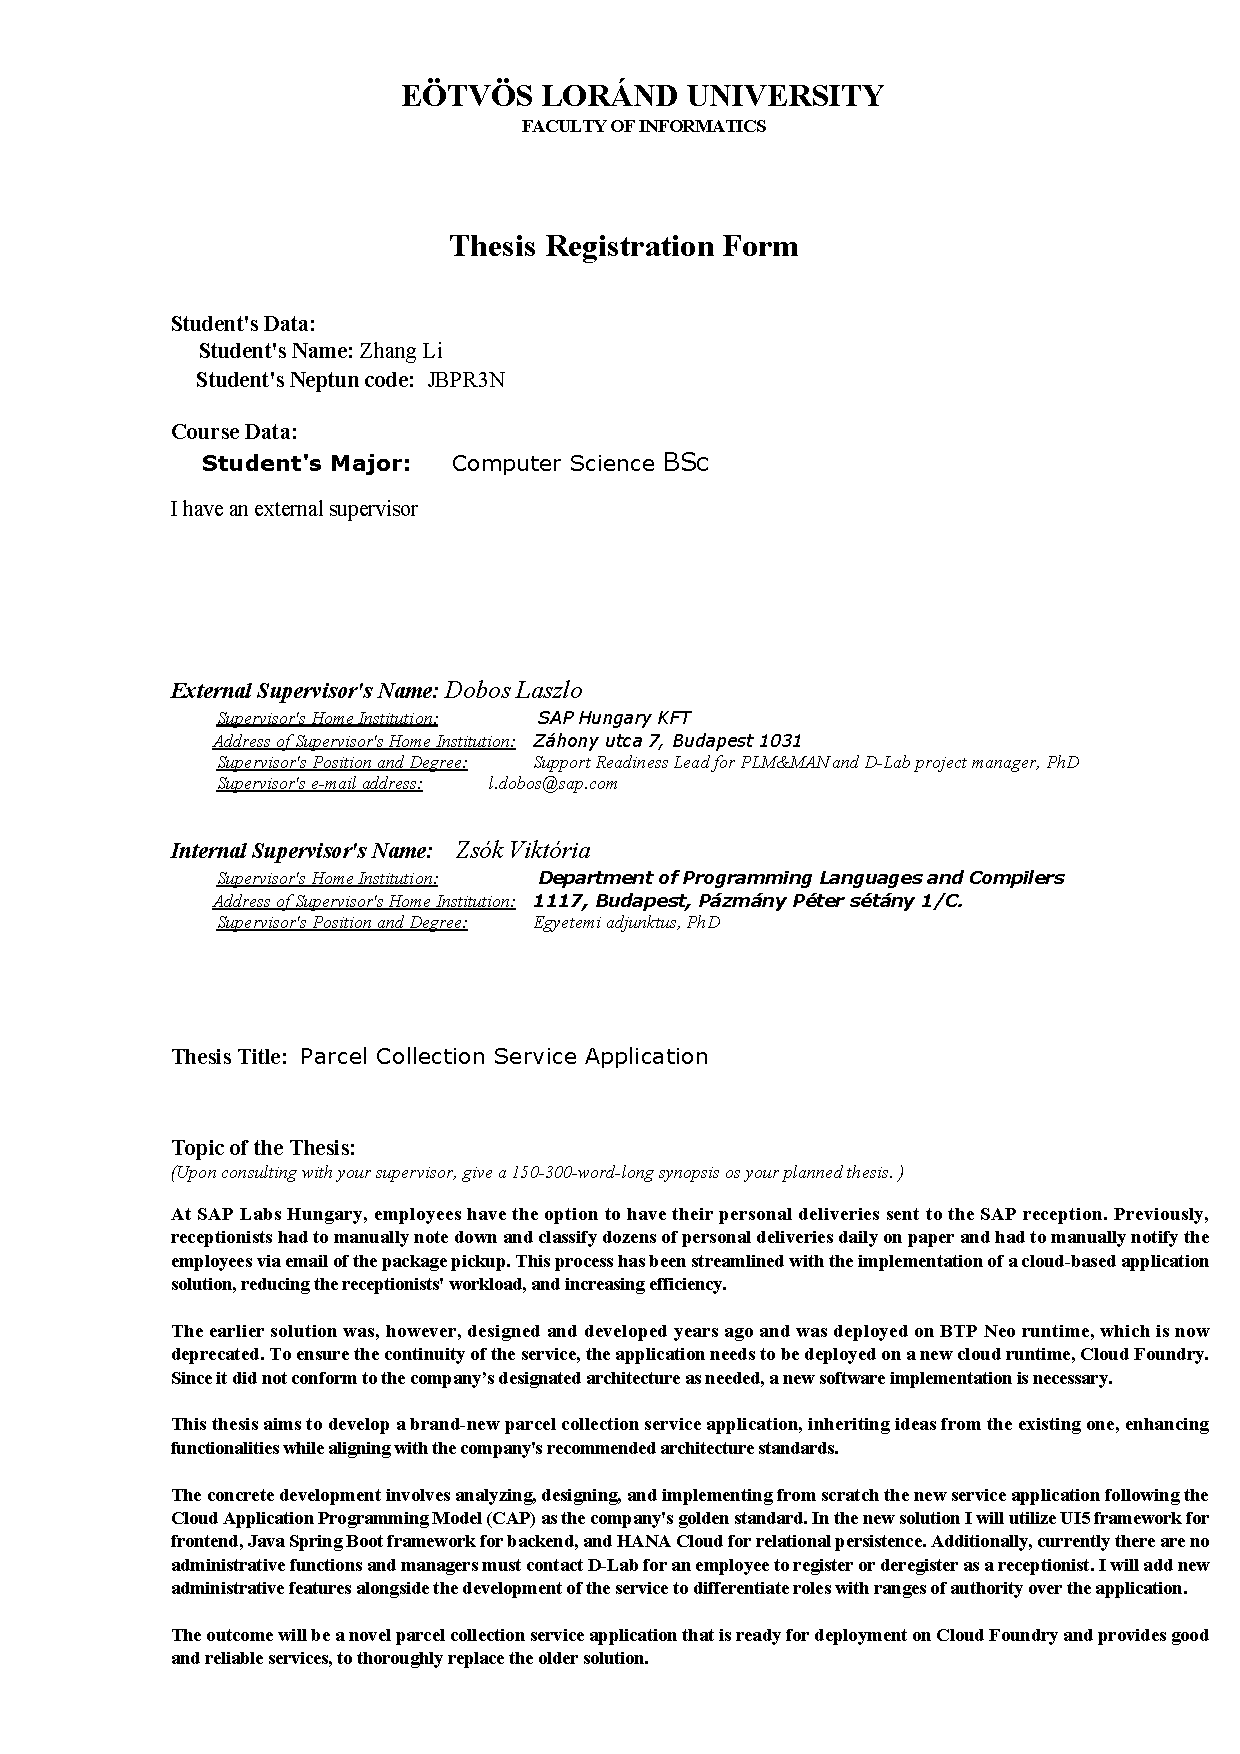
\includepdf{topicdeclaration.pdf}

% Table of contents (mandatory)
\tableofcontents
\cleardoublepage

% Main content
\chapter{Introduction}
\label{ch:intro}

\section{Motivation}
Alongside the rapid growth of e-commerce and delivery capability, waiting for delivery has became an unavoidable situation for a person. In most of the cases, parcels arrive during the working hours, and it is ineffective and not always possible for someone to stay for the delivery. Therefore, SAP \cite{sap} offers its employees with a solution, parcel collection service. Employees could deliver their personal deliveries to the address of the company. By the time it arrives, it is first accepted by the 24/7 reception desk and is able to be picked by the employee any time later.

Digital Lab is a team aiming to provide internal applications to improve employees' life at SAP. Throughout the years, dozens of solutions were created and deployed to SAP BTP \cite{btp} Neo platform \cite{neo}. With the deprecation of Neo, the old solutions will soon be forced to retire due to their dependence on the platform, including the parcel collection service.

This thesis creates a brand-new parcel collection application to fit in the gap. The application is designed to be platform independent and to optimize the using experience of every targeted groups of users (administrator, manager, receptionist and end-user). It provides a simplified work stream that is, receptionist register a new package, receptionist confirms a new package by allocating it a slot, employee confirms the pick up. It also provides the authorized party capabilities of managing the storage, parcels and delivery companies. Own histories can be reviewed by registered users.

The resulting solution consists of 6 interdependent applications consuming different services sharing the same database. The related information regarding the solution are collected in this thesis. The coming \autoref{sec:IntroSum} gives a quick preview of the upcoming chapters.

% Technically, the application is implemented as a MTA following CAP programming model and runs on SAP BTP, Cloud Foundry environment. It consists of 7 micro services. The data model and UI of the application is modeled and annotated with CDS language, which is the backbone of CAP. The back-end services are also defined in CDS and custom logic are implemented with the help of Java Spring Boot framework. 

\section{Summary}
\label{sec:IntroSum}

In the forthcoming chapters, a detailed exploration of the parcel collection application is compiled and presented. 

The \autoref{ch:user} contains the user documentation, in which the purpose and usage of application is explained. The chapter falls into three parts. In the first part, the basic business context is explained. Then in the second part, general prerequisites and related role concepts of the application are explained. After this, the third part focuses on the practical aspects tailored for end-users, receptionists, facility managers, and administrators. Role by role, the usages of each application are explained step by step, page after page embedded with rich images illustrations, providing any potential users with a clear idea of the goal of the application and the things can be done with. 

After this comes \autoref{ch:impl}, the developer documentation. This chapter reveals all critical technical details lies under the application. It illustrates the general application structure and logs the required local environments for potential future developments. It explains in details the architectures and implementations of front-end, back-end and data model. It also examines the testing ideas and procedures. 

Finally a conclusion (\autoref{ch:sum}) is attached, re-summarizing the solution and listing out the main take ways from the solution. It also concludes the potential improvements from a developer's perpect of view.

As readers progressing through the subsequent chapters, one will gradually get to know the application inside-out, from both user and developer perspectives. One can not only learn how to make use of the solution, but also how to further develop the application.
Here jumps to the user documentation (\autoref{ch:user}).


 % velit \cite{dahl1972structured}. euismod.\footnote{Maecenas a urna viverra, scelerisque nibh ut, malesuada ex.}

 % mus \cite{cormen2009algorithms,krasner1988mvc}. bibendum  \citeauthor{dijkstra1979goto}  purus \cite{dijkstra1979goto}. 

\cleardoublepage

\chapter{User documentation}
\label{ch:user}

This chapter is dedicated for the potential users. In \autoref{sec:GeneralRequisite}, the requisite of opening and using the application is listed. It also gives an introduction to the types of user roles within the solution, to enable the users to navigating through the thesis and find their related information quickly.

Then in the following sections (\autoref{sec:UdocEndUser}, \autoref{sec:UdocReceptionist}, \autoref{sec:UdocFacilityManager}, \autoref{sec:UdocAdministrator}), which are titled by the roles, collects the use guide of each accessible applications.

\section{General Requisite}
\label{sec:GeneralRequisite}

This solution is designed for the internal usage within SAP supporting the parcel collection service providing to the employees. The solution enables the complete digitalization and standardization of the parcel signing and management processes. The service provided by the solution can be summarised into three parts: the management of possible storage locations of the parcels (administration side), the management of possible companies of the parcels  (administration side) and the management of the packages (both receptionist side and user side).  The solution is realized through six applications as tiles on the Fiori launchpad \cite{flp}: \textbf{My packages}, \textbf{Pickup packages}, \textbf{Register Packages}, \textbf{Manage packages}, \textbf{Manage Companies} and \textbf{Manage Storages} partitioned into 3 sections: \textbf{My Home}, \textbf{Pacel Handling}, \textbf{Administration}, as shown in \autoref{fig:ApplicationLaunchScreen}.

\begin{figure}[H]
	\centering
	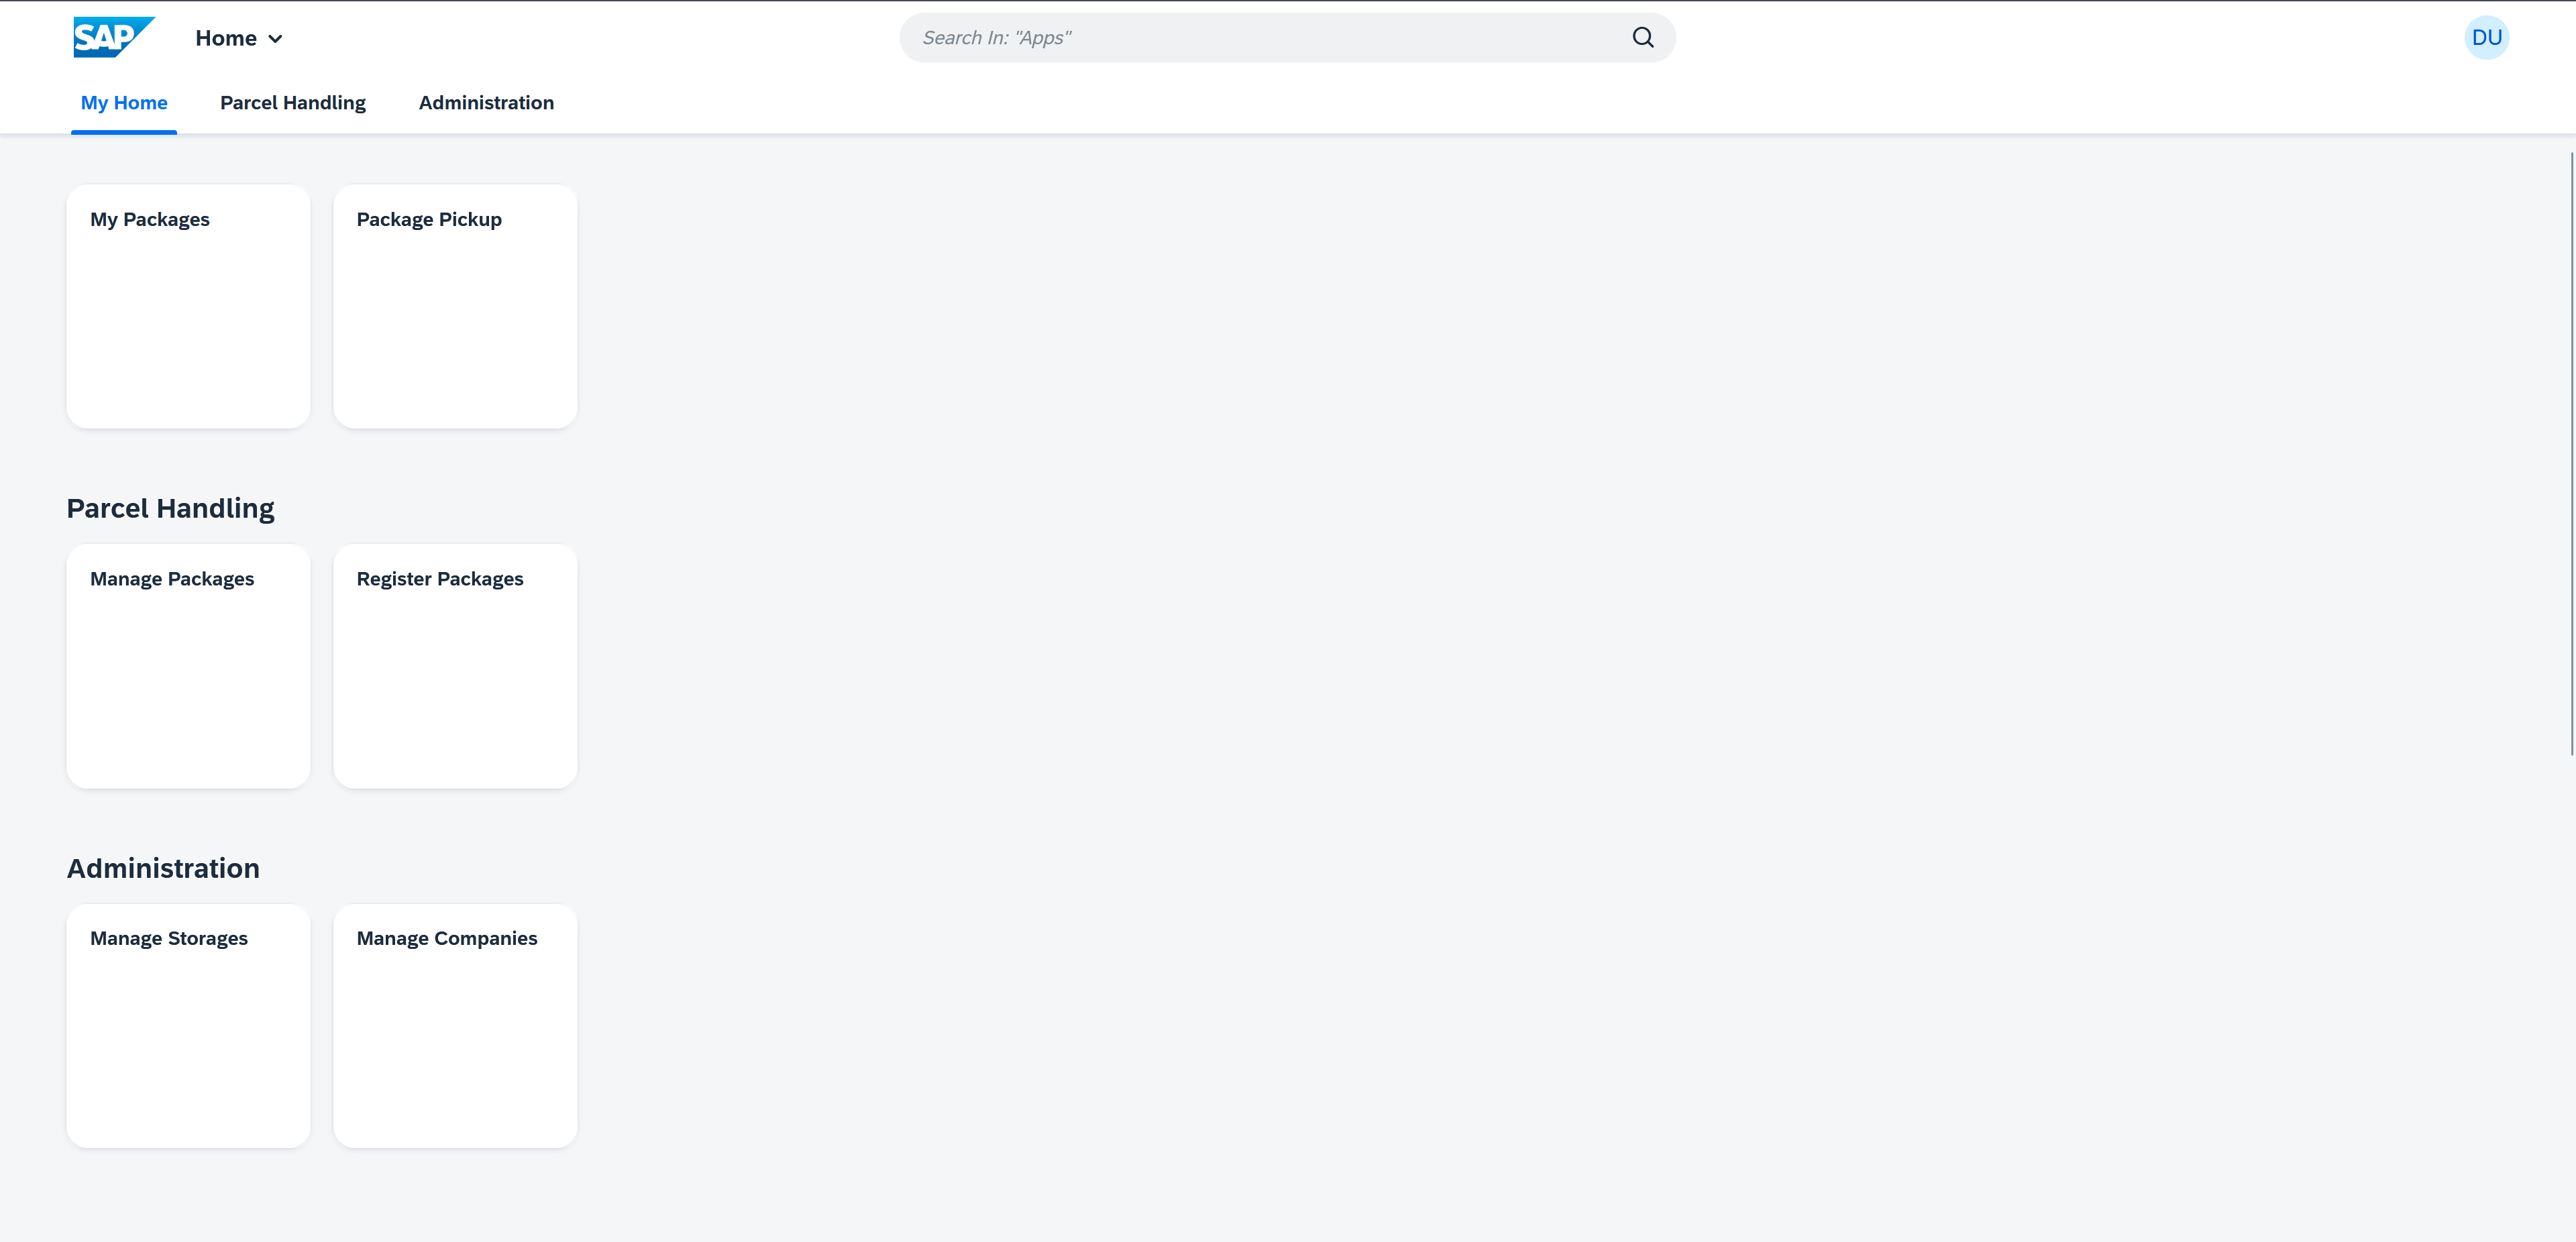
\includegraphics[width=1\linewidth]{images/user_doc/overviews/sandbox.png}
	\caption{Application Launch Screen}
	\label{fig:ApplicationLaunchScreen}
\end{figure}


In order to use any of the application, one has to hold an SAP registered device (computer/tablet/phone) and is able to use a supported browser with stable internet connection. In order to use \textbf{Pickup packages} application, one has to hold an SAP registered smart phone. 

In order to mock use the application in local environment, please move the the developer documentation (\autoref{ch:impl}) and follow the set up steps. 

Four different roles are specified for the application and an authenticated user is limited to applications dedicated to their assigned roles. In the coming sections the usage guides are documented sectioned by the roles. Hereby lists the meaning of each role under the thesis context and feel ease to jump to the related section by clicking section links.

\begin{description}
	\item[End User (\autoref{sec:UdocEndUser})] Any SAP employee who holds an SAP registered device and would like to use the parcel collection service.
	\item[Receptionist (\autoref{sec:UdocReceptionist})] Registered receptionist working at the reception and is responsible to serve the parcel collection service. Assigned "Receptionist" role on BTP.
	\item[Facility Manager (\autoref{sec:UdocFacilityManager})] Authorised user who is responsible for maintaining the delivery companies and storage slots information. Assigned "FacilityManager" role on BTP.
	\item[Administrator (\autoref{sec:UdocAdministrator})] The master user who can access to any of the applications. Assigned "Administrator" role on BTP.
\end{description}

In case one is accessing the applications through browser from BTP platform \cite{btp}, the login process is done automatically. Otherwise, if one is running the application locally, a browser pop up will appear (\autoref{fig:LocalLoginPopUp}) and mock user (See existing mock credentials in \autoref{sec:D-security}) should be entered.
In the case of any user trying to accessing an unauthorised application, connection will fail. (\autoref{fig:IllegalAccesstoUnauthorised Applications})

\begin{figure}[H]
	\centering
	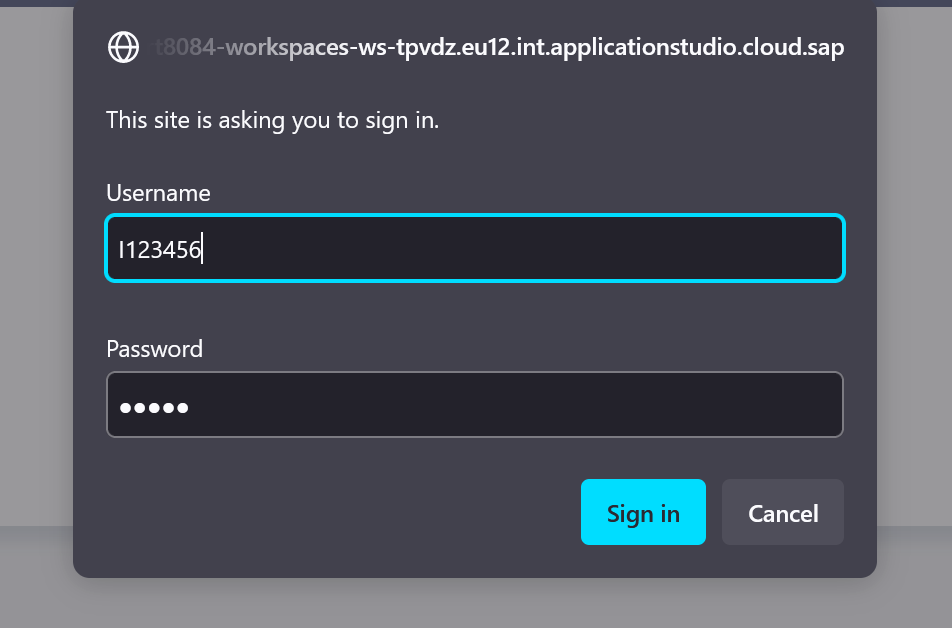
\includegraphics[width=0.5\linewidth]{images/user_doc/overviews/localLogin.png}
	\caption{Local Login Pop Up}
	\label{fig:LocalLoginPopUp}
\end{figure}

\begin{figure}[H]
	\centering
	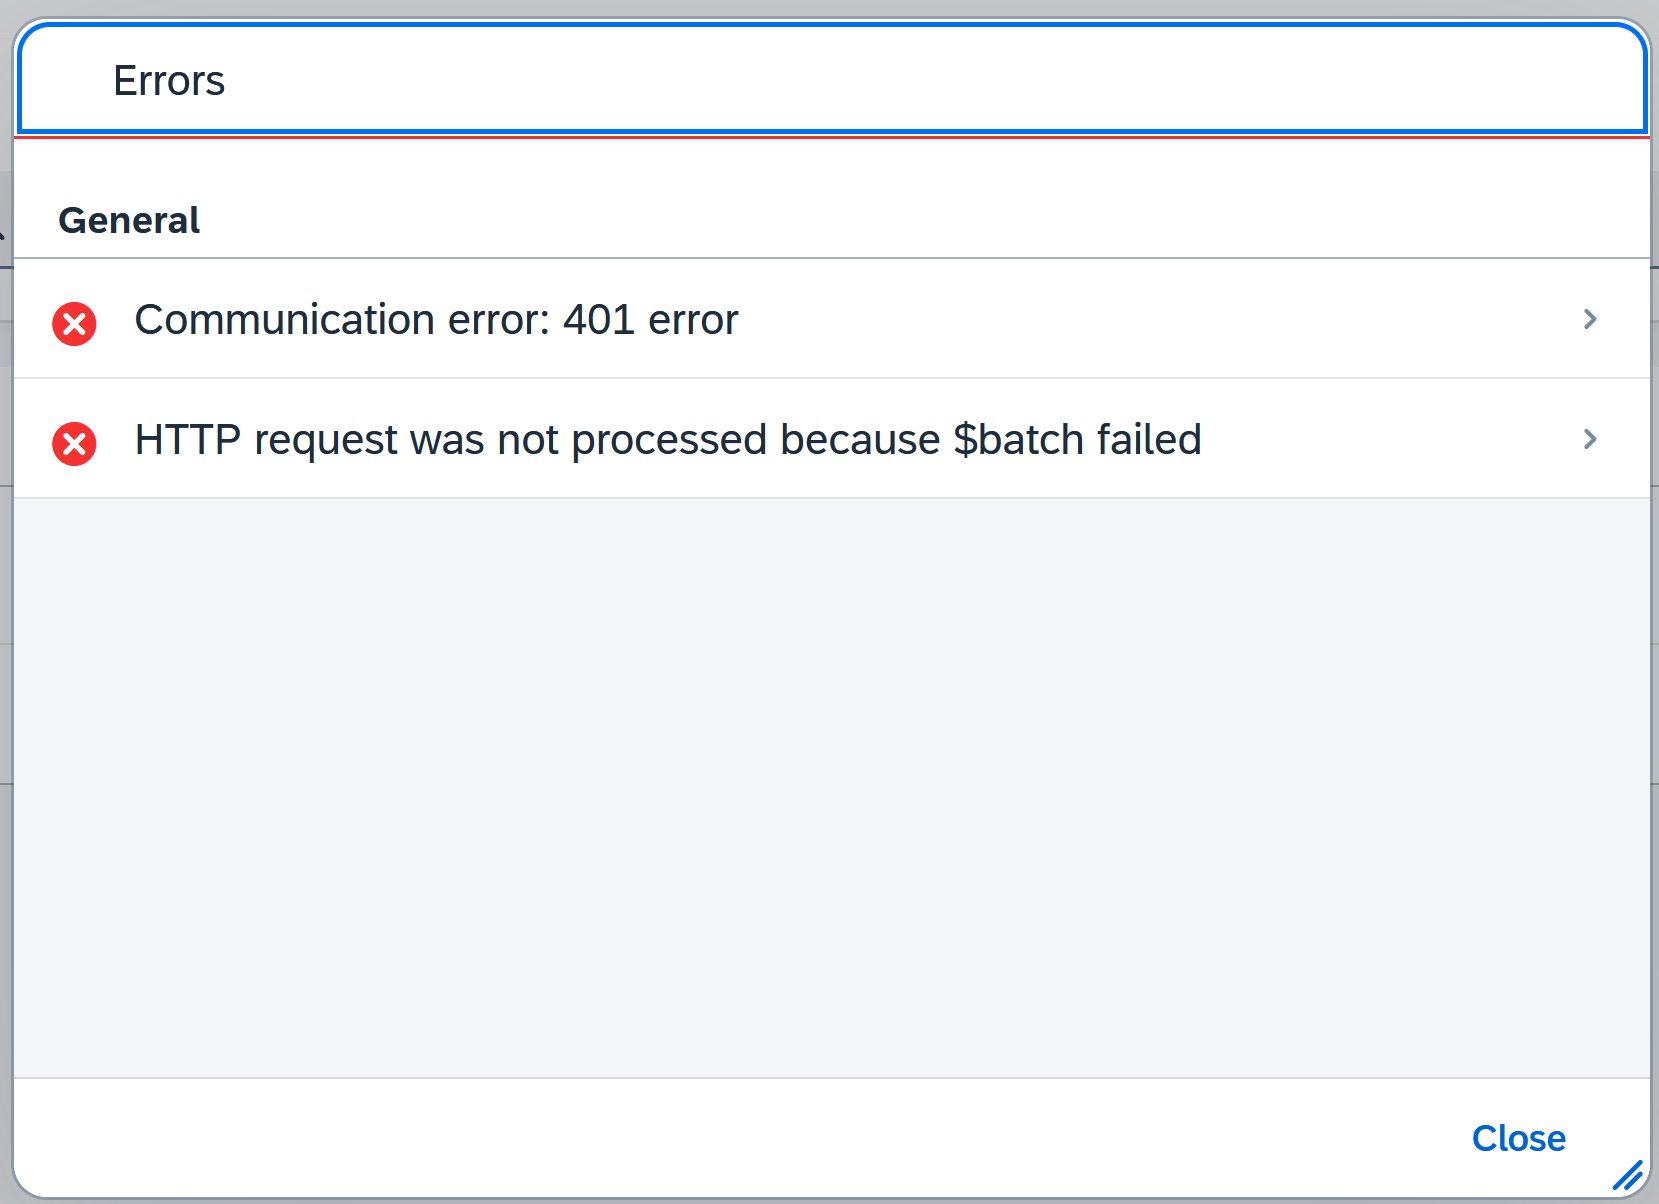
\includegraphics[width=0.5\linewidth]{images/user_doc/overviews/ConnectionError1.png}
	\caption{Illegal Access to Unauthorised Applications - Possible Error}
	\label{fig:IllegalAccesstoUnauthorised Applications}
\end{figure}

\pagebreak

\section{End User}
\label{sec:UdocEndUser}

As a logged in \textbf{End User}, one is granted to access the two applications under the \textbf{My Home} section, namely \textbf{My Packages} (\autoref{subsec:ph}) and \textbf{Package Pickup} (\autoref{subsec:pp}). \textbf{End User} can quick jump to the section by left clicking the "My Home" tab. \textbf{End User} can enter the application by left click the tiles. (\autoref{fig:EndUserApplications})

\begin{figure}[H]
	\centering
	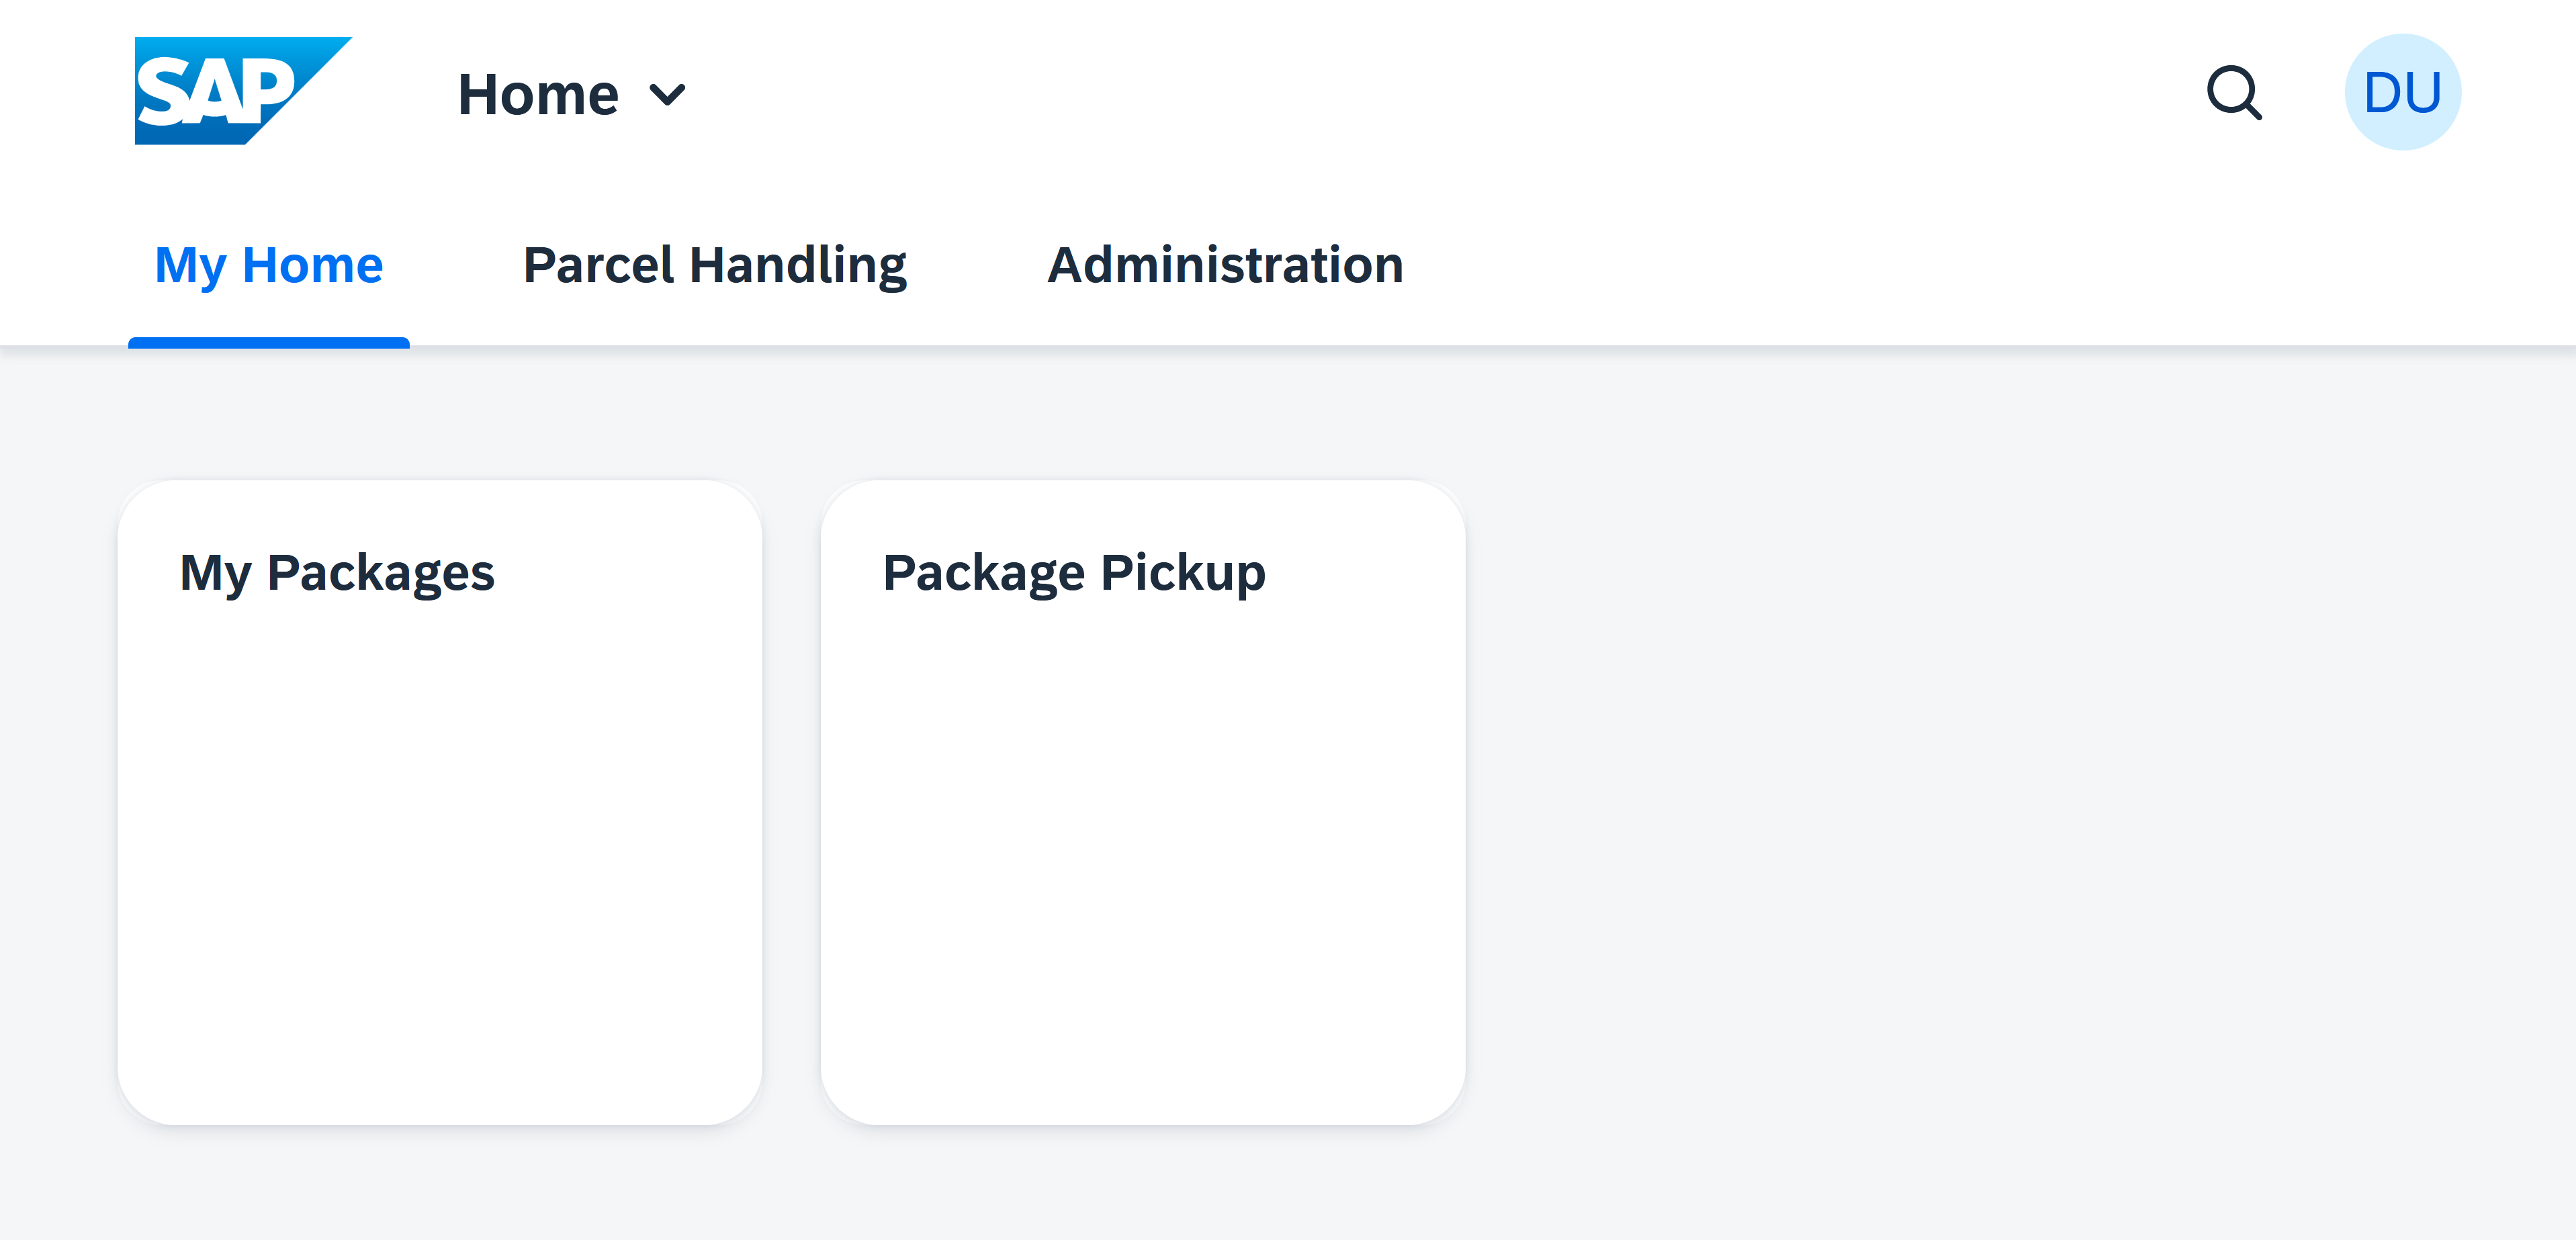
\includegraphics[width=1\linewidth]{images/user_doc/overviews/MyHomeTab.png}
	\caption{End User Applications}
	\label{fig:EndUserApplications}
\end{figure}


% ----------------------- MY PACKAGES ----------------------------
% 
%  ---------------------------------------------------------------

\subsection{My Packages}
\label{subsec:ph}

The \textbf{My Packages} application is here for any \textbf{End User} (See \autoref{sec:UdocEndUser} for all related applications) who would want to check his/her own packages. One can only see one's own packages. 
The summarized main actions the \textbf{End User} can take within the application are listed here:

\begin{compactenum}
	\item Browse the owned package history.
        \begin{compactenum}
        	\item Filter possibility.
            \item List report for packages.
        \end{compactenum}
\end{compactenum}

\subsubsection{Home Screen - Overview}
As an \textbf{End User}, after clicking at the application tile, is redirected to the "Home Screen" (\autoref{fig:HistoryHome}), which is the main and only screen of this application. The upper part displays the search bar and the possible filters. While the lower part displays the list of packages. The information provides for each packages are: \textbf{Type} (the type of the package, existing types are newspaper, letter and normal), \textbf{Status} (the status of the package, existing status are new, confirmed and picked up), \textbf{Delivery Company} (the delivery company of the package), \textbf{Delivery Time} (the confirmation time of the package, if applicable), \textbf{Pickup Time} (the picked up time of the package, if applicable).

\begin{figure}[H]
	\centering
	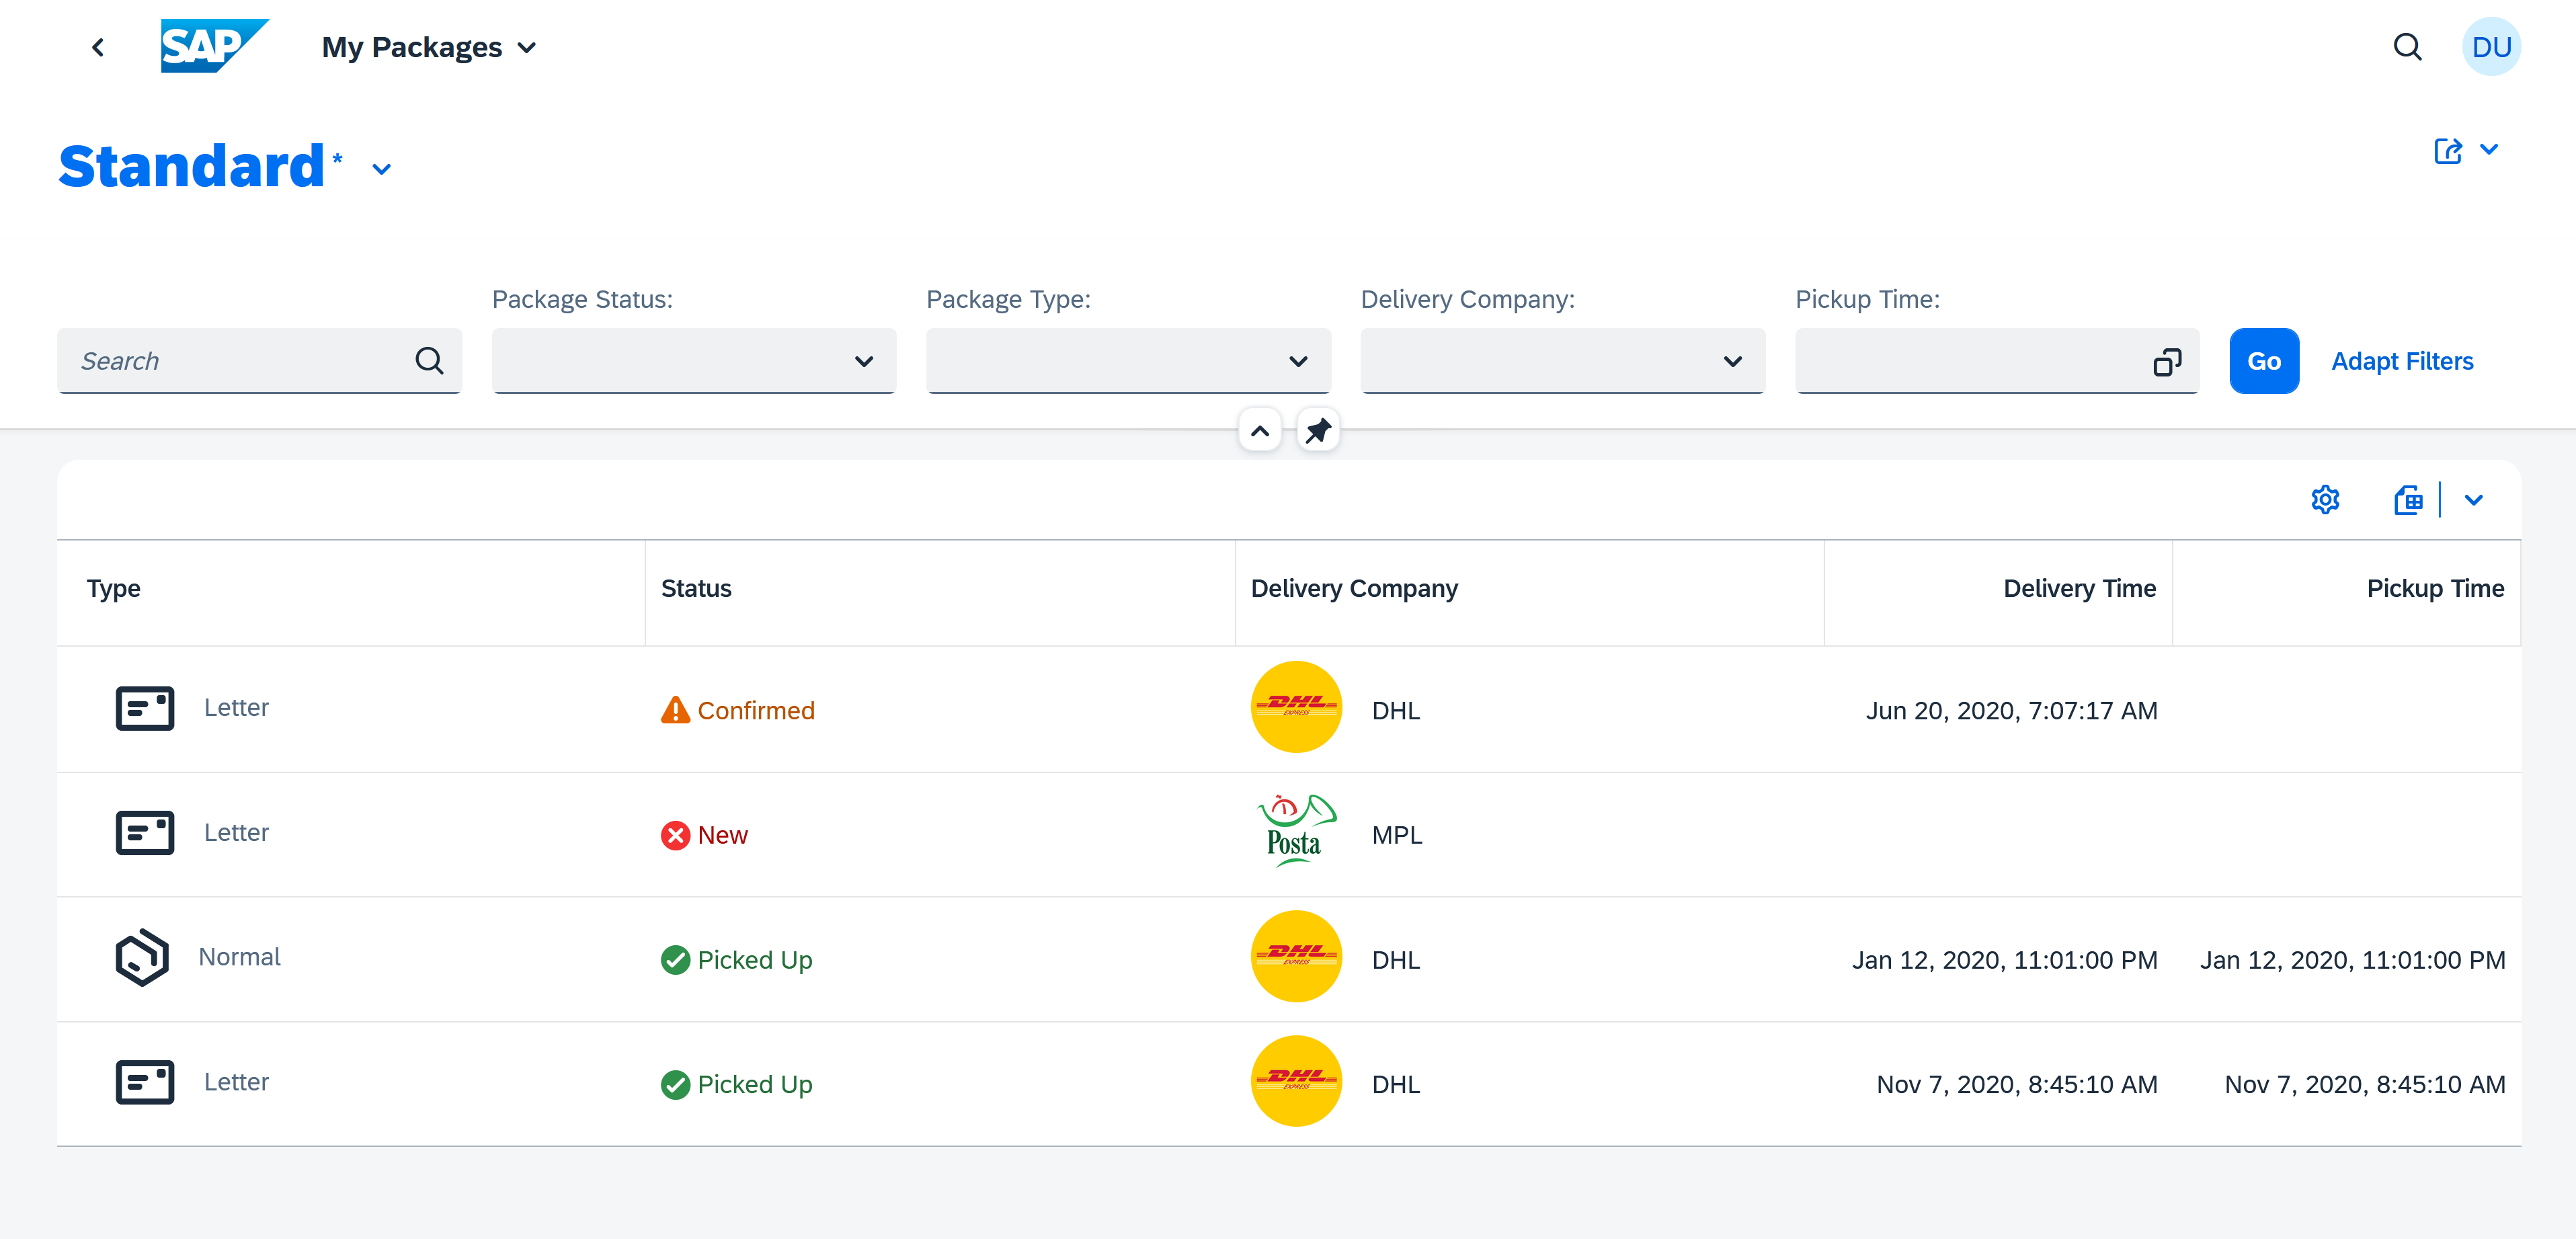
\includegraphics[width=1\linewidth]{images/user_doc/myPack/overview.png}
	\caption{History Home Screen - Overview}
	\label{fig:HistoryHome}
\end{figure}

\subsubsection{Home Screen - Filter Usage}
One can type in free text of any possible content of the column in the "Search Bar" (\autoref{fig:mpSearchBar}). The free text supports in-completed keywords and is case insensitive. 
One can use the default filters (\textbf{Status} (drop down), \textbf{Type} (drop down), \textbf{Delivery Company} (drop down) and \textbf{Pickup Time} (time entry) (\autoref{fig:MPDF}). For drop down filters, one can click at the small drop down arrow and select zero to many options. For time entry, one shall click at the "double box" (filter help) on the right of the filter box. This will pops up a dialog, at where one can select the desired filtering option and enter the time with the clock uitility (\autoref{fig:PHAjustTimeFilters}). One can also access to more filters (\textbf{Delivery Time} (time entry) by clicking at "Adapt Filters". (\autoref{fig:mpMOreFilterAdaption}) While adjusting the filtering values, the list view is temporarily locked. After adjusting the filtering values, run the filter by clicking the "Go" Button. (\autoref{fig:PHAjustFilters-2})

\begin{figure}[H]
	\centering
	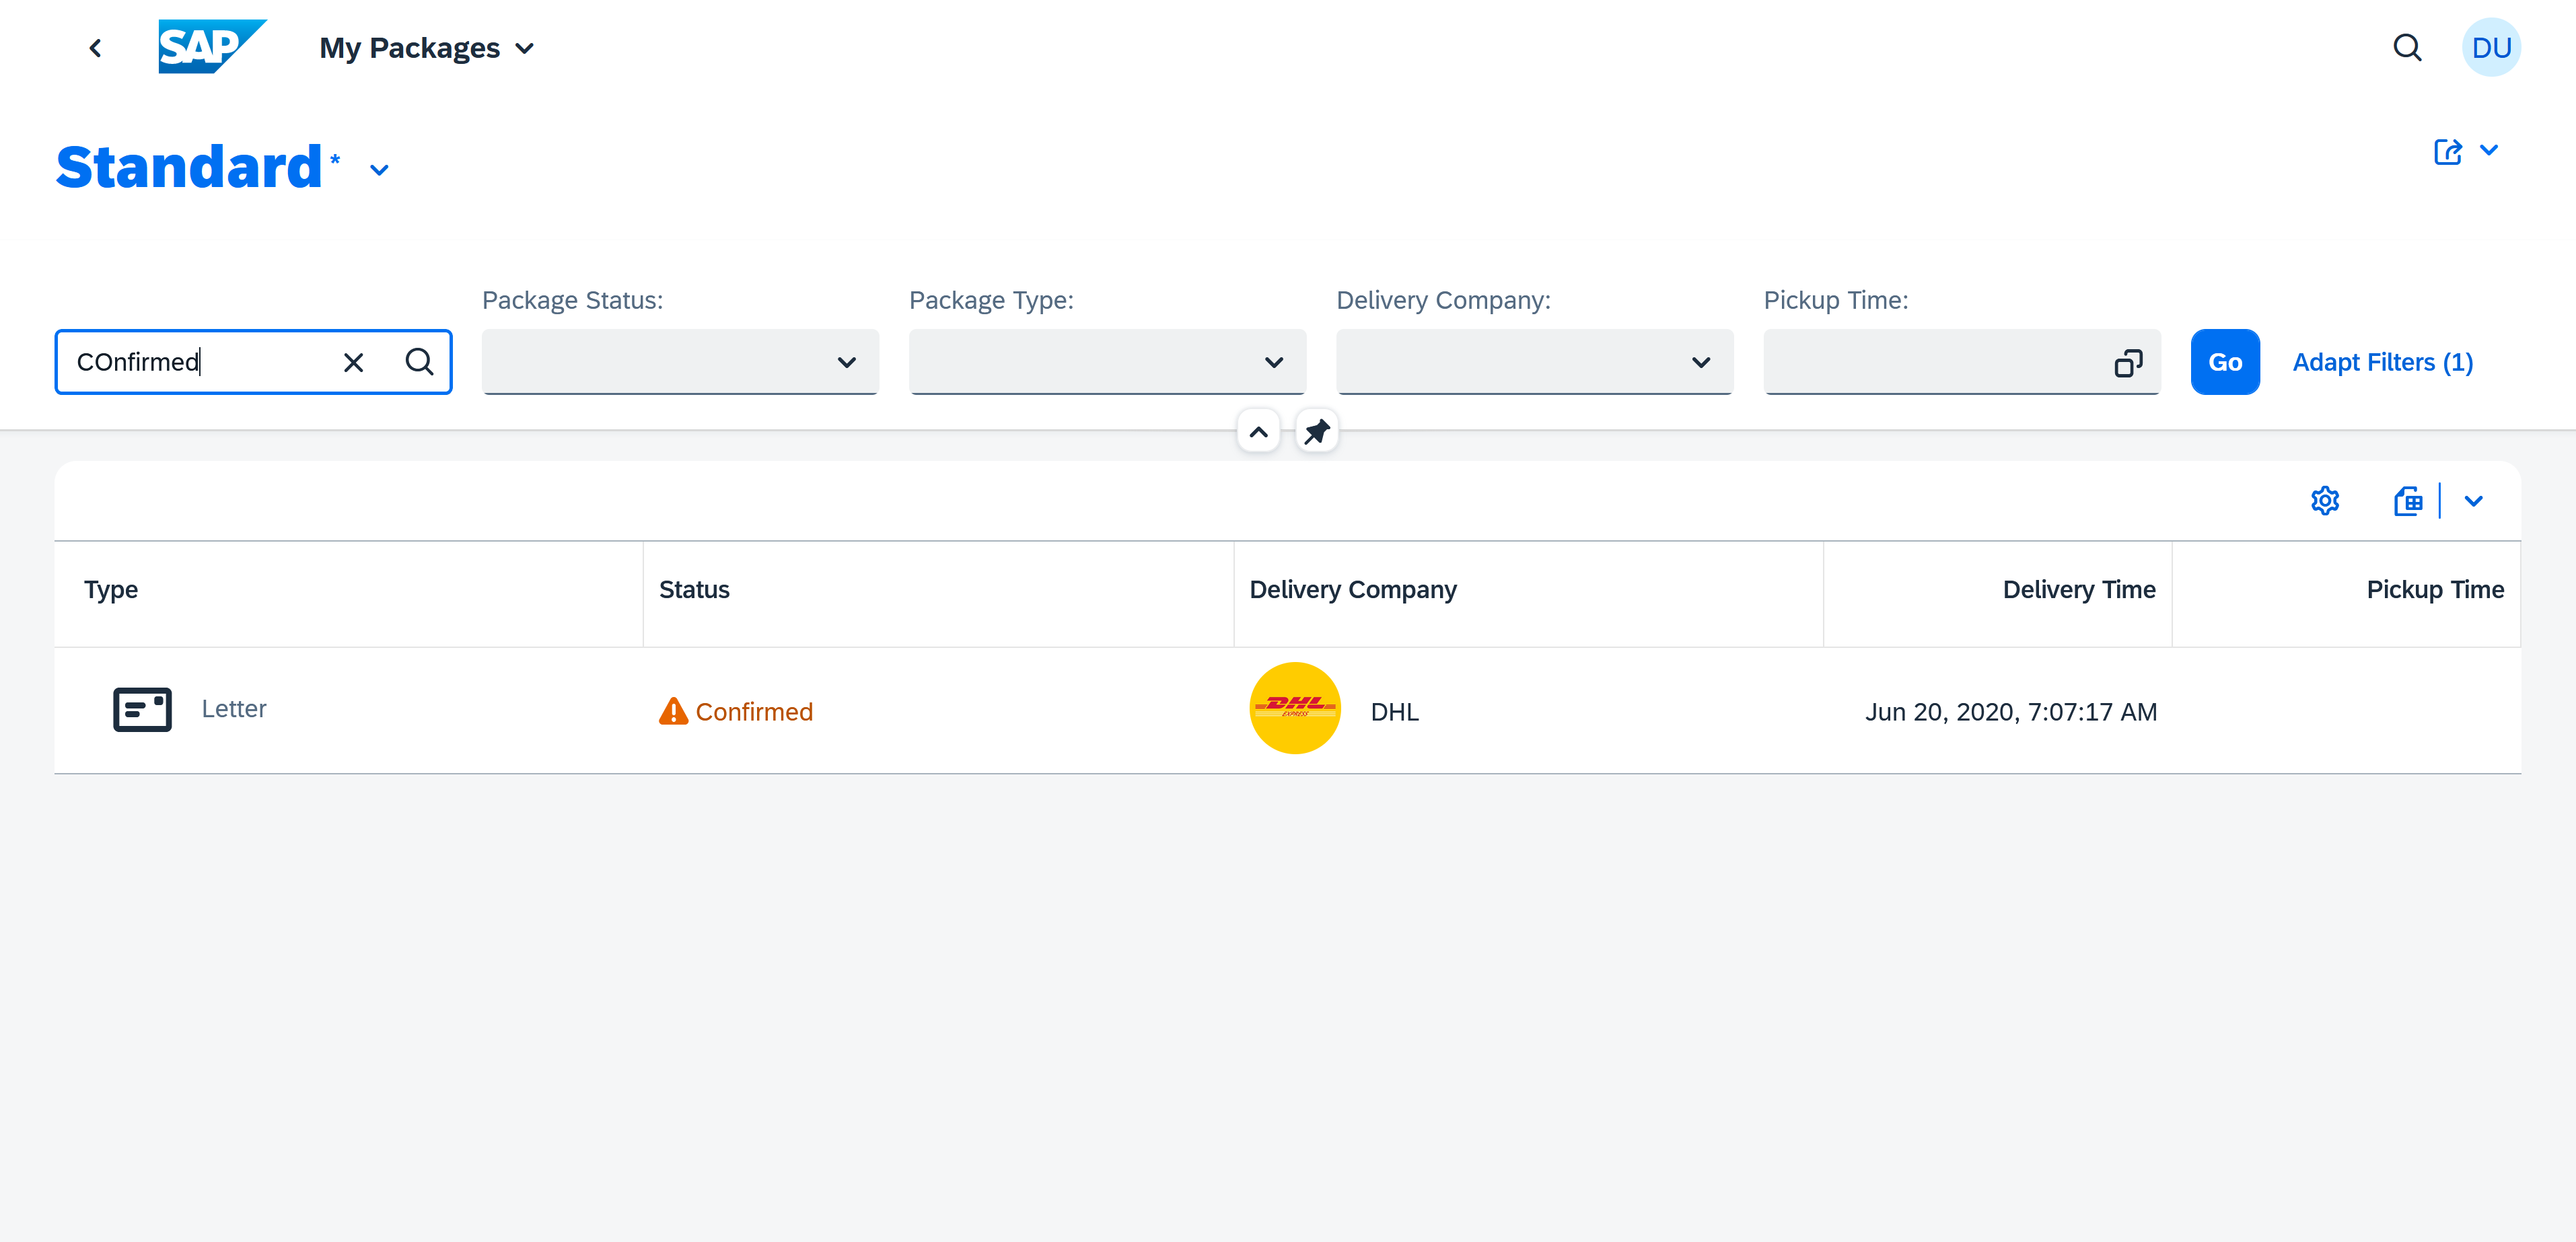
\includegraphics[width=1\linewidth]{images/user_doc/myPack/searchbar.png}
	\caption{My Package Home Screen - Search Bar}
	\label{fig:mpSearchBar}
\end{figure}


\begin{figure}[H]
	\centering
	\subcaptionbox{Status Filter}{
		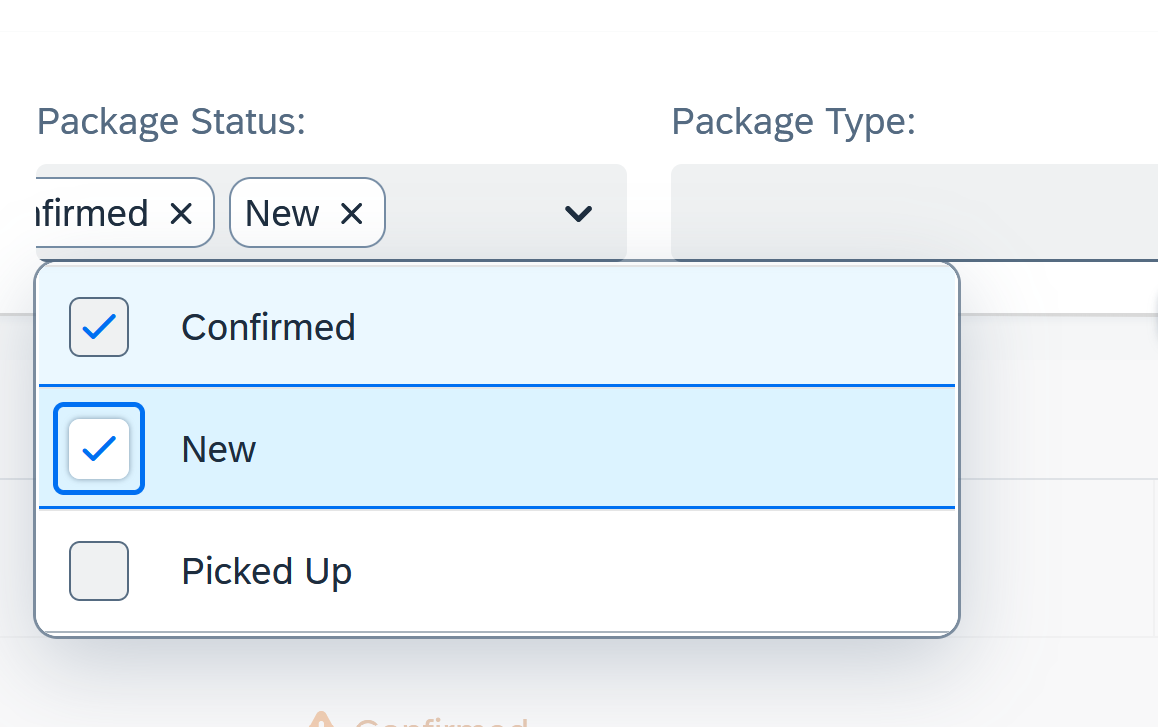
\includegraphics[width=0.45\linewidth]{images/user_doc/myPack/statusFIlter.png}}
	\hspace{5pt}
	\subcaptionbox{Type Filter}{
		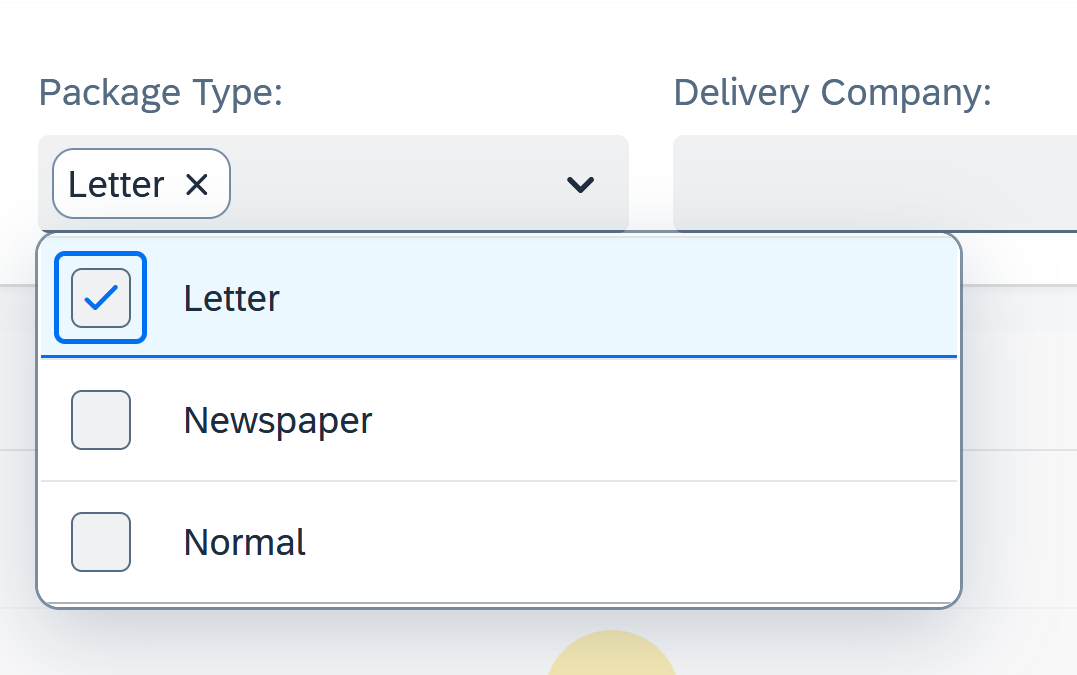
\includegraphics[width=0.45\linewidth]{images/user_doc/myPack/typeFIlter.png}}

    \subcaptionbox{Company Filter}{
		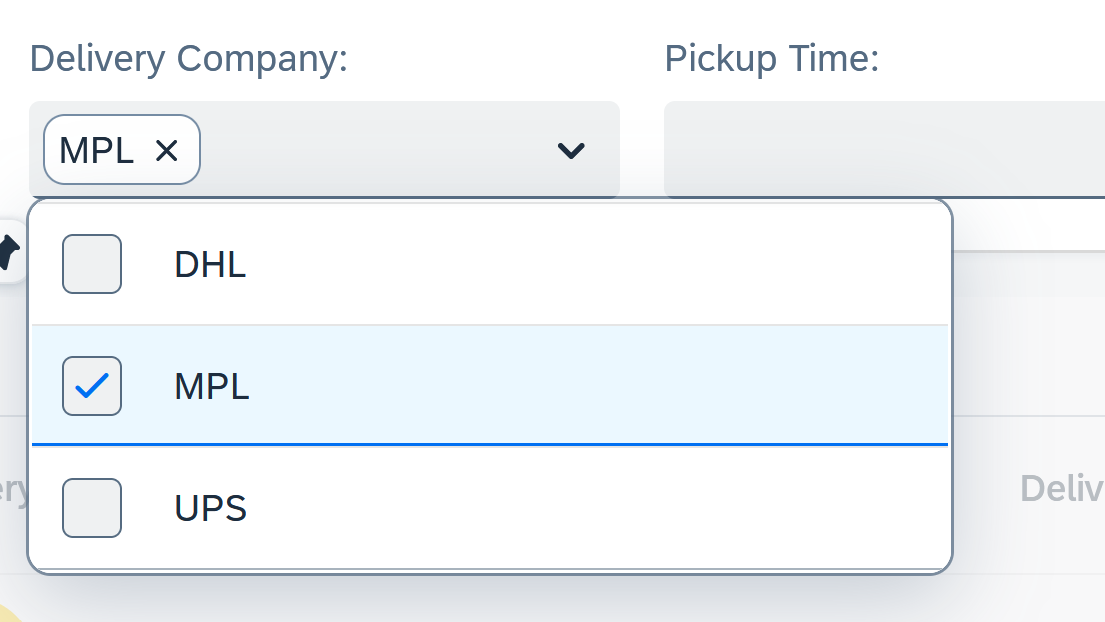
\includegraphics[width=0.45\linewidth]{images/user_doc/myPack/companyFilter.png}}
	\hspace{5pt}
	\subcaptionbox{Time Filter}{
		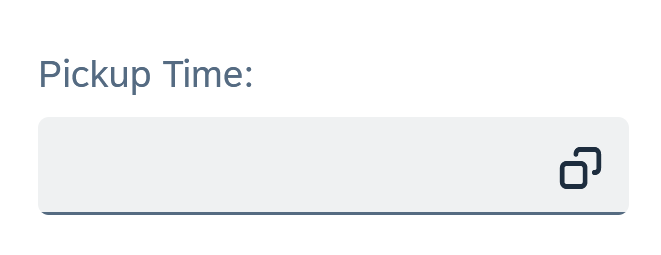
\includegraphics[width=0.45\linewidth]{images/user_doc/myPack/timeFilter.png}}
	\caption{My Package Home Screen - Default Filters}
	\label{fig:MPDF}
\end{figure}

\begin{figure}[H]
		\centering
	\subcaptionbox{Time Filter Options Selections}{
		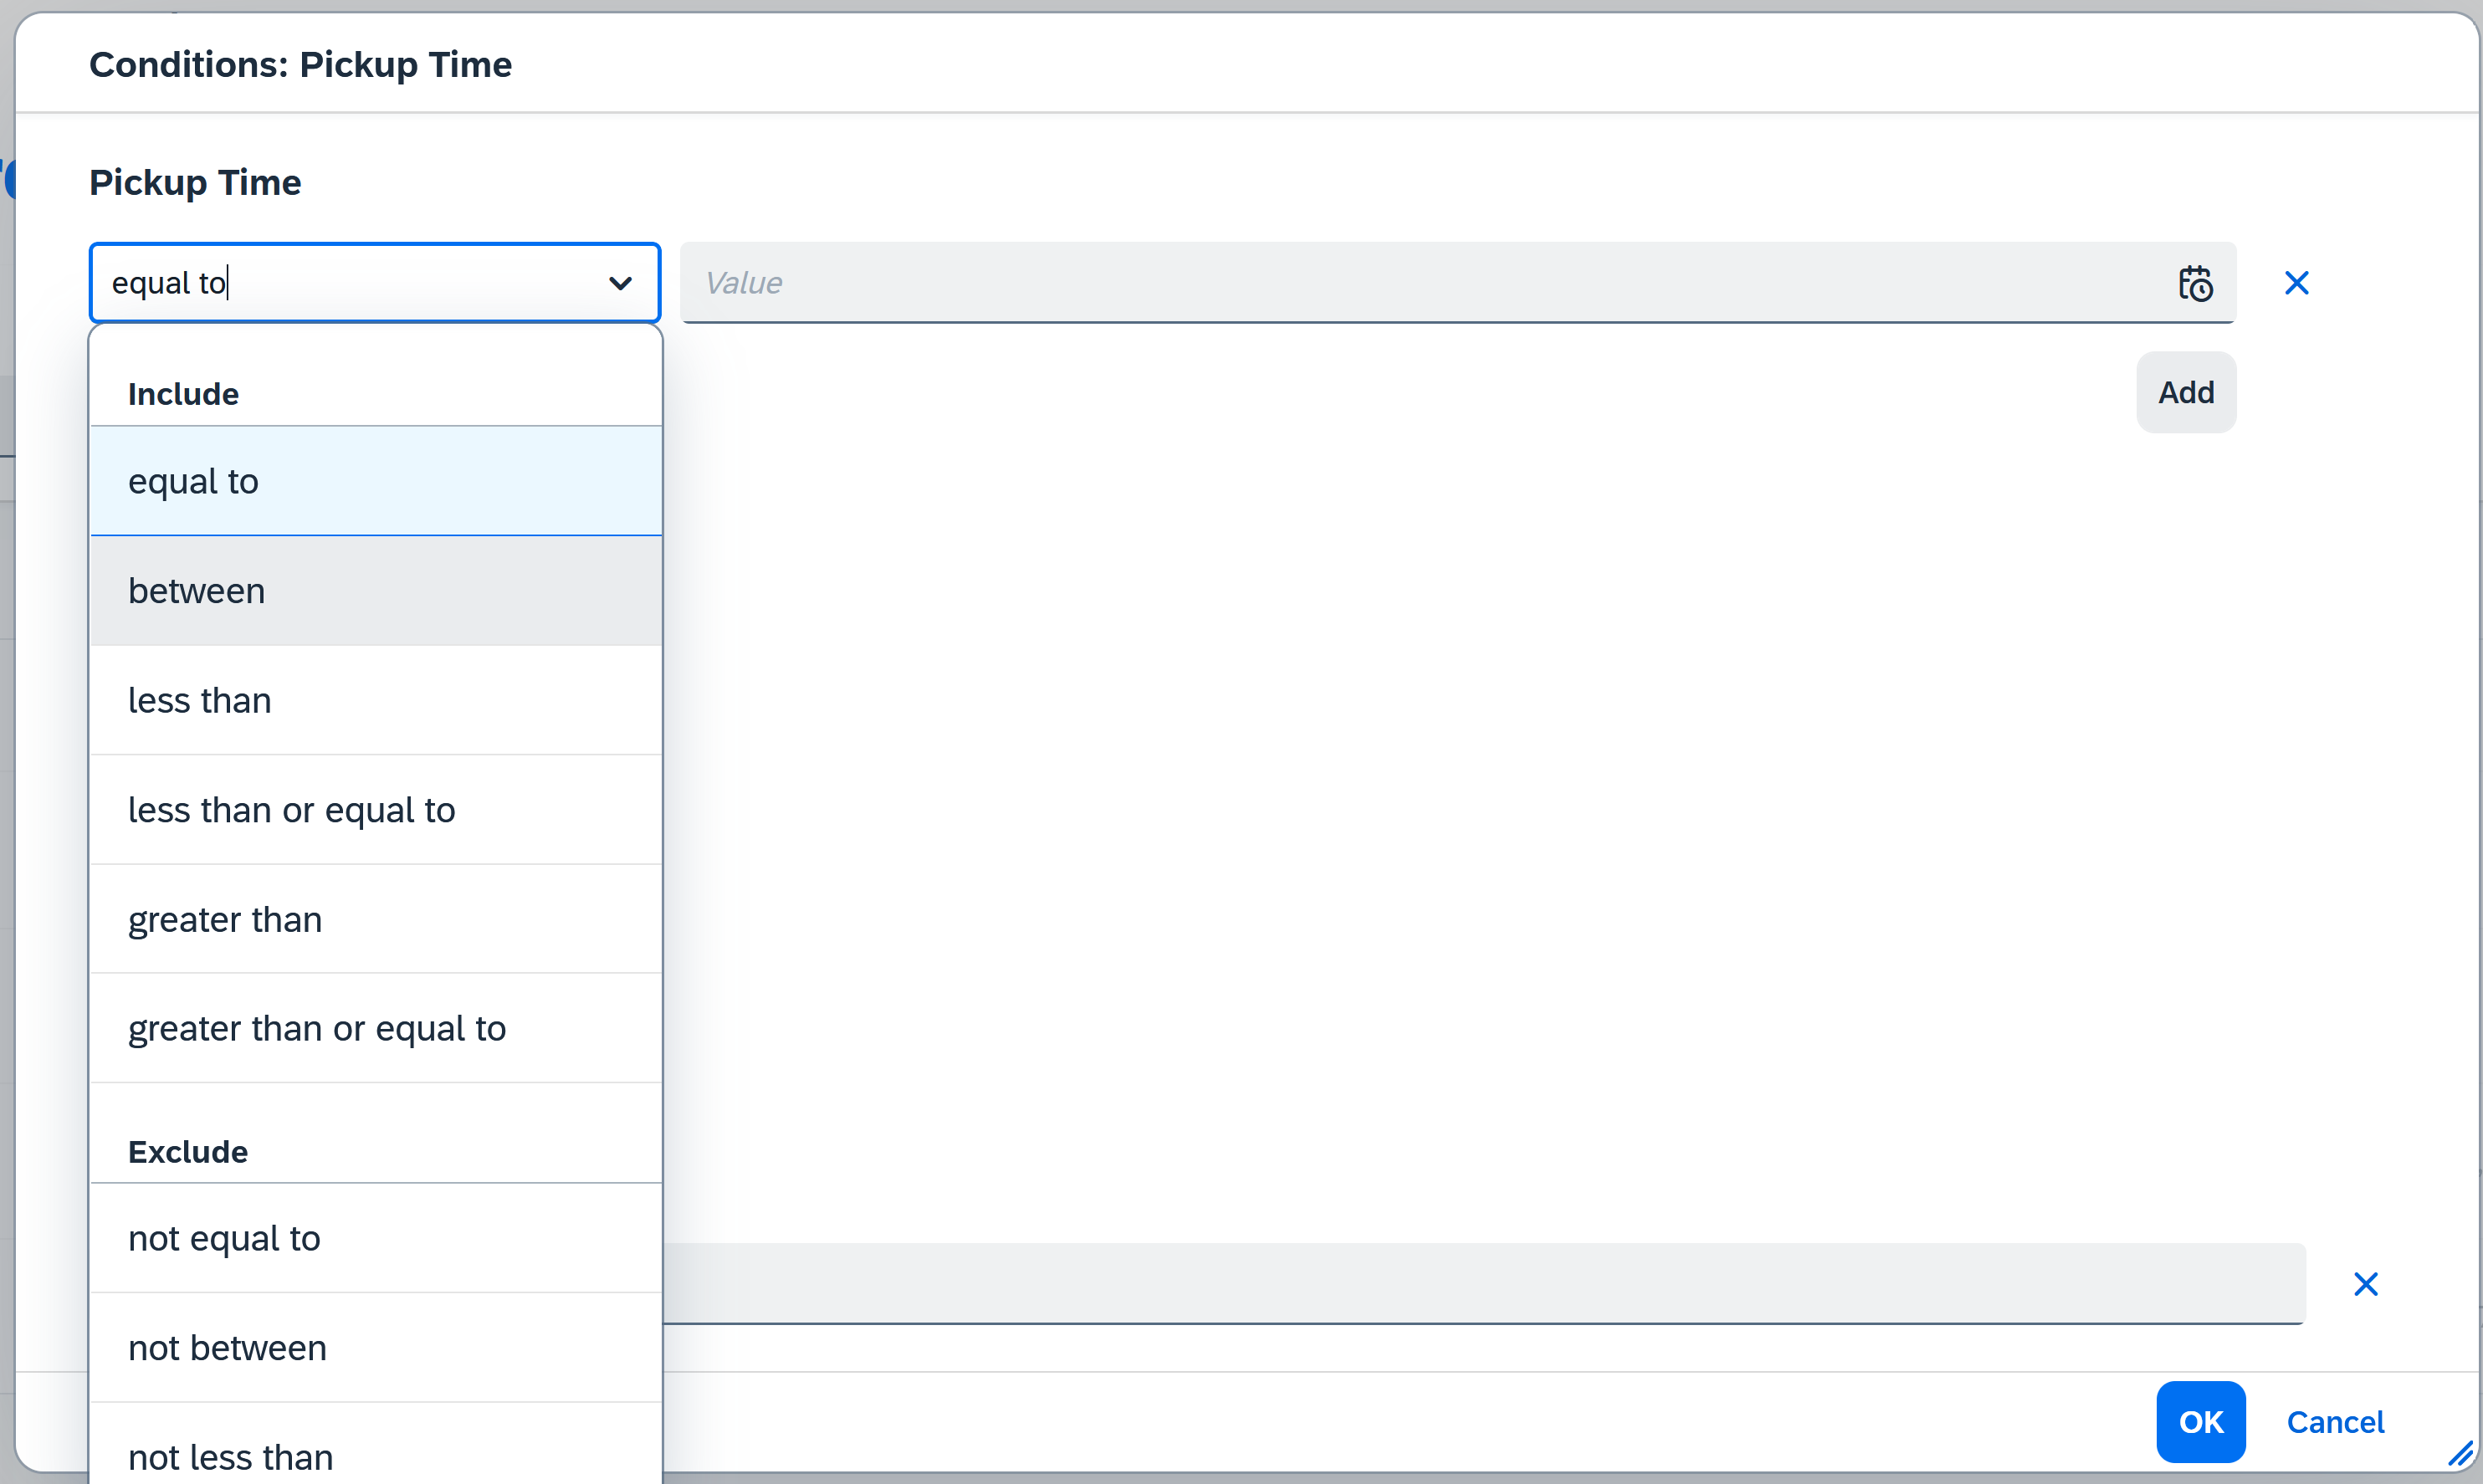
\includegraphics[width=0.45\linewidth]{images/user_doc/myPack/timeFilter_Usage1.png}}
	\hspace{5pt}
	\subcaptionbox{Time Entry}{
		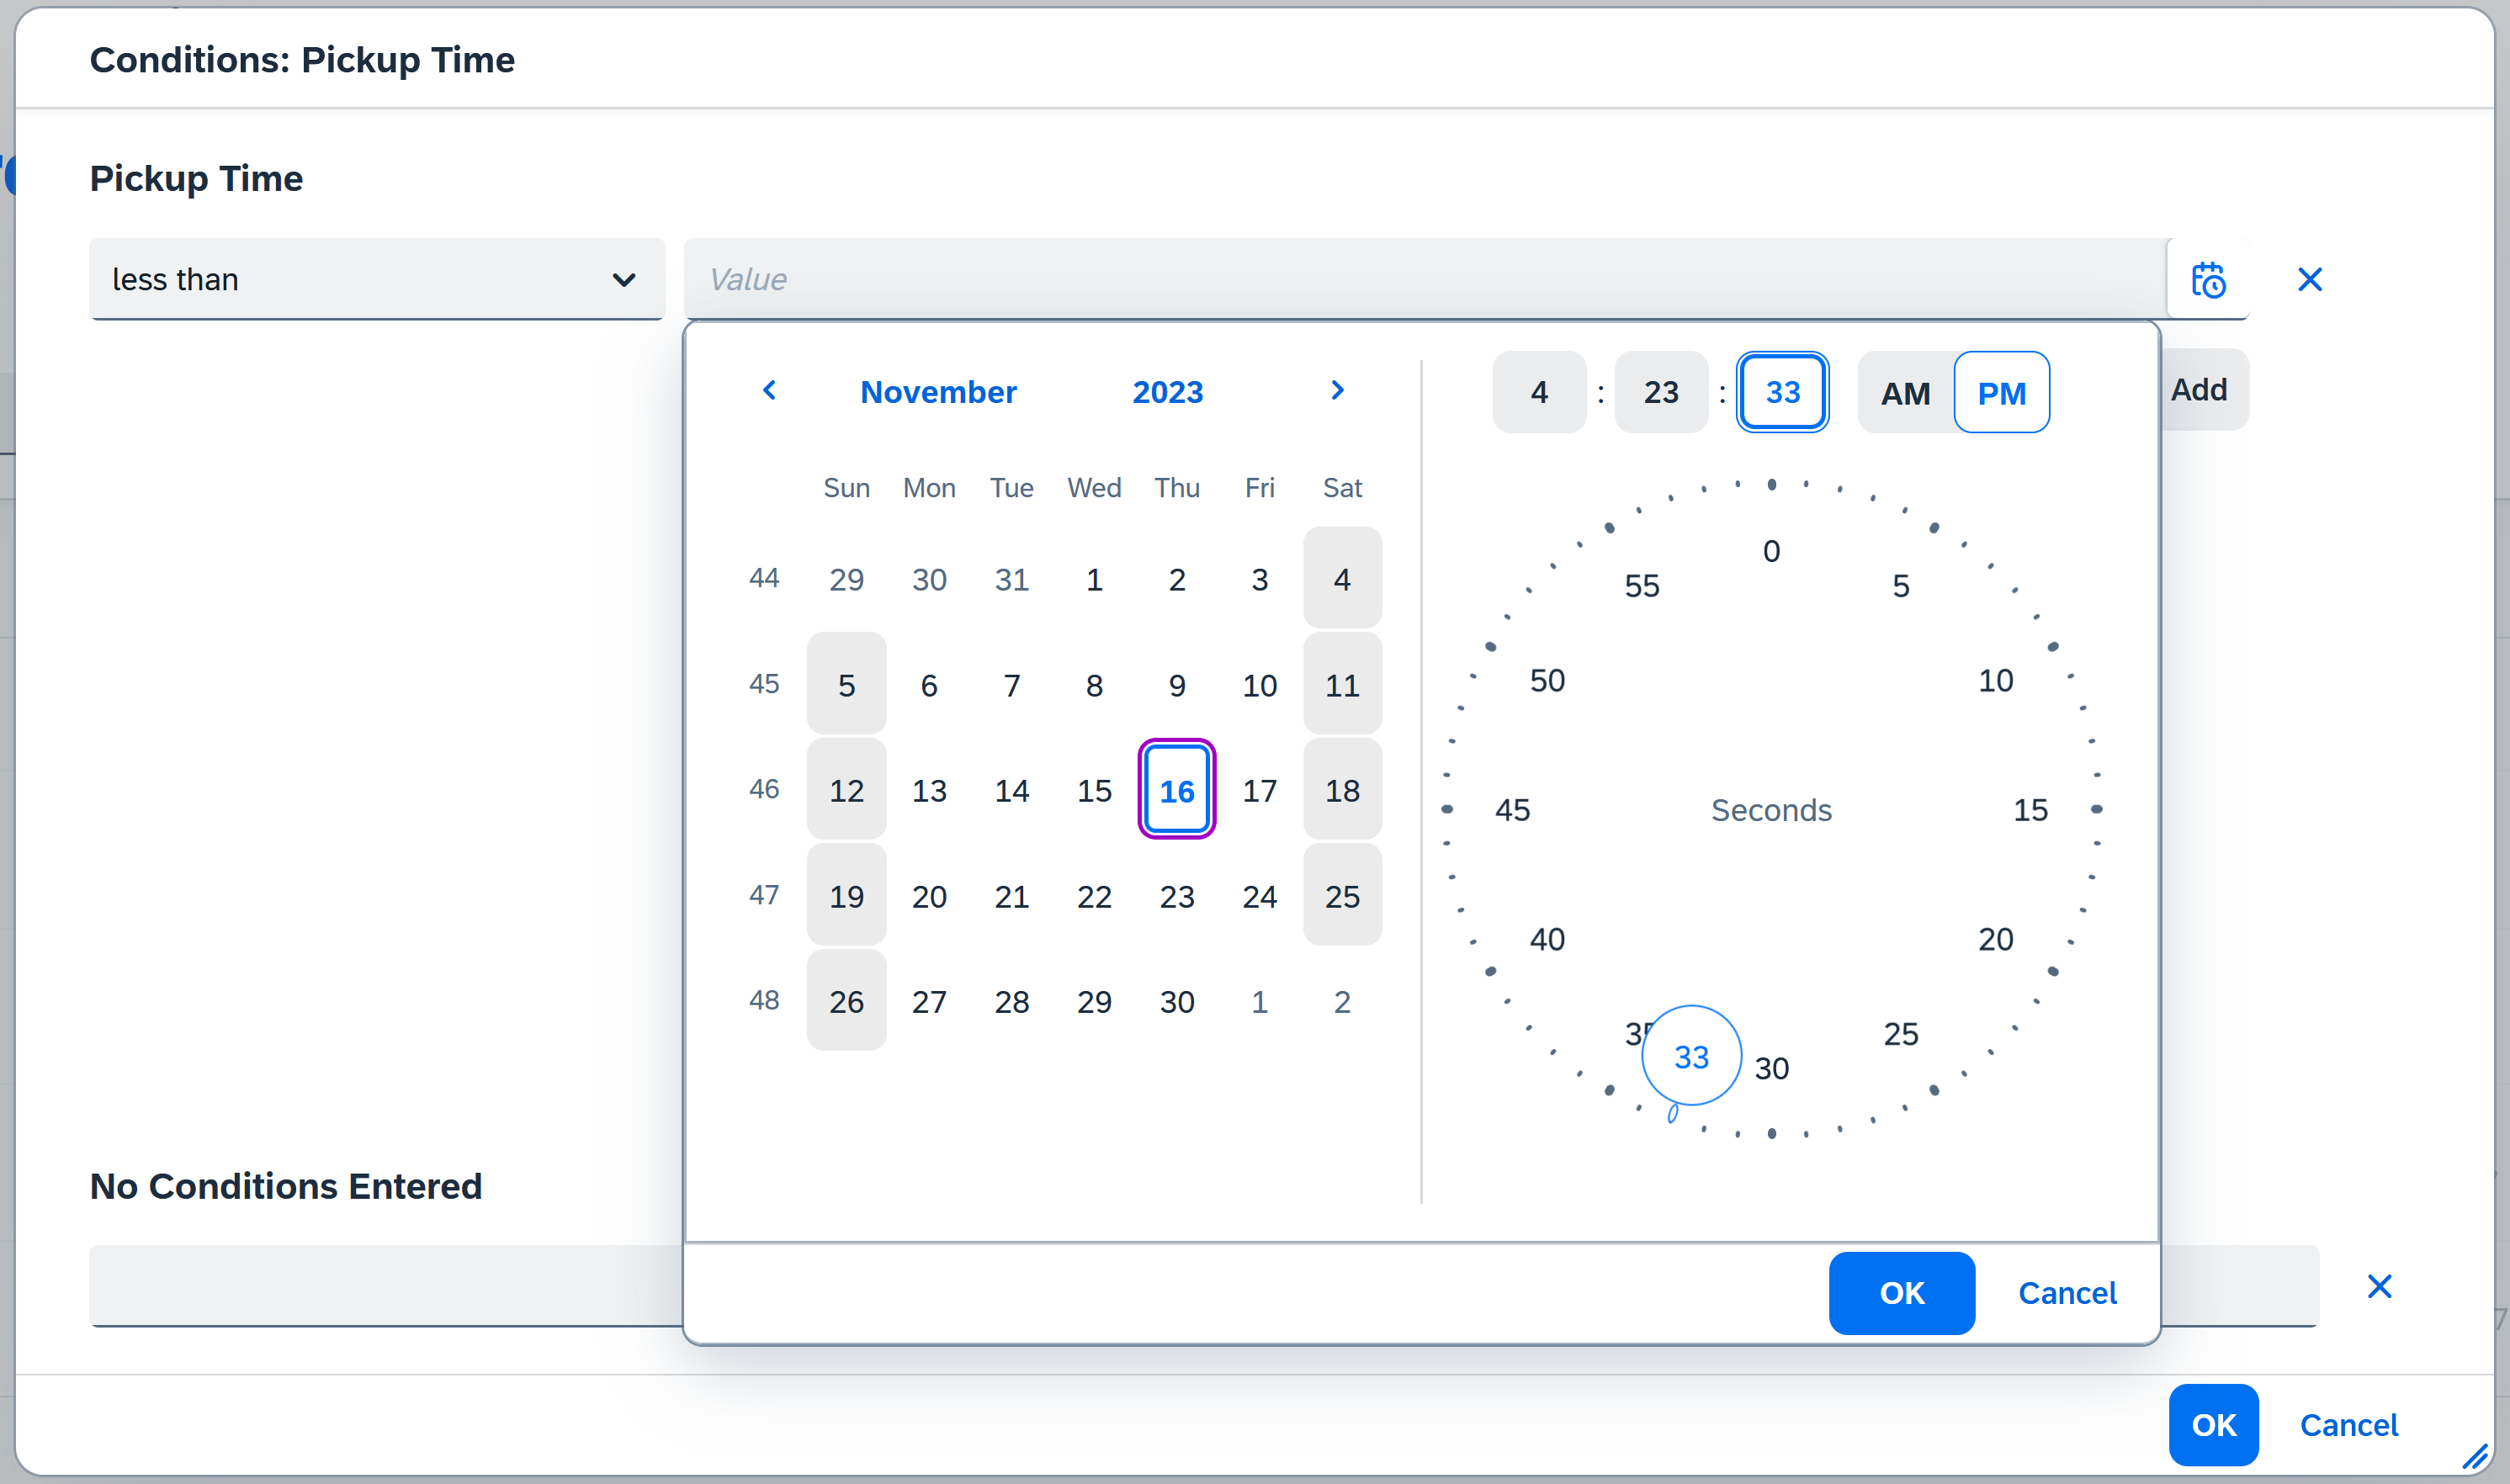
\includegraphics[width=0.45\linewidth]{images/user_doc/myPack/timeFilter-Usage2.png}}
    \caption{Time Filter Dialog - Adjust Filters}
    \label{fig:PHAjustTimeFilters}
\end{figure}


\begin{figure}[H]
		\centering
	\subcaptionbox{While Adjusting the Filter}{
		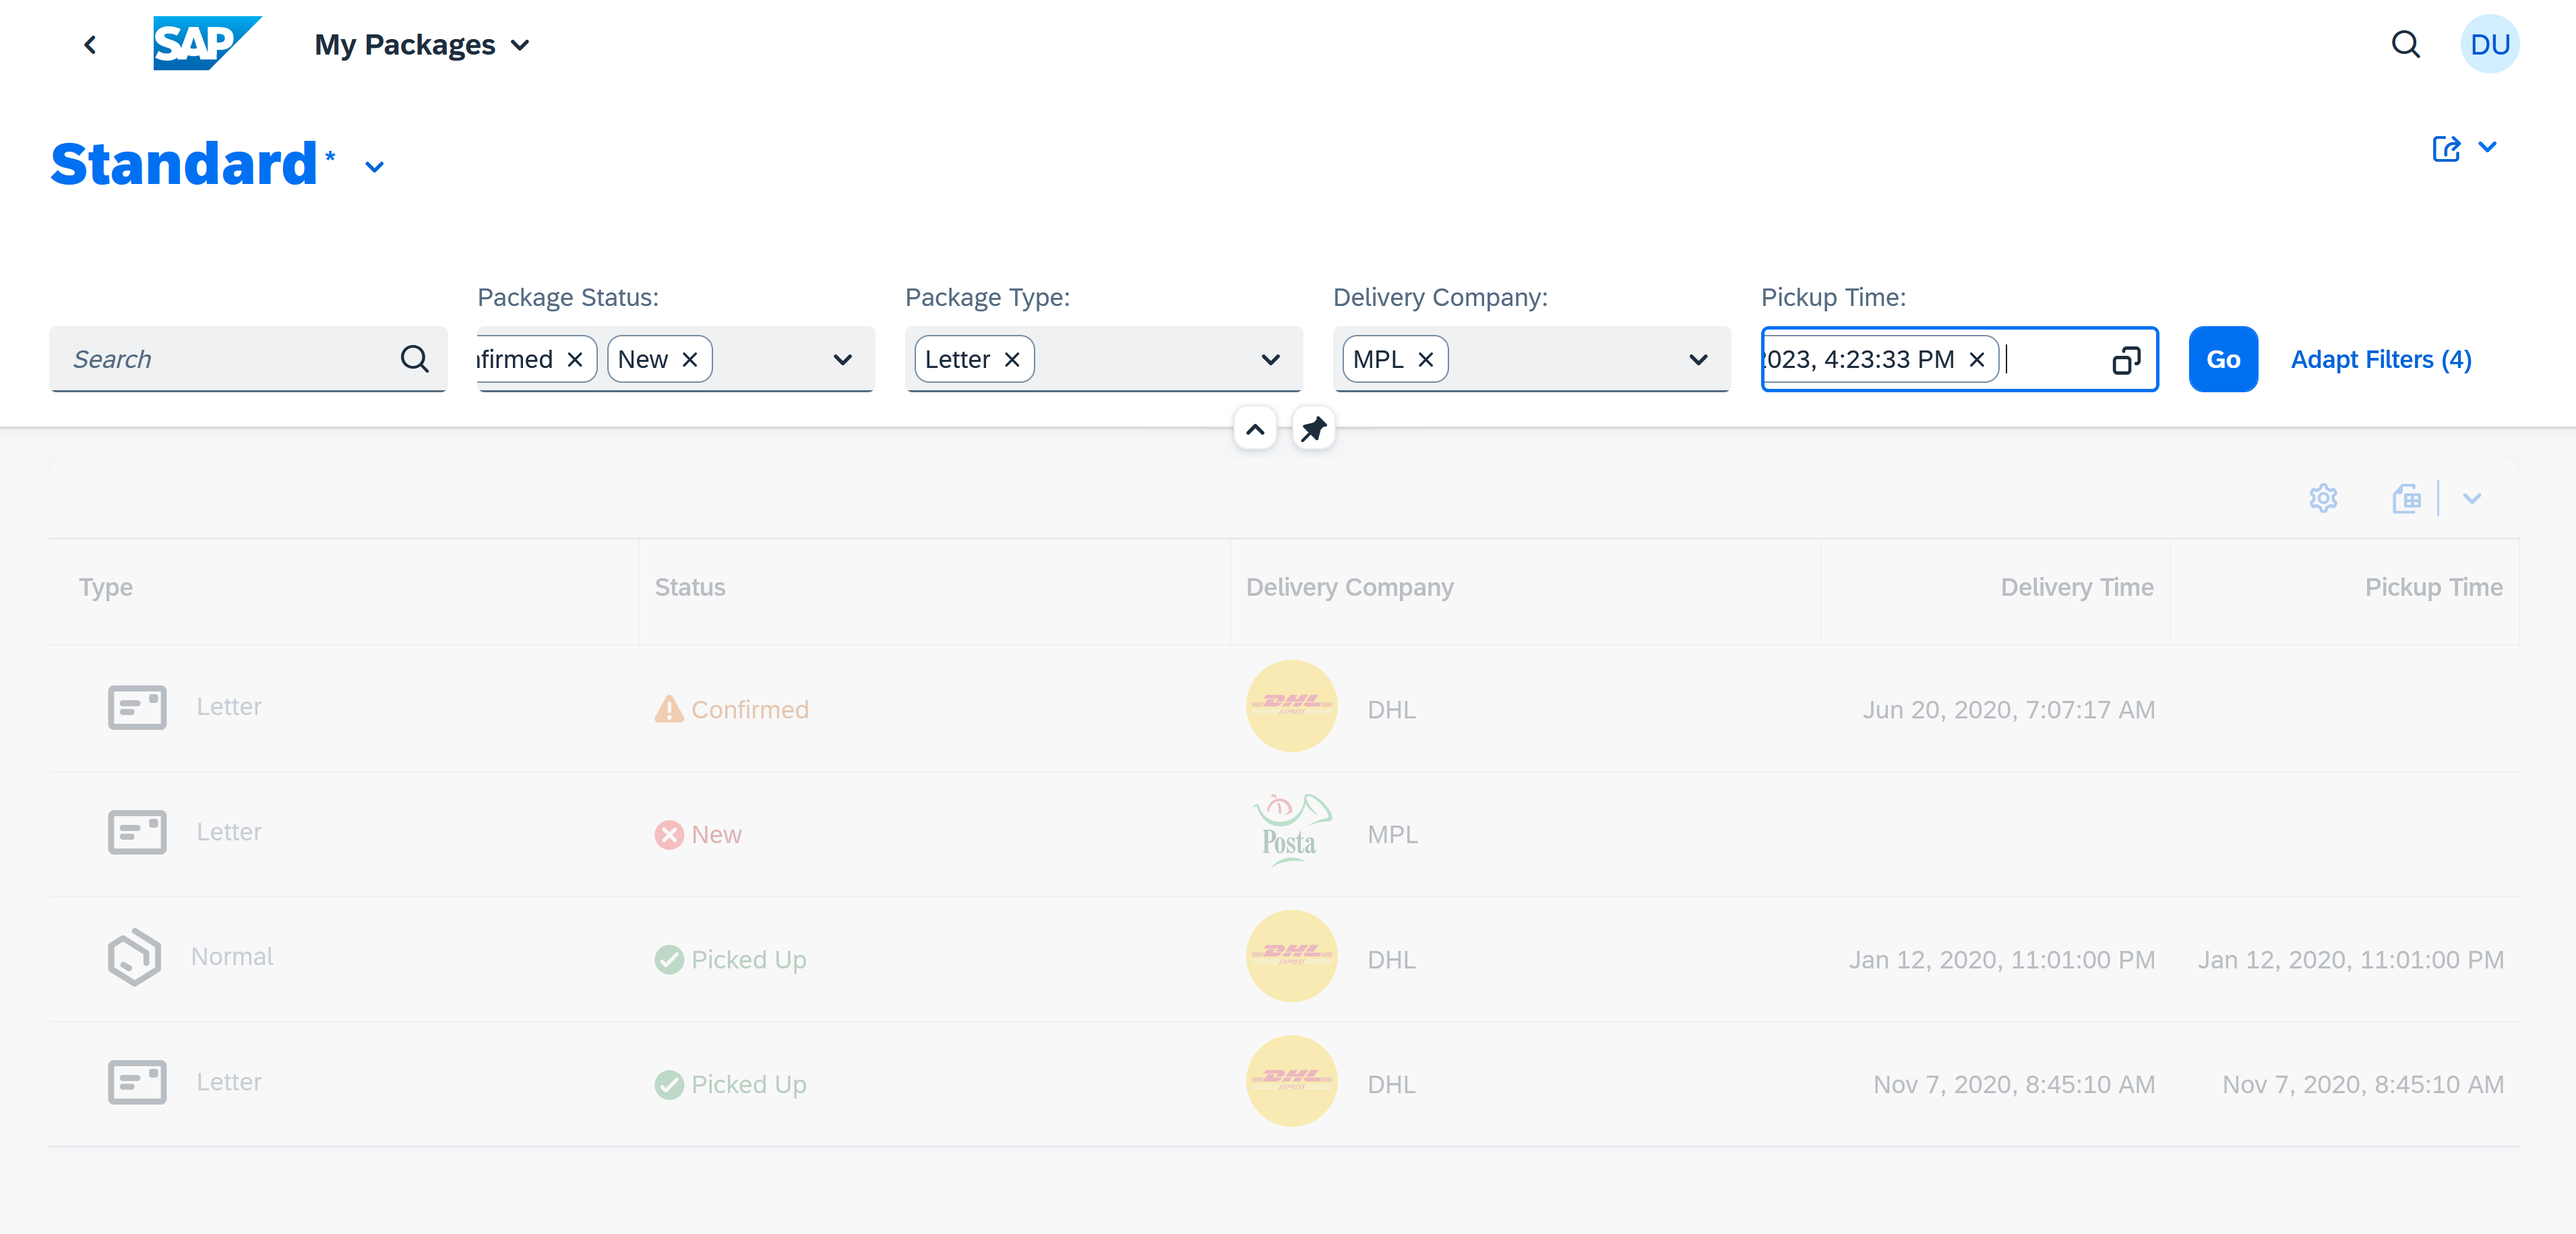
\includegraphics[width=0.45\linewidth]{images/user_doc/myPack/filterAdaptionScreen.png}}
	\hspace{5pt}
	\subcaptionbox{Clicked "Go"}{
		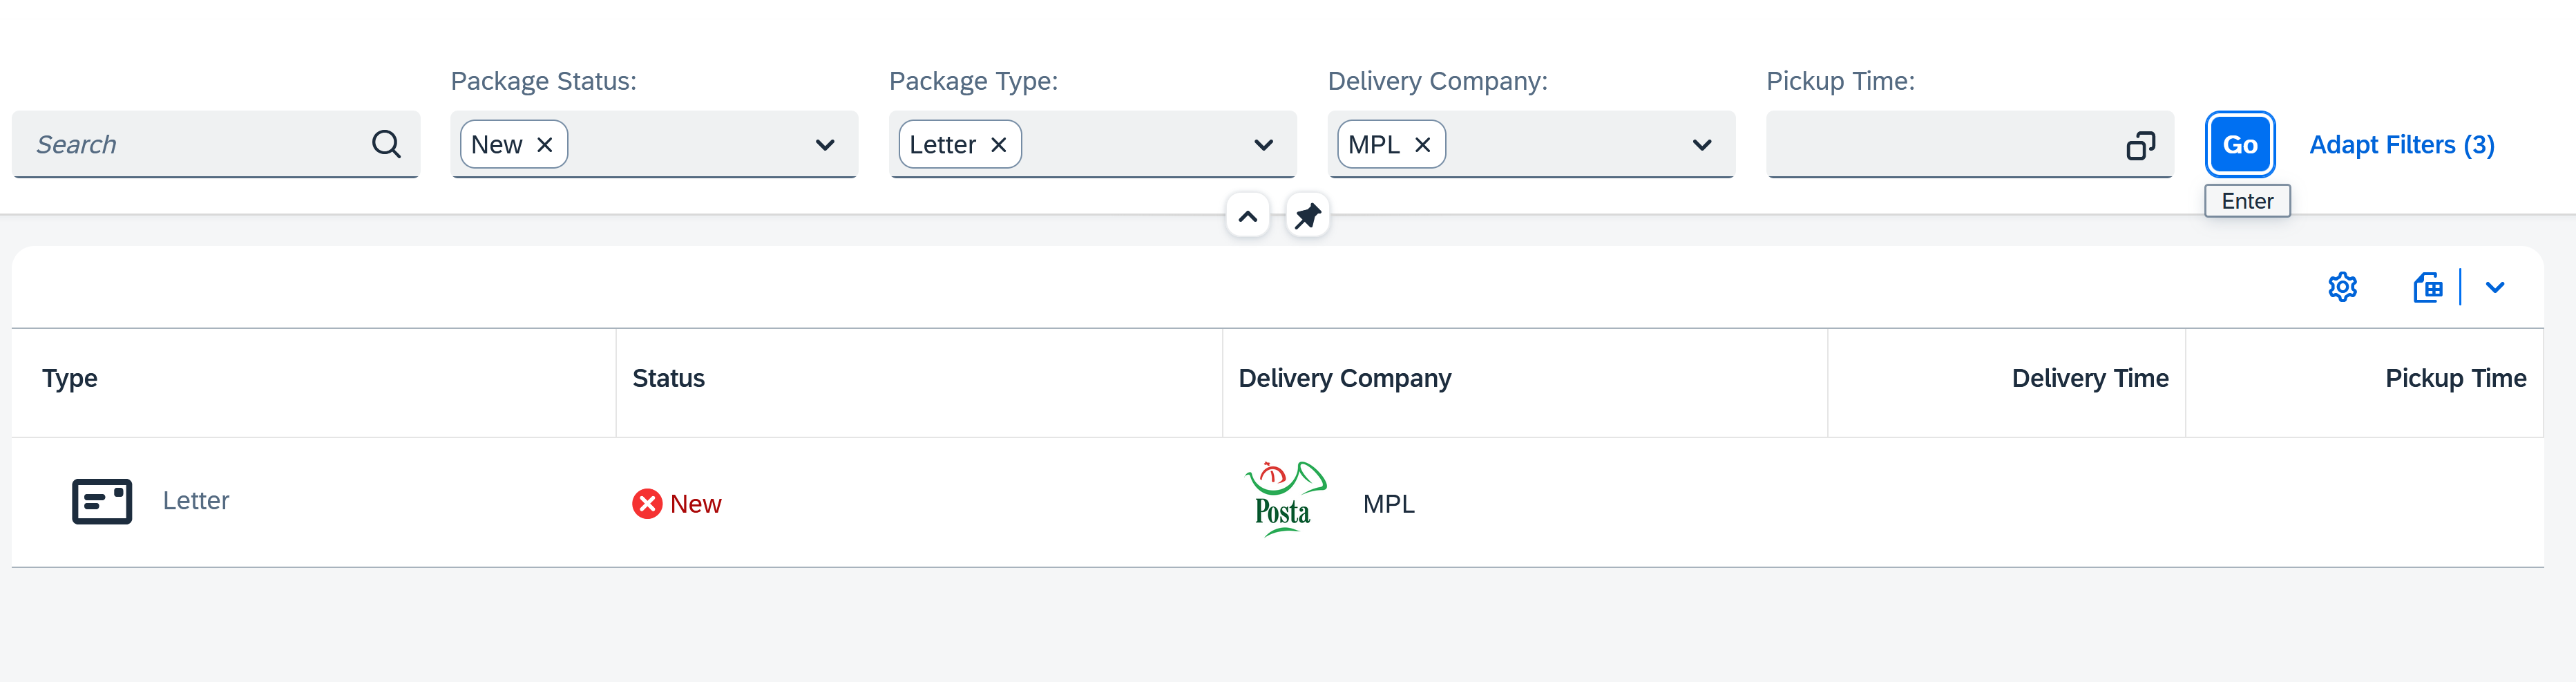
\includegraphics[width=0.45\linewidth]{images/user_doc/myPack/FilterDoneScreen.png}}
    \caption{My Package Home Screen - Adjust Filters}
    \label{fig:PHAjustFilters-2}
\end{figure}

\begin{figure}[H]
	\centering
	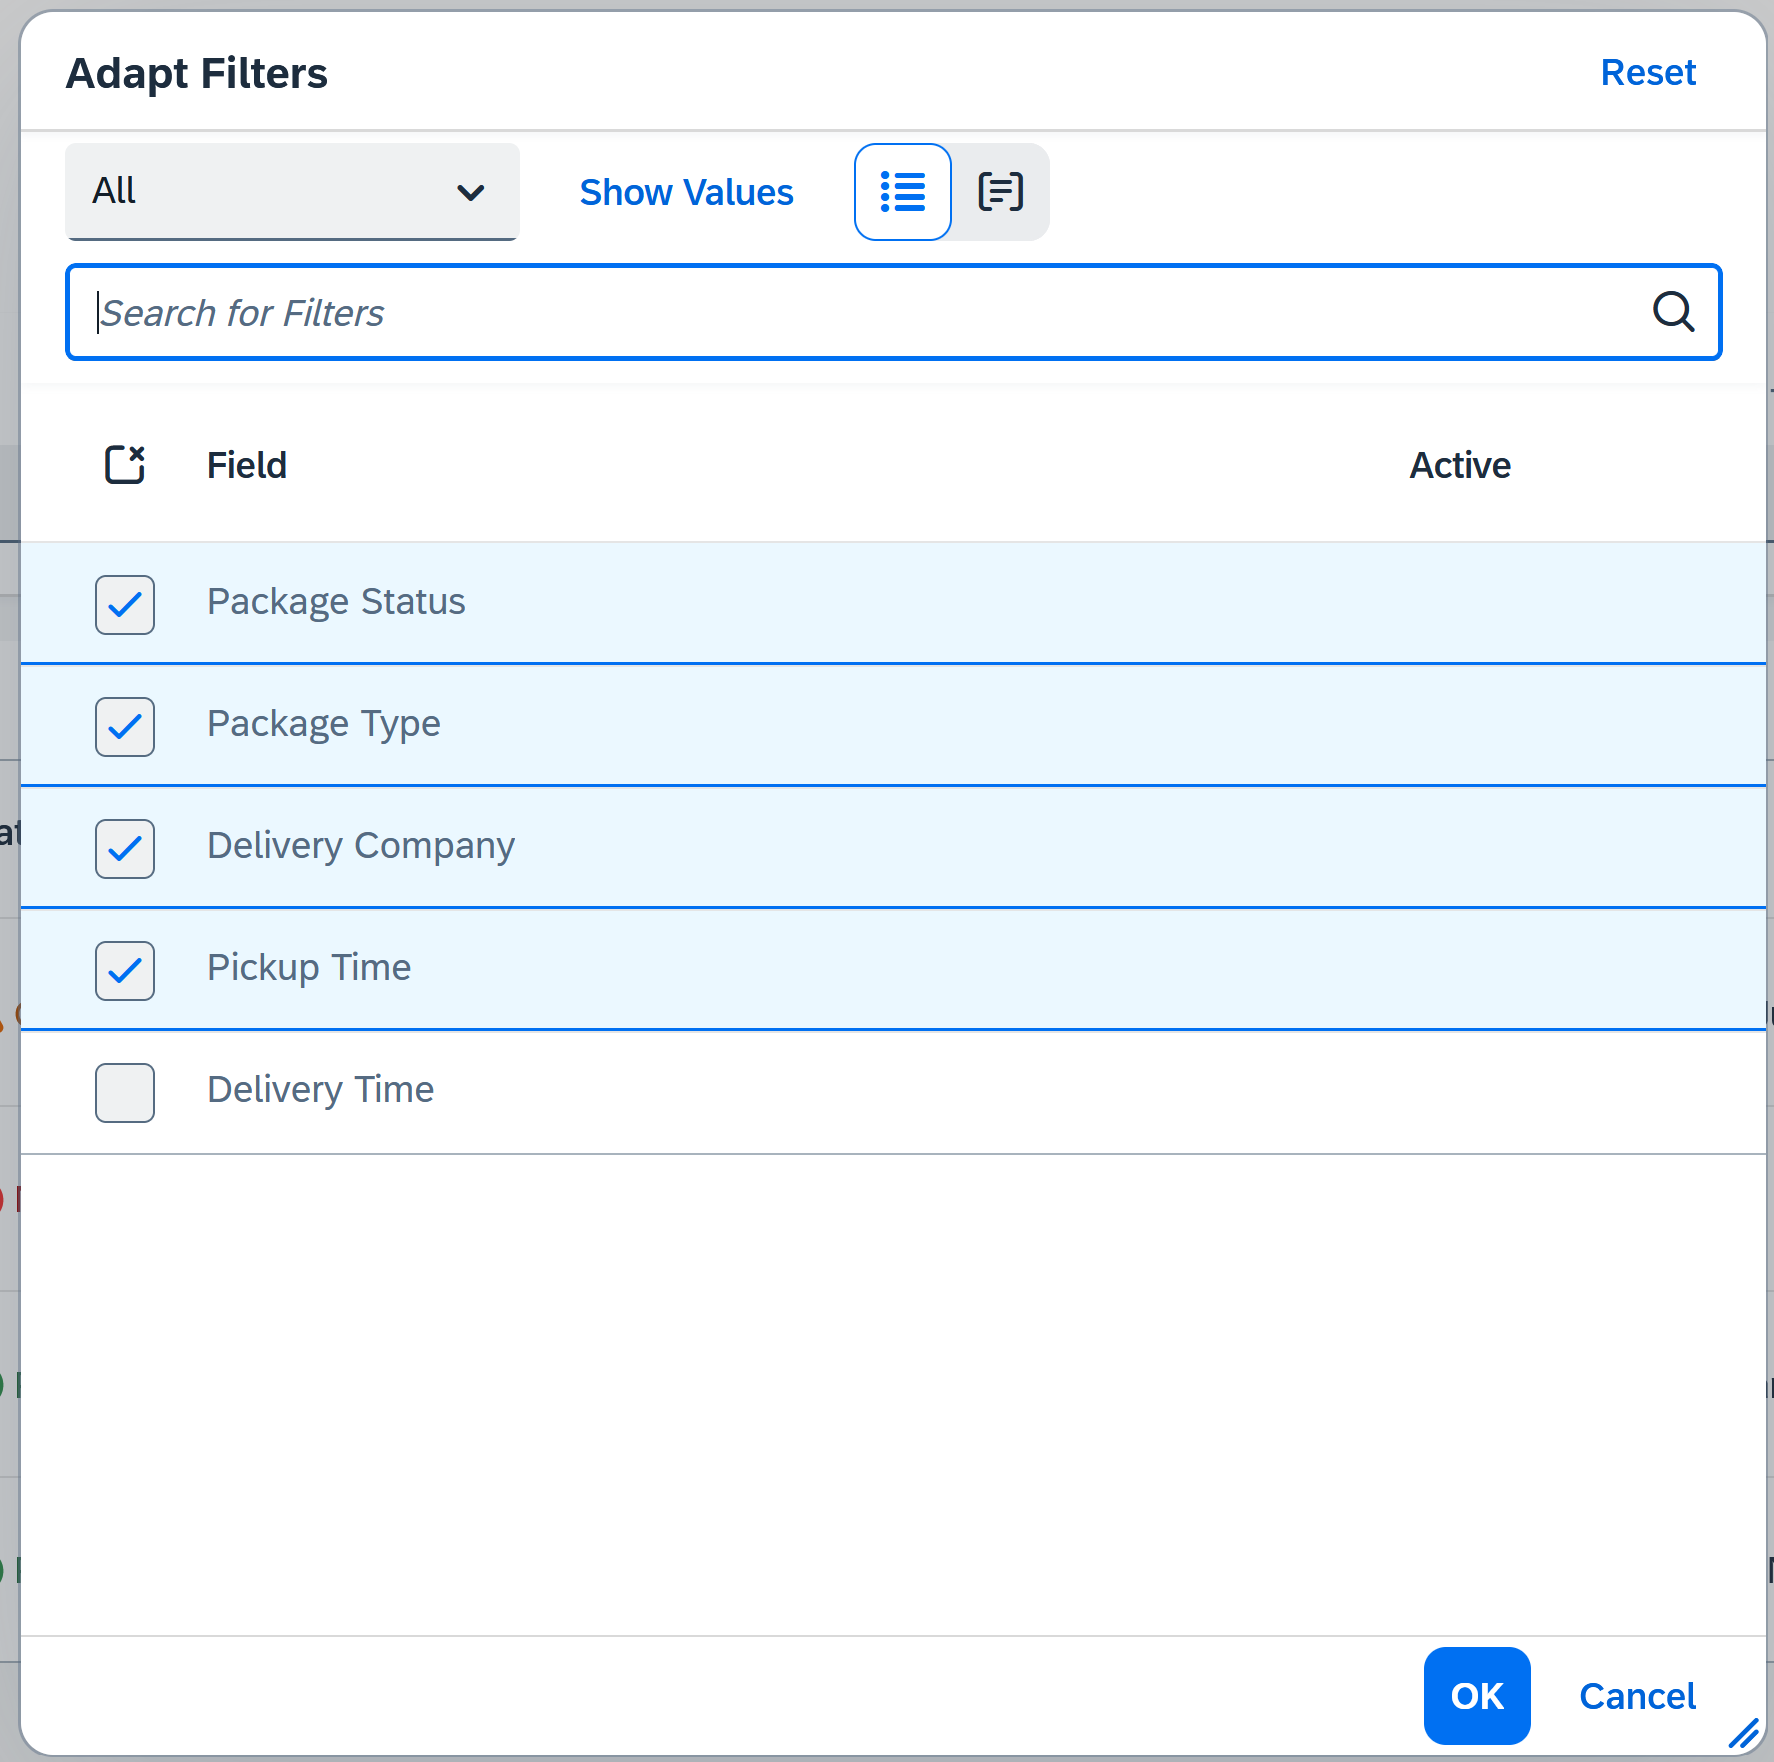
\includegraphics[height=200pt]{images/user_doc/myPack/MoreFIlterOption.png}
	\caption{My Package Filter Adaption Dialog - More Filters}
	\label{fig:mpMOreFilterAdaption}
\end{figure}
% ----------------------- Package Pickup ----------------------------
% 
%  ---------------------------------------------------------------

\subsection{Package Pickup}
\label{subsec:pp}

The \textbf{Package Pickup} application is used to pick up any confirmed parcels (registered at the reception and confirmed with a storage slot) of the logged in user. One can only see one's own confirmed packages. 
The summarized main actions the \textbf{End User} (See \autoref{sec:UdocEndUser} for all related applications) can take within the application are listed here:

\begin{compactenum}
	\item Browse the owned packages that can be picked up.
    \item Pickup the listed owned packages.
\end{compactenum}

\bigskip
\textbf{Hint}: The application supports only from mobile devices. In case an employee is unable to access his or her mobile at the moment of pickup, he or she shall ask the receptionist to pickup the package for him or her.


\subsubsection{Home Screen - Selection}
As an \textbf{End User}, after clicking at the application tile, is redirected to the "Home Screen". If there exists at least one package to pickup, the home screen shows the list of packages. 
The list items lists \textbf{the type with icon, the delivery company, the registration time and the location} of the packages. 
If no package exists to pickup, it shows only the no package info. 
The package list title shows the total number of packages that can be pickup.
In case there are existing packages, one can select one or multiple packages from the list to pickup. 
In case there are existing packages, one can tick/untick the "Toggle All" selection box to select or deselect the package all at once. 
(\autoref{fig:PickupHomeScreen-1}, \autoref{fig:PickupHomeScreen-2})

\begin{figure}[H]
	\centering
	\subcaptionbox{Home Screen with Packages}{
		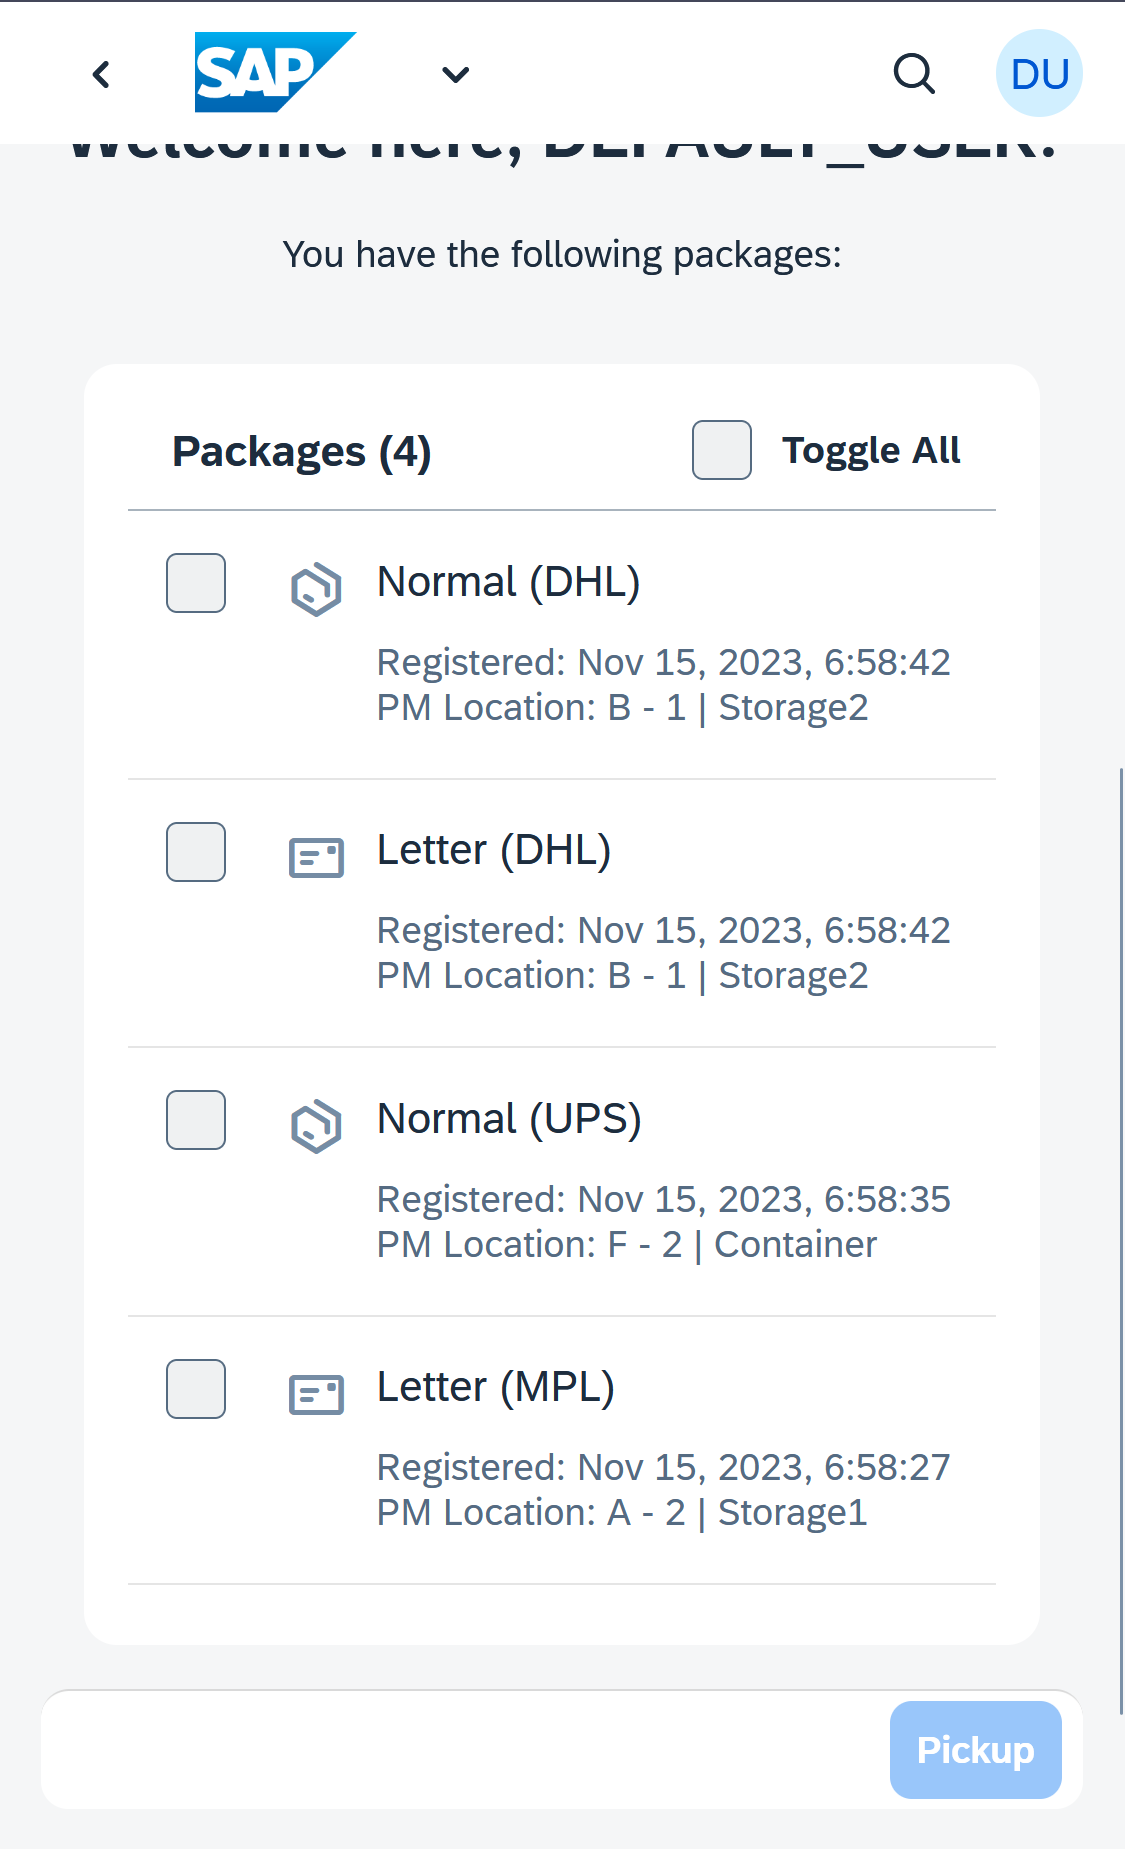
\includegraphics[width=0.45\linewidth]{images/user_doc/pickup/HomeScreenList.png}}
	\hspace{5pt}
	\subcaptionbox{Home Screen without Packages}{
		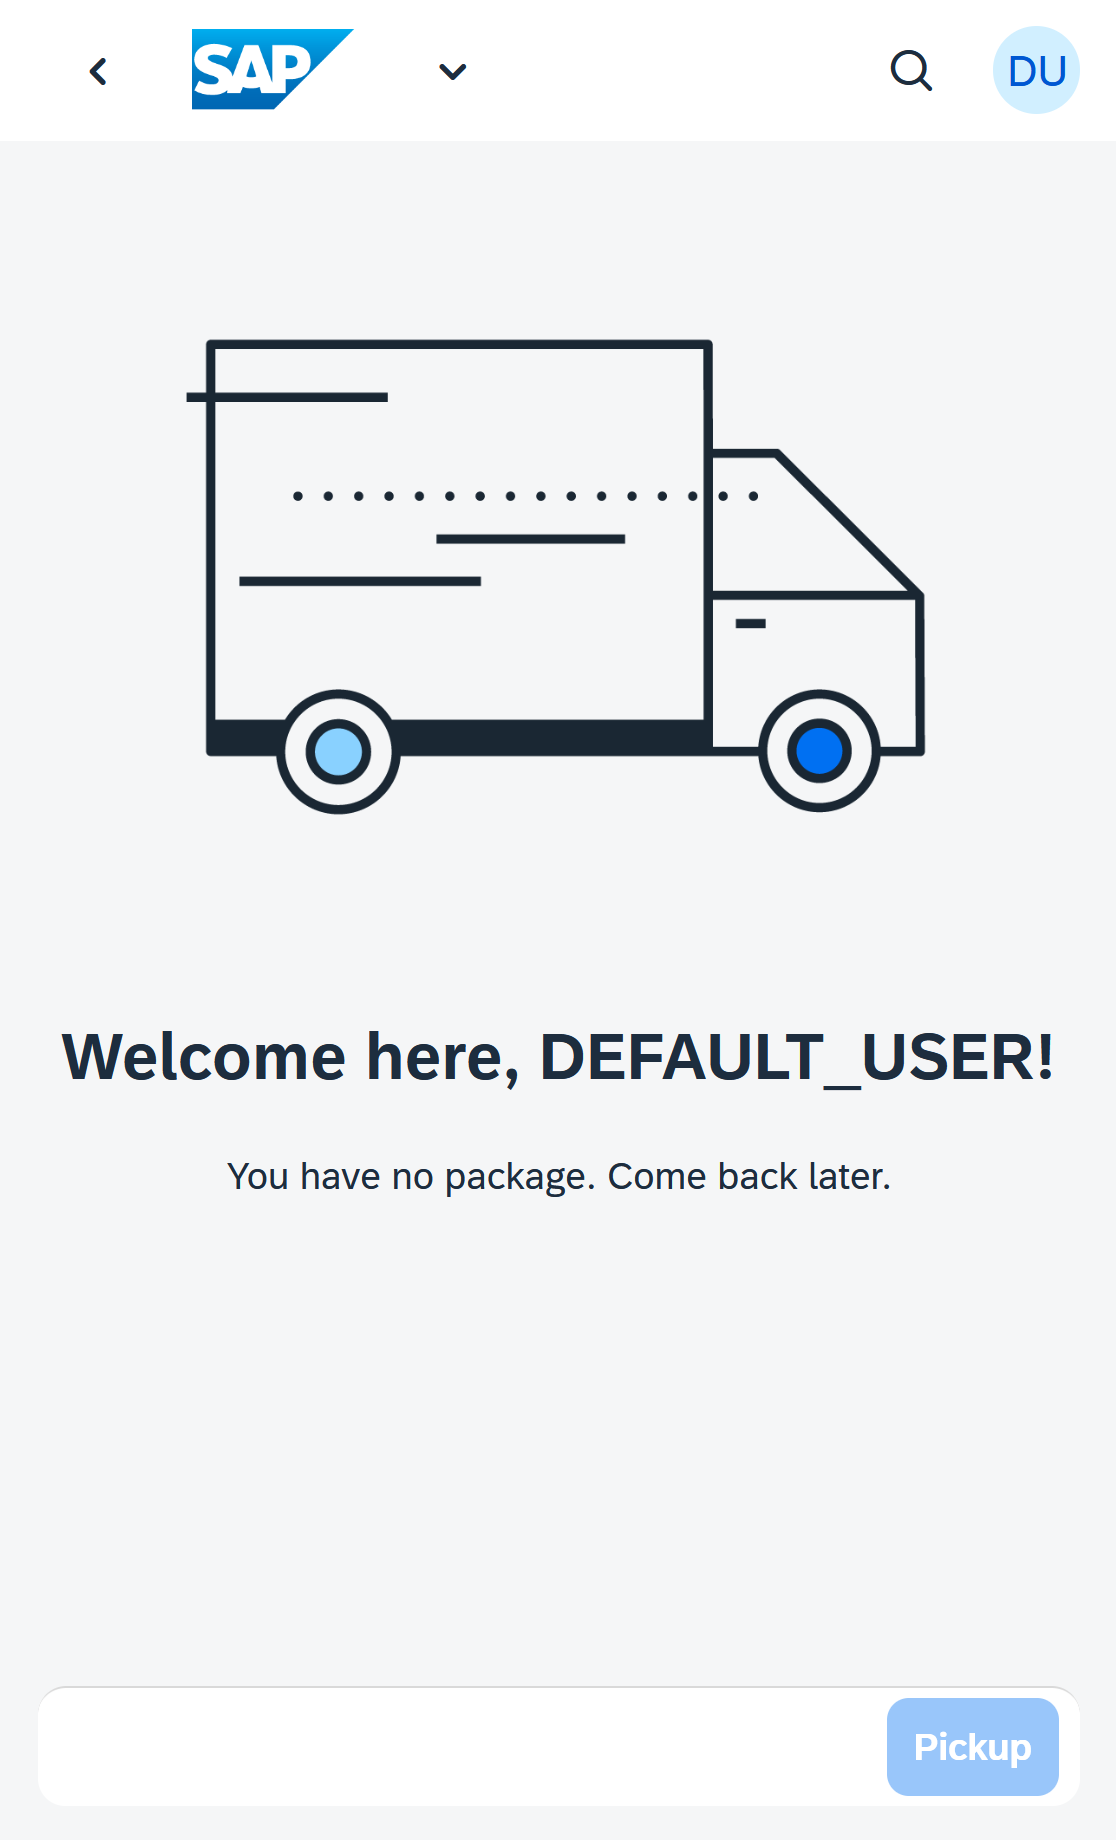
\includegraphics[width=0.45\linewidth]{images/user_doc/pickup/HomeScreenNoPackage.png}}
	\caption{Pickup Home Screen - Package Existence Guide}
	\label{fig:PickupHomeScreen-1}
\end{figure}

\begin{figure}[H]
	\centering
	\subcaptionbox{Home Screen Single Selection}{
		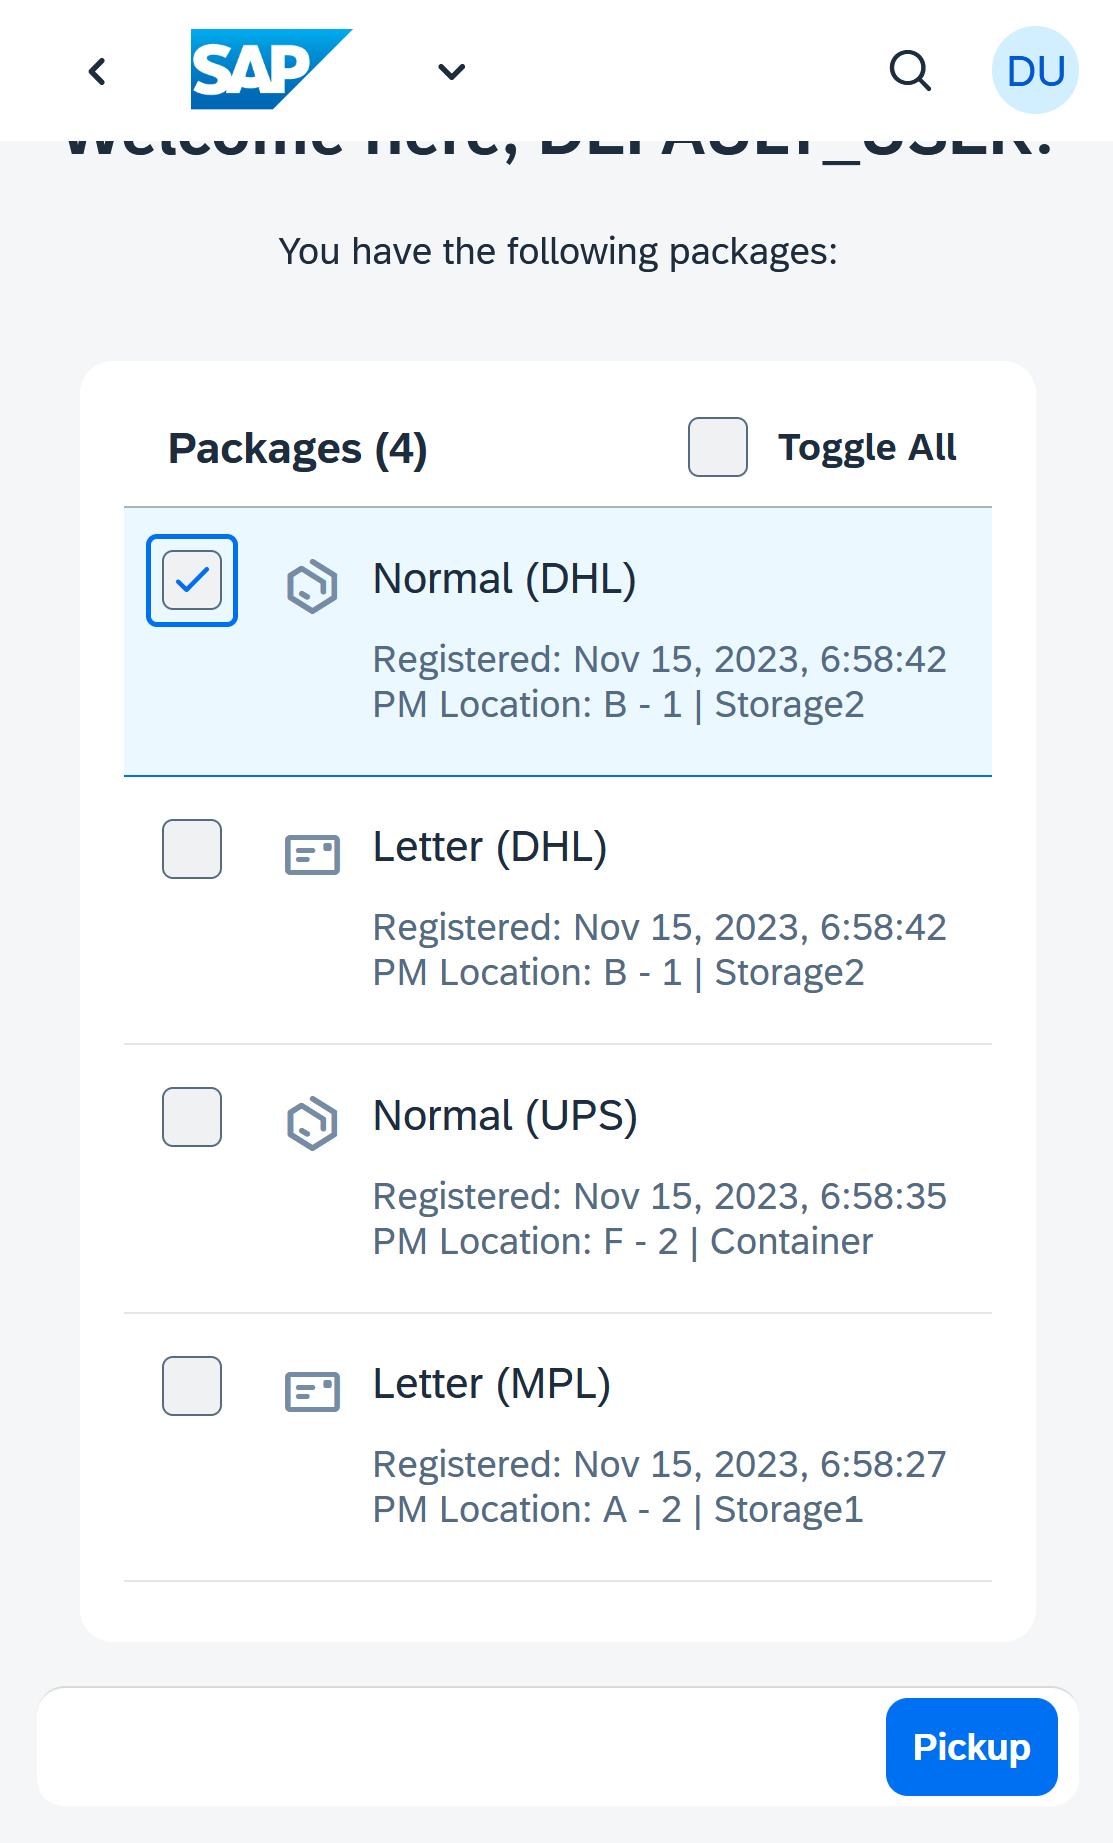
\includegraphics[width=0.45\linewidth]{images/user_doc/pickup/HomeScreenSelectOne.png}}
	\hspace{5pt}
	\subcaptionbox{Home Screen Multiple Selection}{
		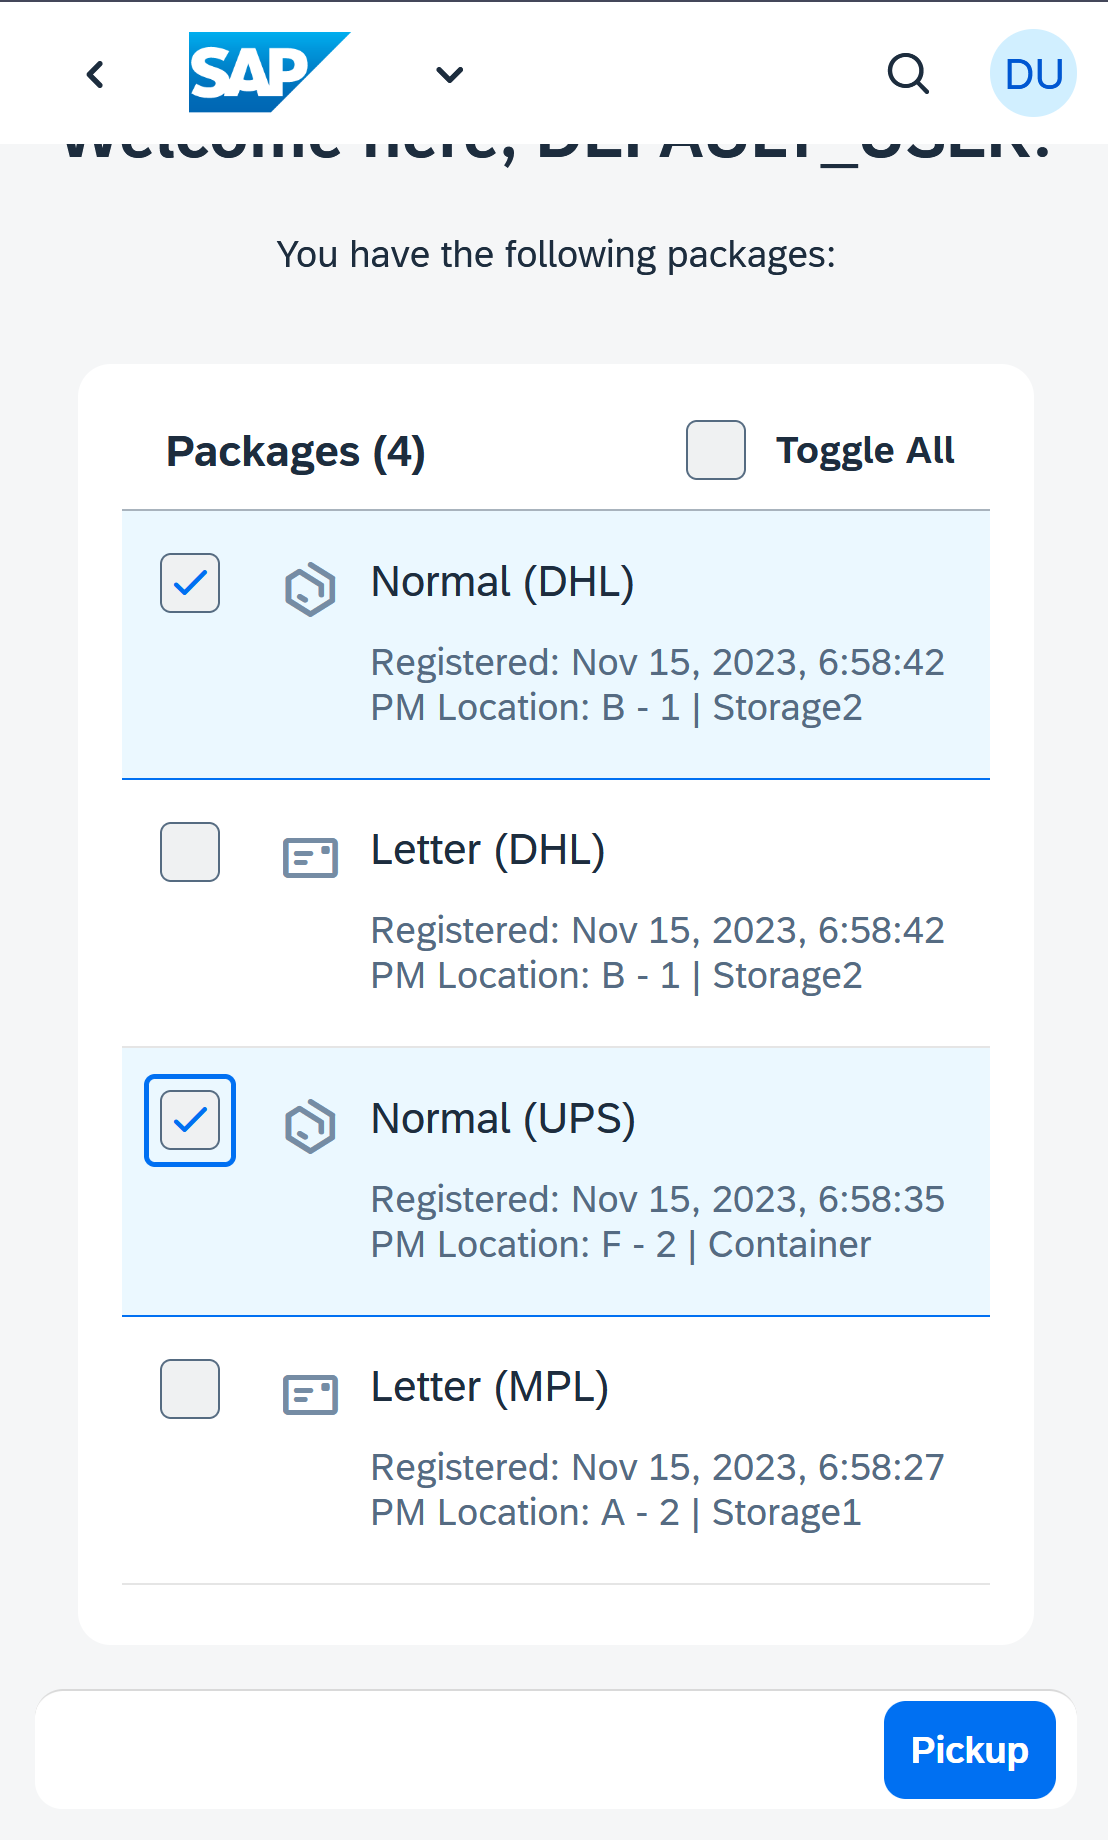
\includegraphics[width=0.45\linewidth]{images/user_doc/pickup/HomeScreenMultiSelect.png}}

    \subcaptionbox{Home Screen Select All}{
		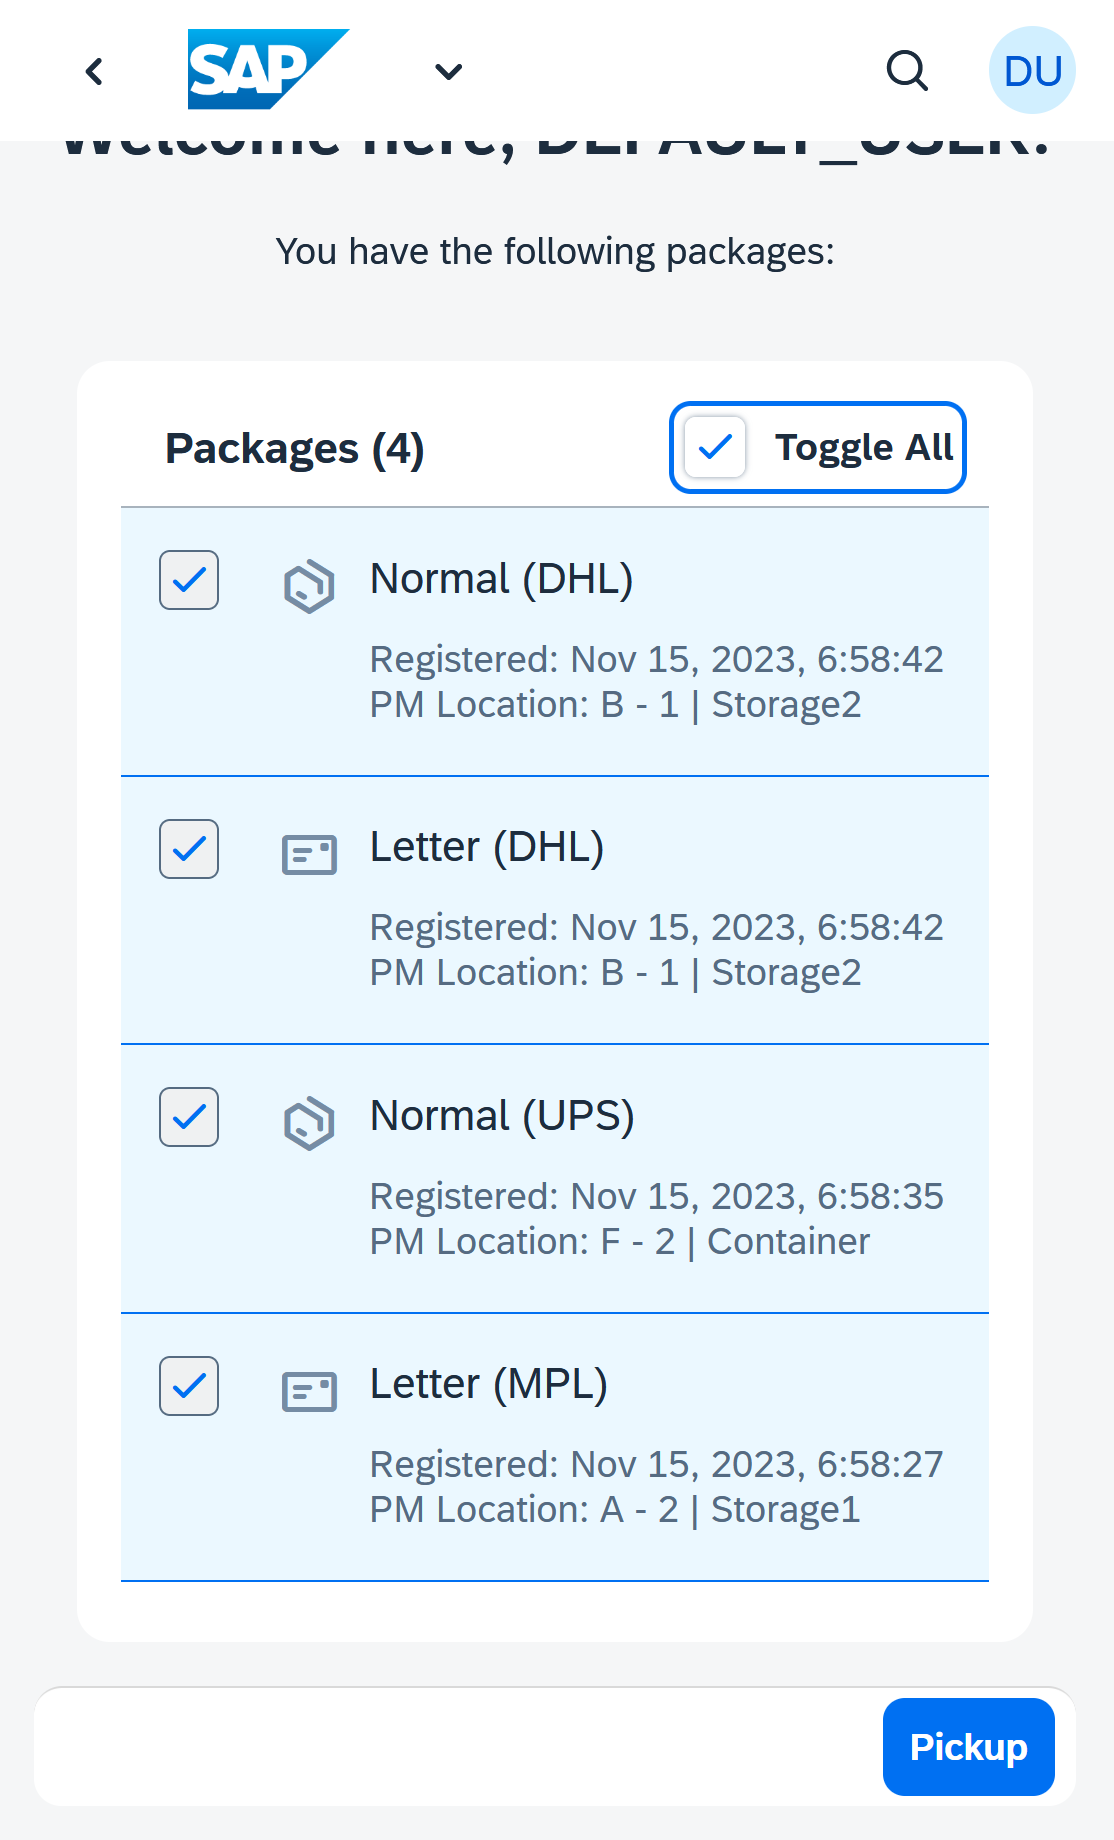
\includegraphics[width=0.45\linewidth]{images/user_doc/pickup/HomeScreenToggleAll.png}}
	\hspace{5pt}
	\subcaptionbox{Home Screen Deselect All}{
		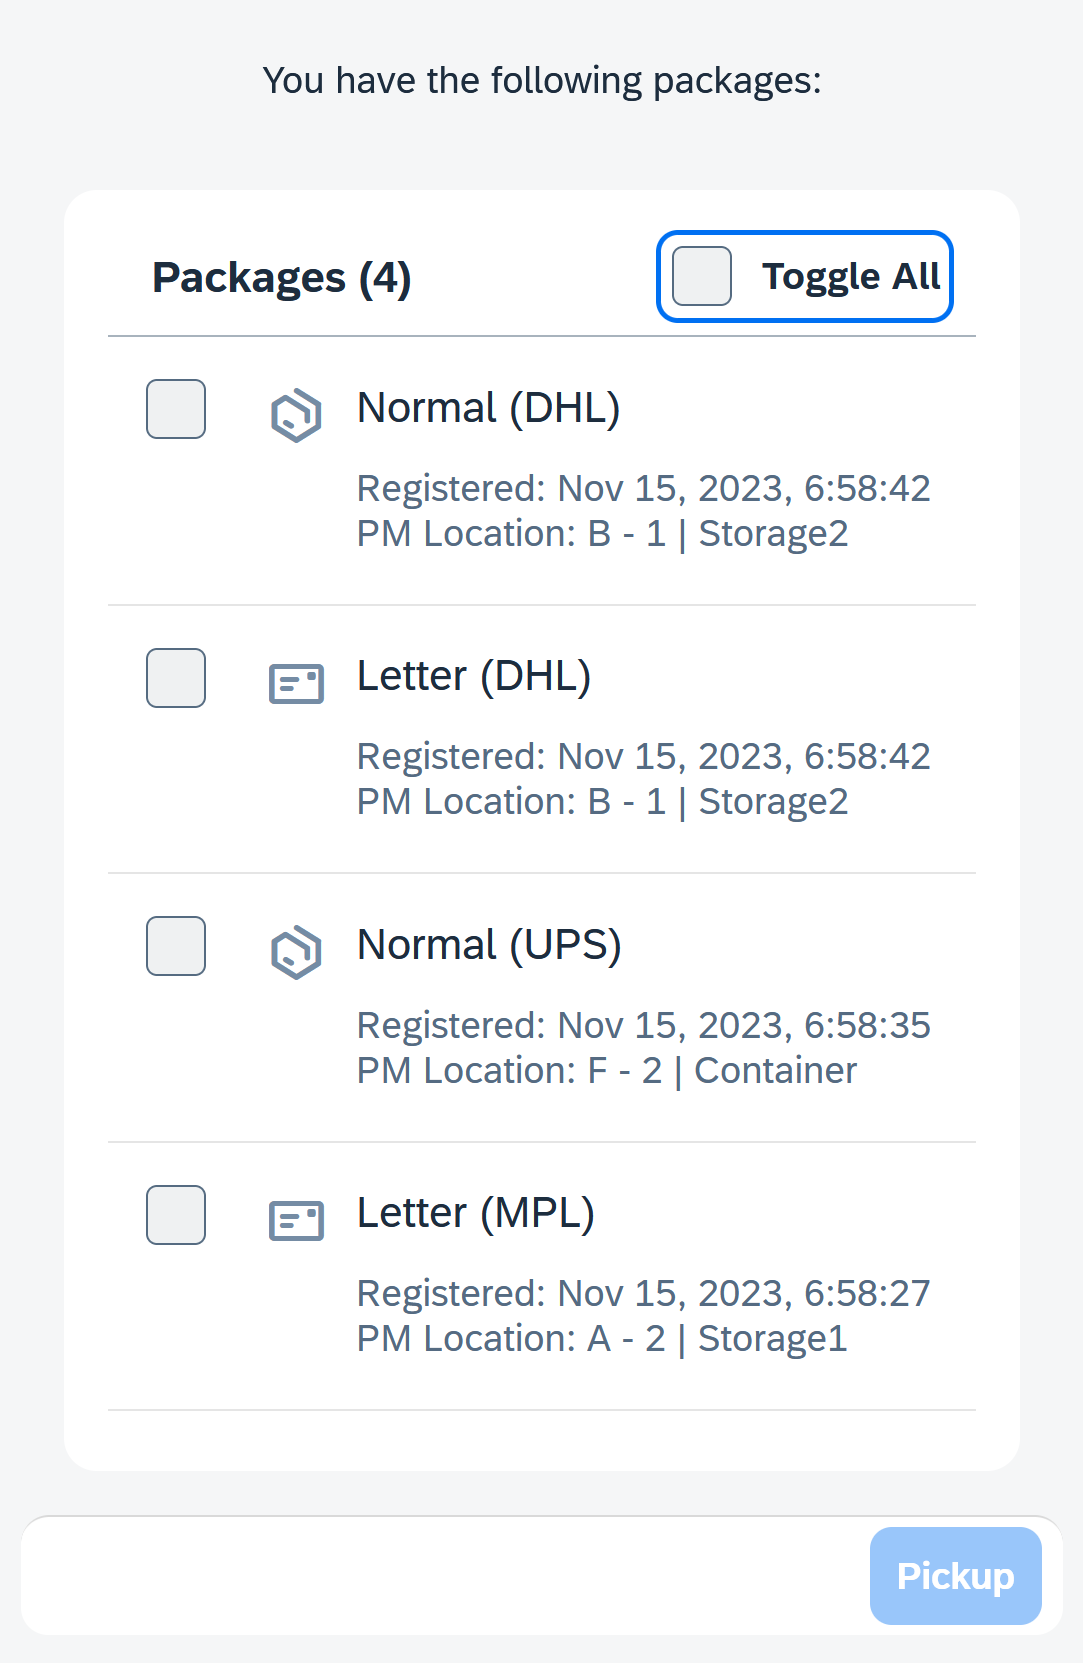
\includegraphics[width=0.45\linewidth]{images/user_doc/pickup/HomeScreenDeToggleAll.png}}
	\caption{Pickup Home Screen - Package Selection Guide}
	\label{fig:PickupHomeScreen-2}
\end{figure}


\subsubsection{Home Screen - Pickup}
The "Pickup" button at right bottom corner will only be enabled if at least one package is selected. In case it is enabled, one can pick up the selected packages by left clicking the "Pickup" button, which will trigger a confirmation dialog. If one choose "Cancel", the dialog closes and no modification is made. If one choose "OK", then all packages selected will be marked as pickup, removed from the list and the user will be navigated to the "Done Screen". At this point, the process of the picked up package will be closed, the package data will never be deleted and \textbf{End User} can always go to \textbf{My Packages} application to check the package history. (figure \ref{fig:PickupDialog})

\begin{figure}[H]
	\centering
	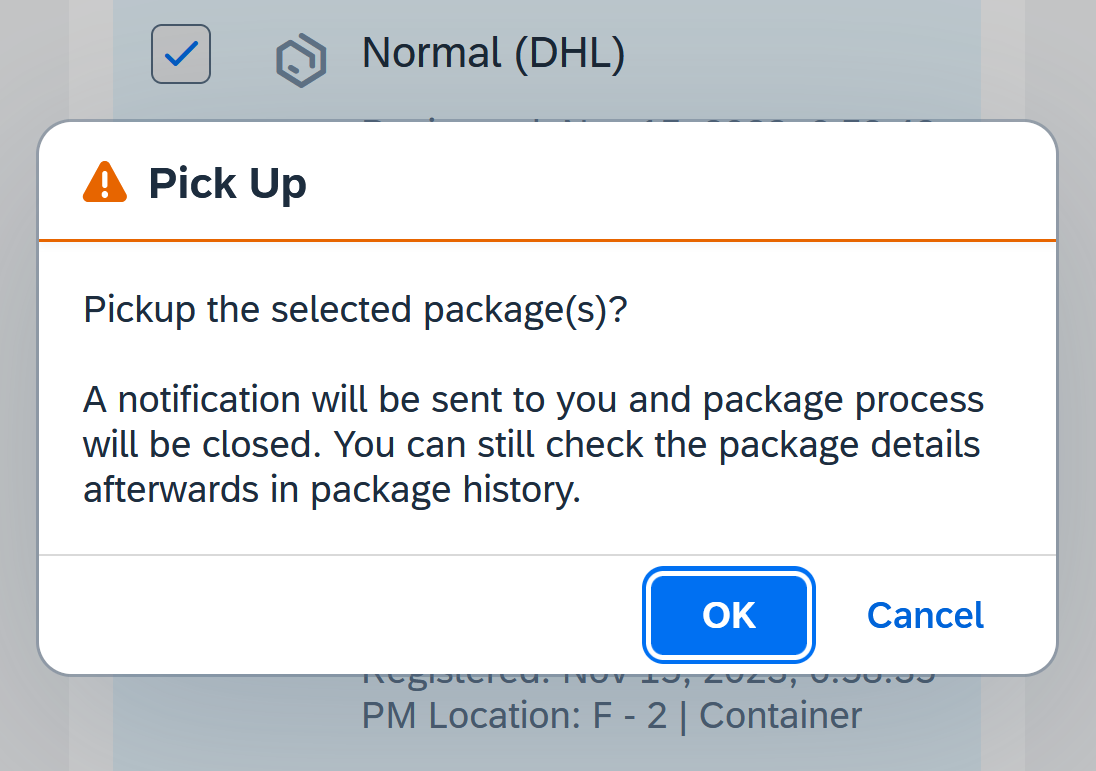
\includegraphics[height=200pt]{images/user_doc/pickup/PickupDialog.png}
	\caption{Pickup Home Screen - Pickup Dialog}
	\label{fig:PickupDialog}
\end{figure}


\subsubsection{Done Screen}

At the "Done Screen", if the \textbf{End User} still have packages to pickup, it will display the list of packages showing their \textbf{type with icon}, \textbf{delivery company} and \textbf{location info}. Otherwise, it displays no more packages. 
User can always navigate back to "Home Screen" by left clicking the "Close" button at the right bottom corner of the page.
From there, a new pickup iteration starts.
(figure \ref{fig:PickupDoneScreen-1})

\begin{figure}[H]
	\centering
	\subcaptionbox{Done Screen with Packages}{
		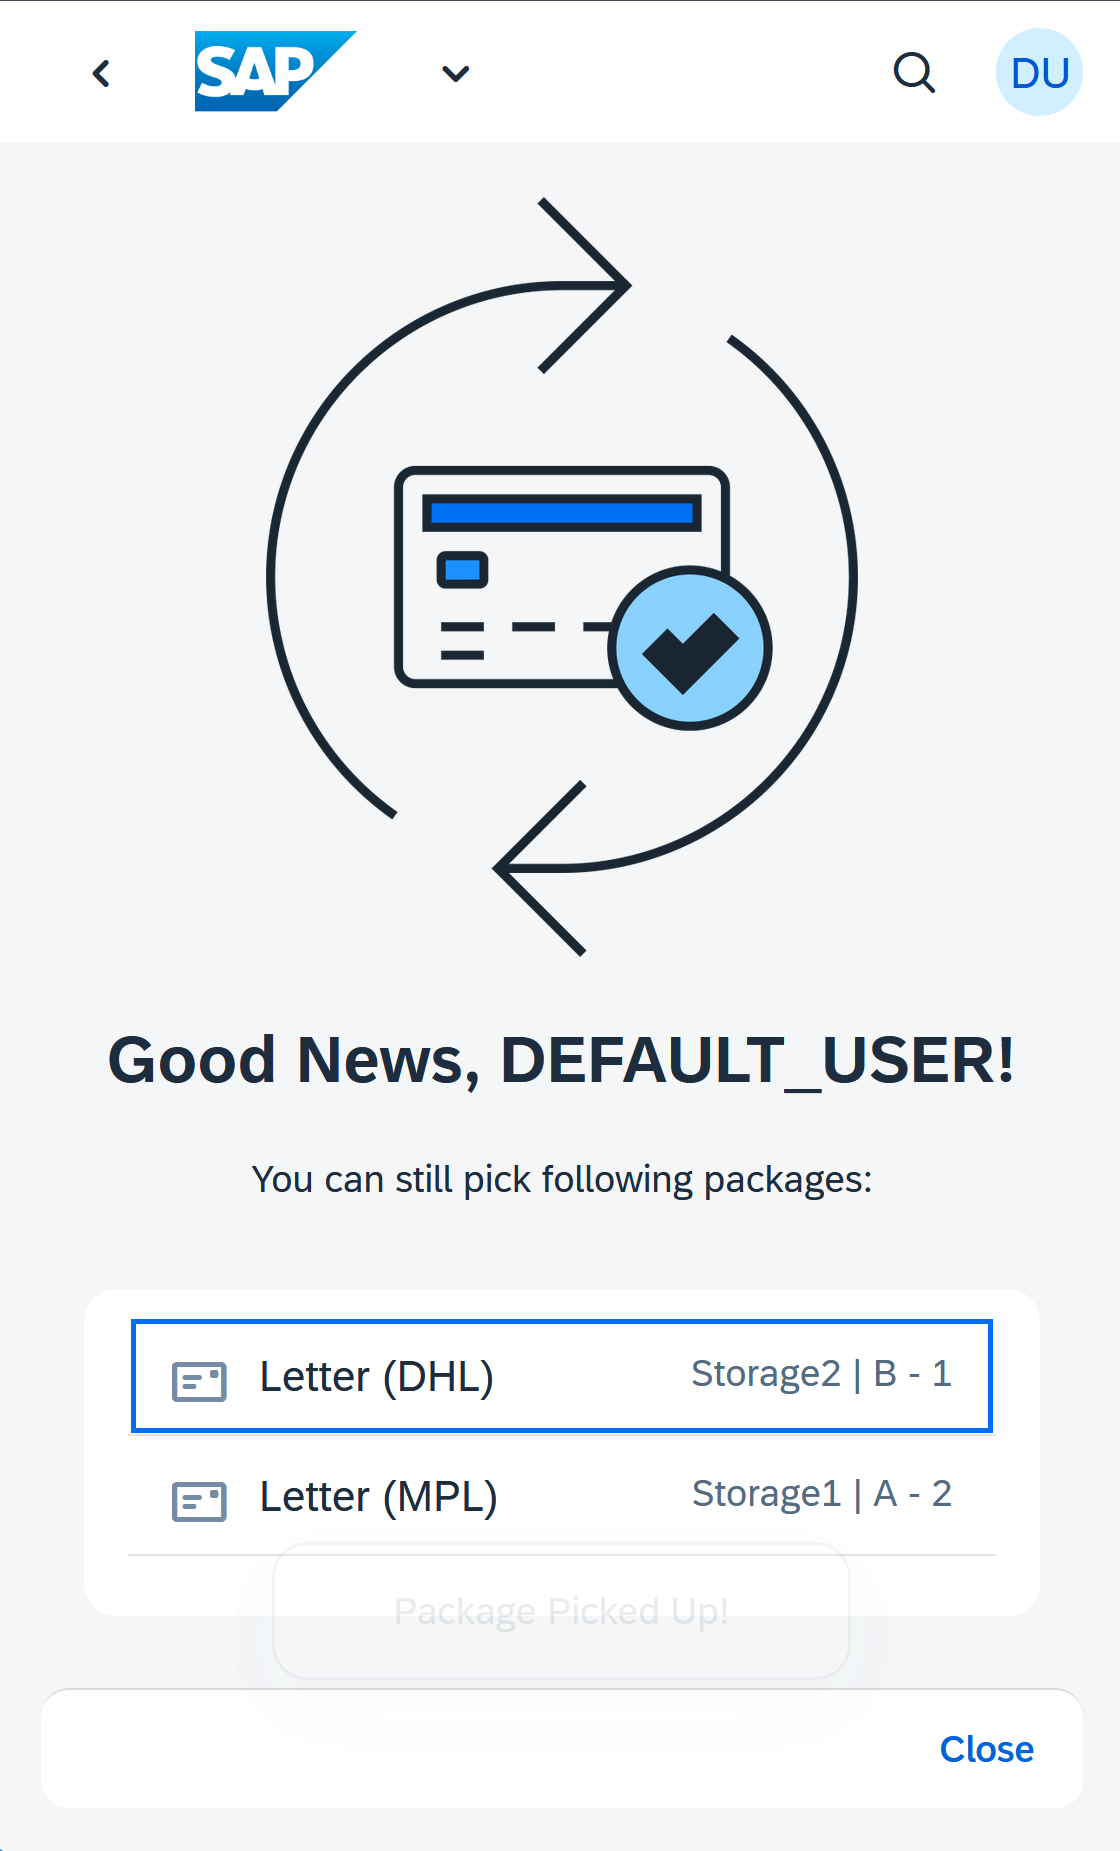
\includegraphics[width=0.45\linewidth]{images/user_doc/pickup/DoneScreenRemainPackages.png}}
	\hspace{5pt}
	\subcaptionbox{Done Screen without Packages}{
		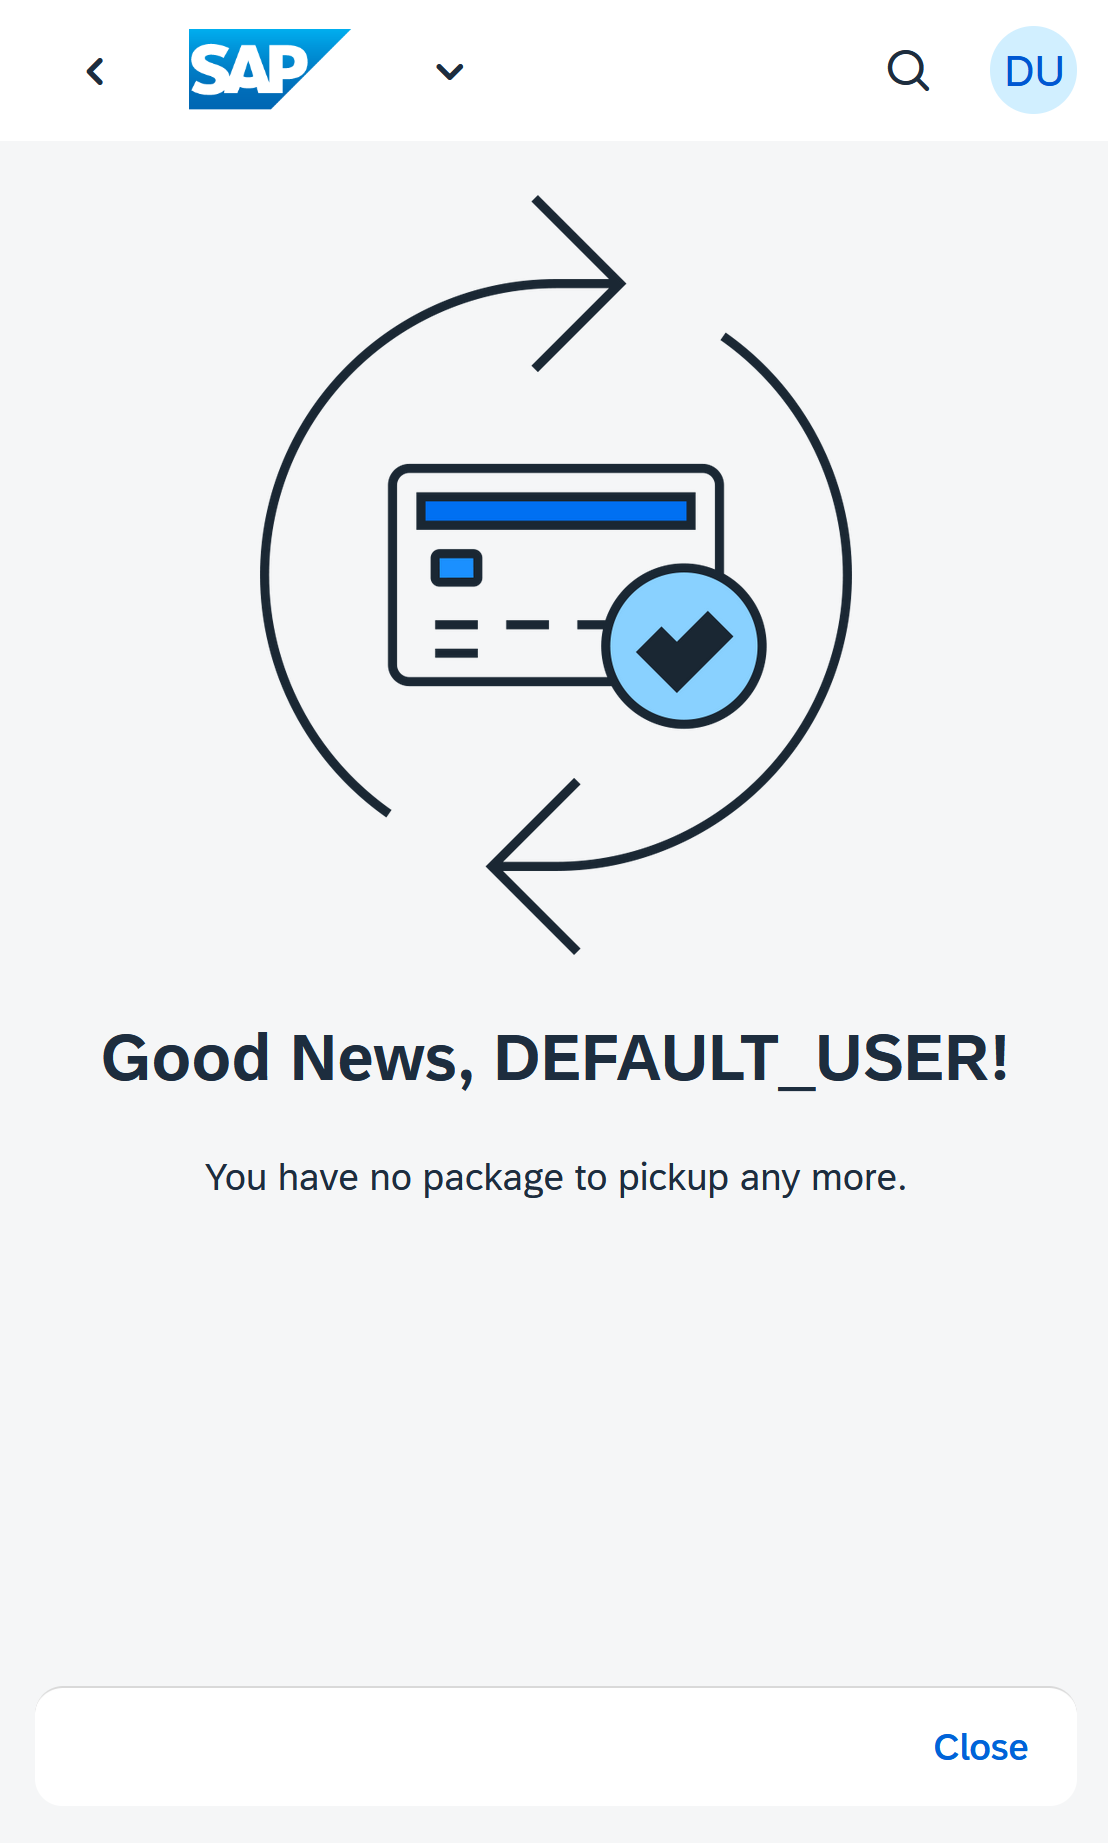
\includegraphics[width=0.45\linewidth]{images/user_doc/pickup/DoneScreenNoPackage.png}}
	\caption{Pickup Done Screen - Package Existence Guide}
	\label{fig:PickupDoneScreen-1}
\end{figure}

\pagebreak

\section{Receptionist}
\label{sec:UdocReceptionist}

As a logged in \textbf{Receptionist} (See \autoref{sec:GeneralRequisite} for all possible roles), one is granted to access the two applications under the \textbf{Parcel Handling} section, namely \textbf{Register Packages} (\autoref{subsec:rp}) and \textbf{Manage Packages} (\autoref{subsec:mp}). One can quick jump to the section by left clicking the "Parcel Handling" tab. One can enter the application by left click the tiles. (\autoref{fig:PHApplications})

\begin{figure}[H]
	\centering
	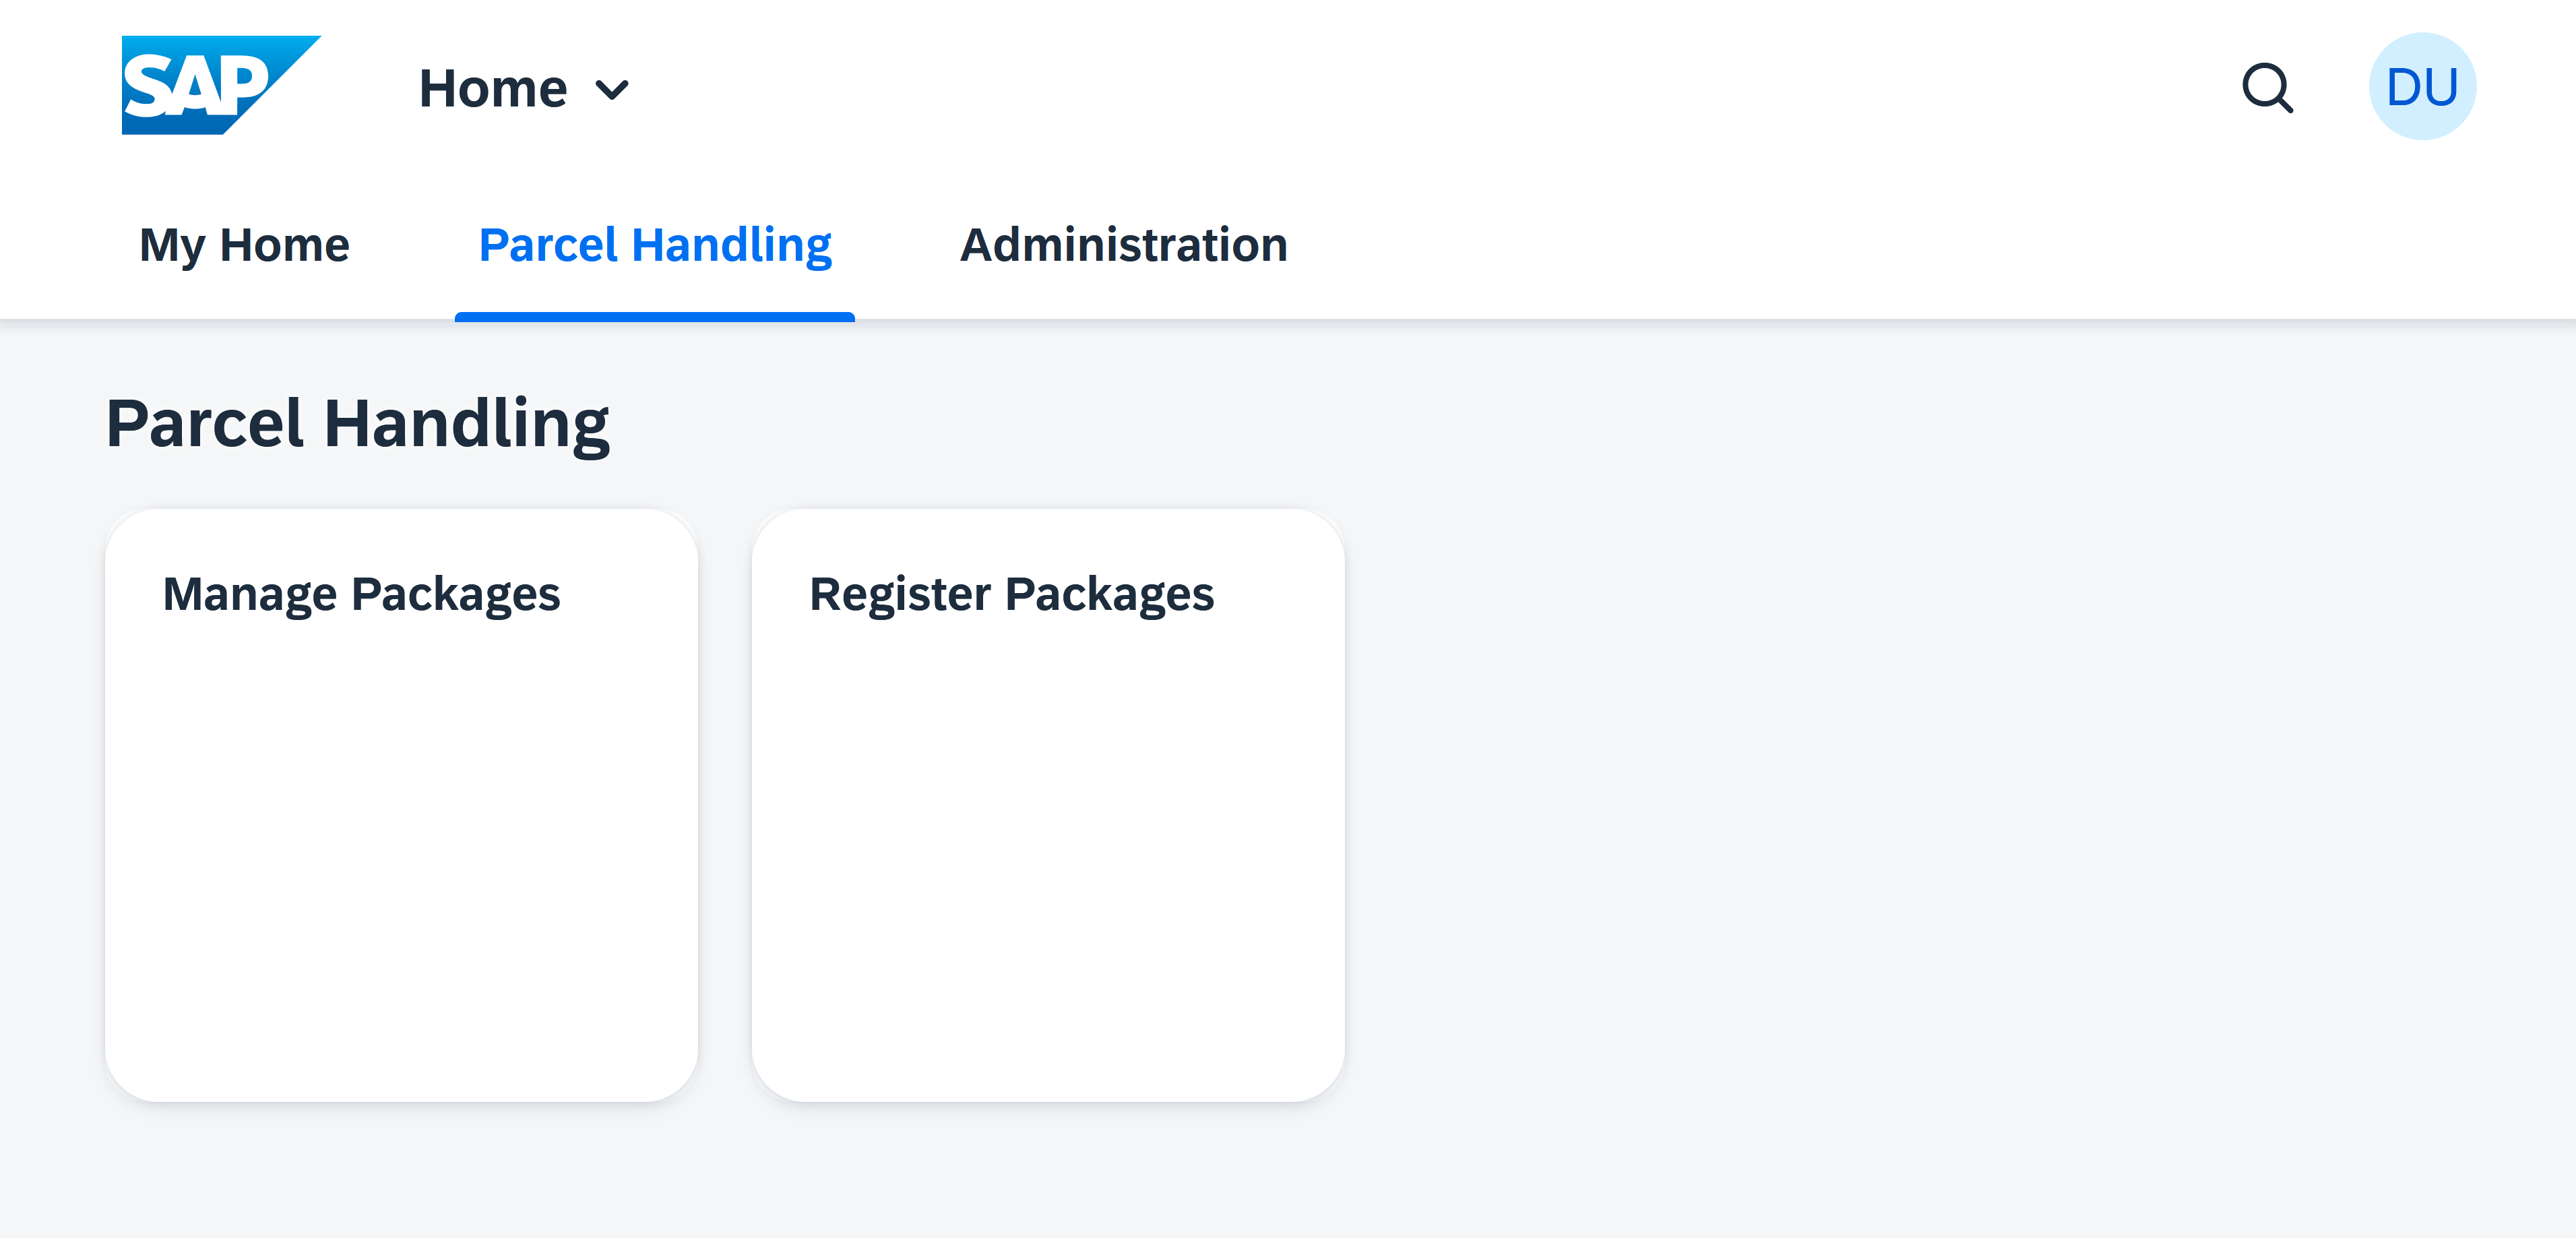
\includegraphics[width=1\linewidth]{images/user_doc/overviews/ParcelHandlingTab.png}
	\caption{Parcel Handling Applications}
	\label{fig:PHApplications}
\end{figure}


\subsection{Register Packages}
\label{subsec:rp}

When the delivery person arrived at the reception with the new parcels, the \textbf{Receptionist} shall use \textbf{Register Packages} application to register the newly arrived parcels into the system. (See \autoref{sec:UdocReceptionist} for all receptionist related applications) After the registration, \textbf{Receptionist} will be automatically redirected to  \textbf{Manage Packages}.
The summarized main actions the \textbf{Receptionist} can take within the application are listed here:

\begin{compactenum}
	\item Register a newly arrived package.
    \item Register multiple newly arrived packages.
    \item Discard current registration.
\end{compactenum}

\subsubsection{Data Entry}

As an \textbf{Receptionist}, by clicking at the \textbf{Register Packages} application tile, is redirected to the "Registration Form" (\autoref{fig:RPOverview}), which is the main and only screen of this application. At this point, \textbf{Recipient}, \textbf{Type}, \textbf{} and optionally \textbf{Comment} of the package are required by the form. (\autoref{fig:RPformEntry})

\begin{figure}[H]
	\centering
	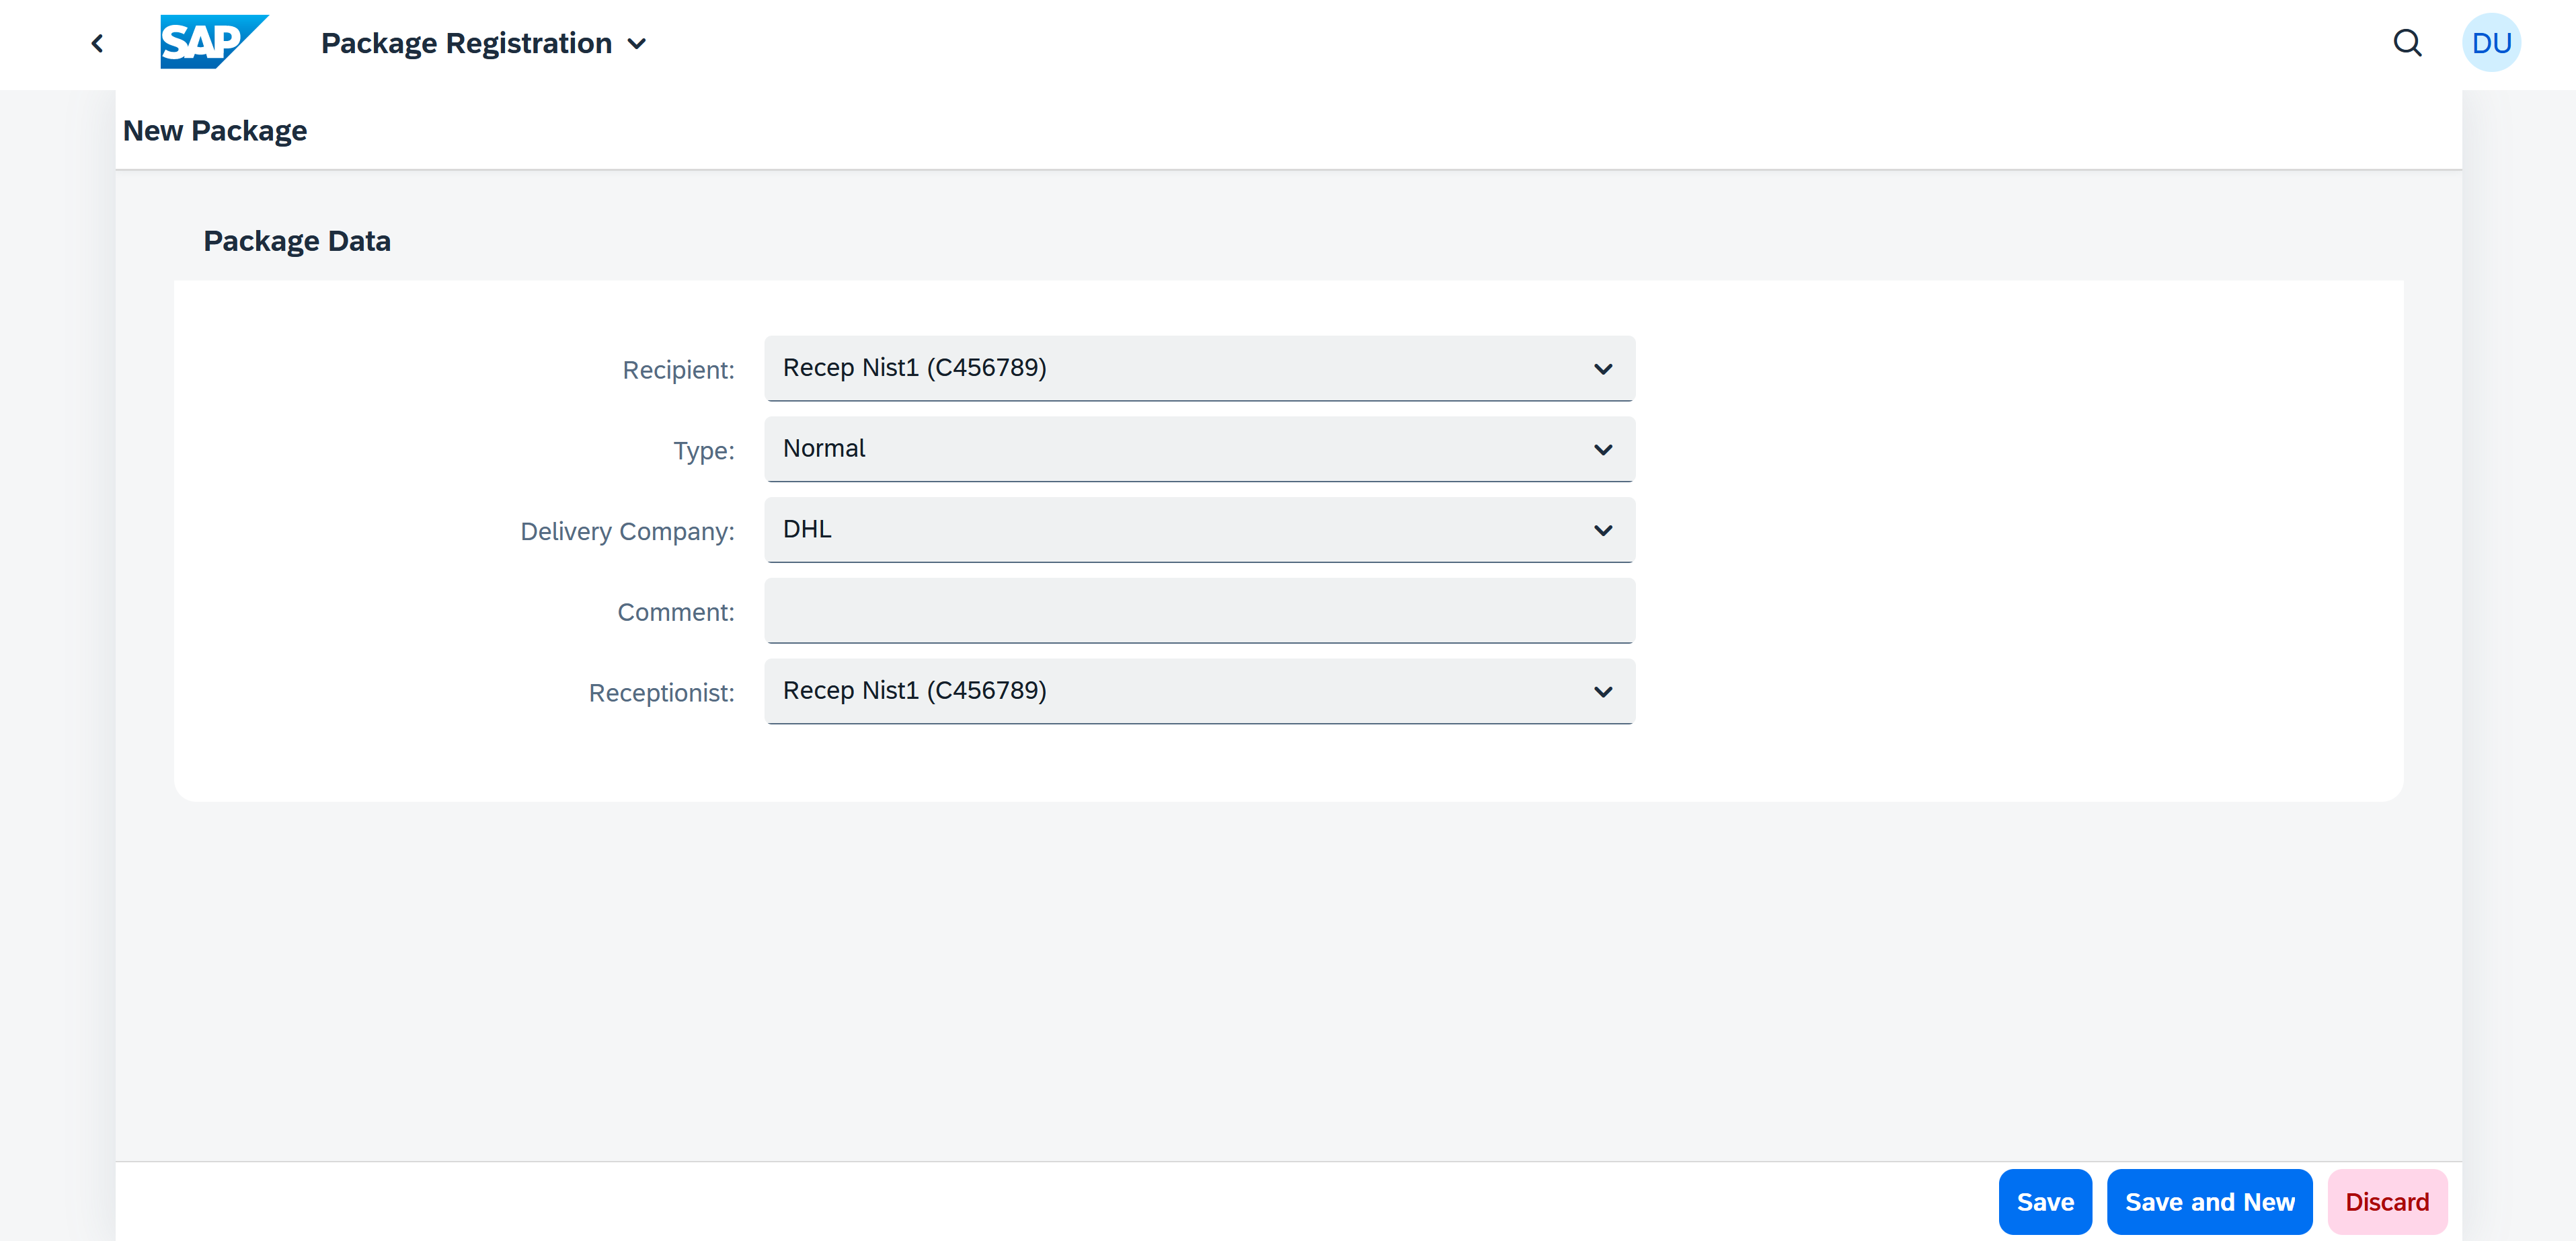
\includegraphics[width=1\linewidth]{images/user_doc/registration/overview.png}
	\caption{Register Packages Form - Overview}
	\label{fig:RPOverview}
\end{figure}


\begin{figure}[H]
	\centering
	\subcaptionbox{Step 1: Choose Recipient}{
		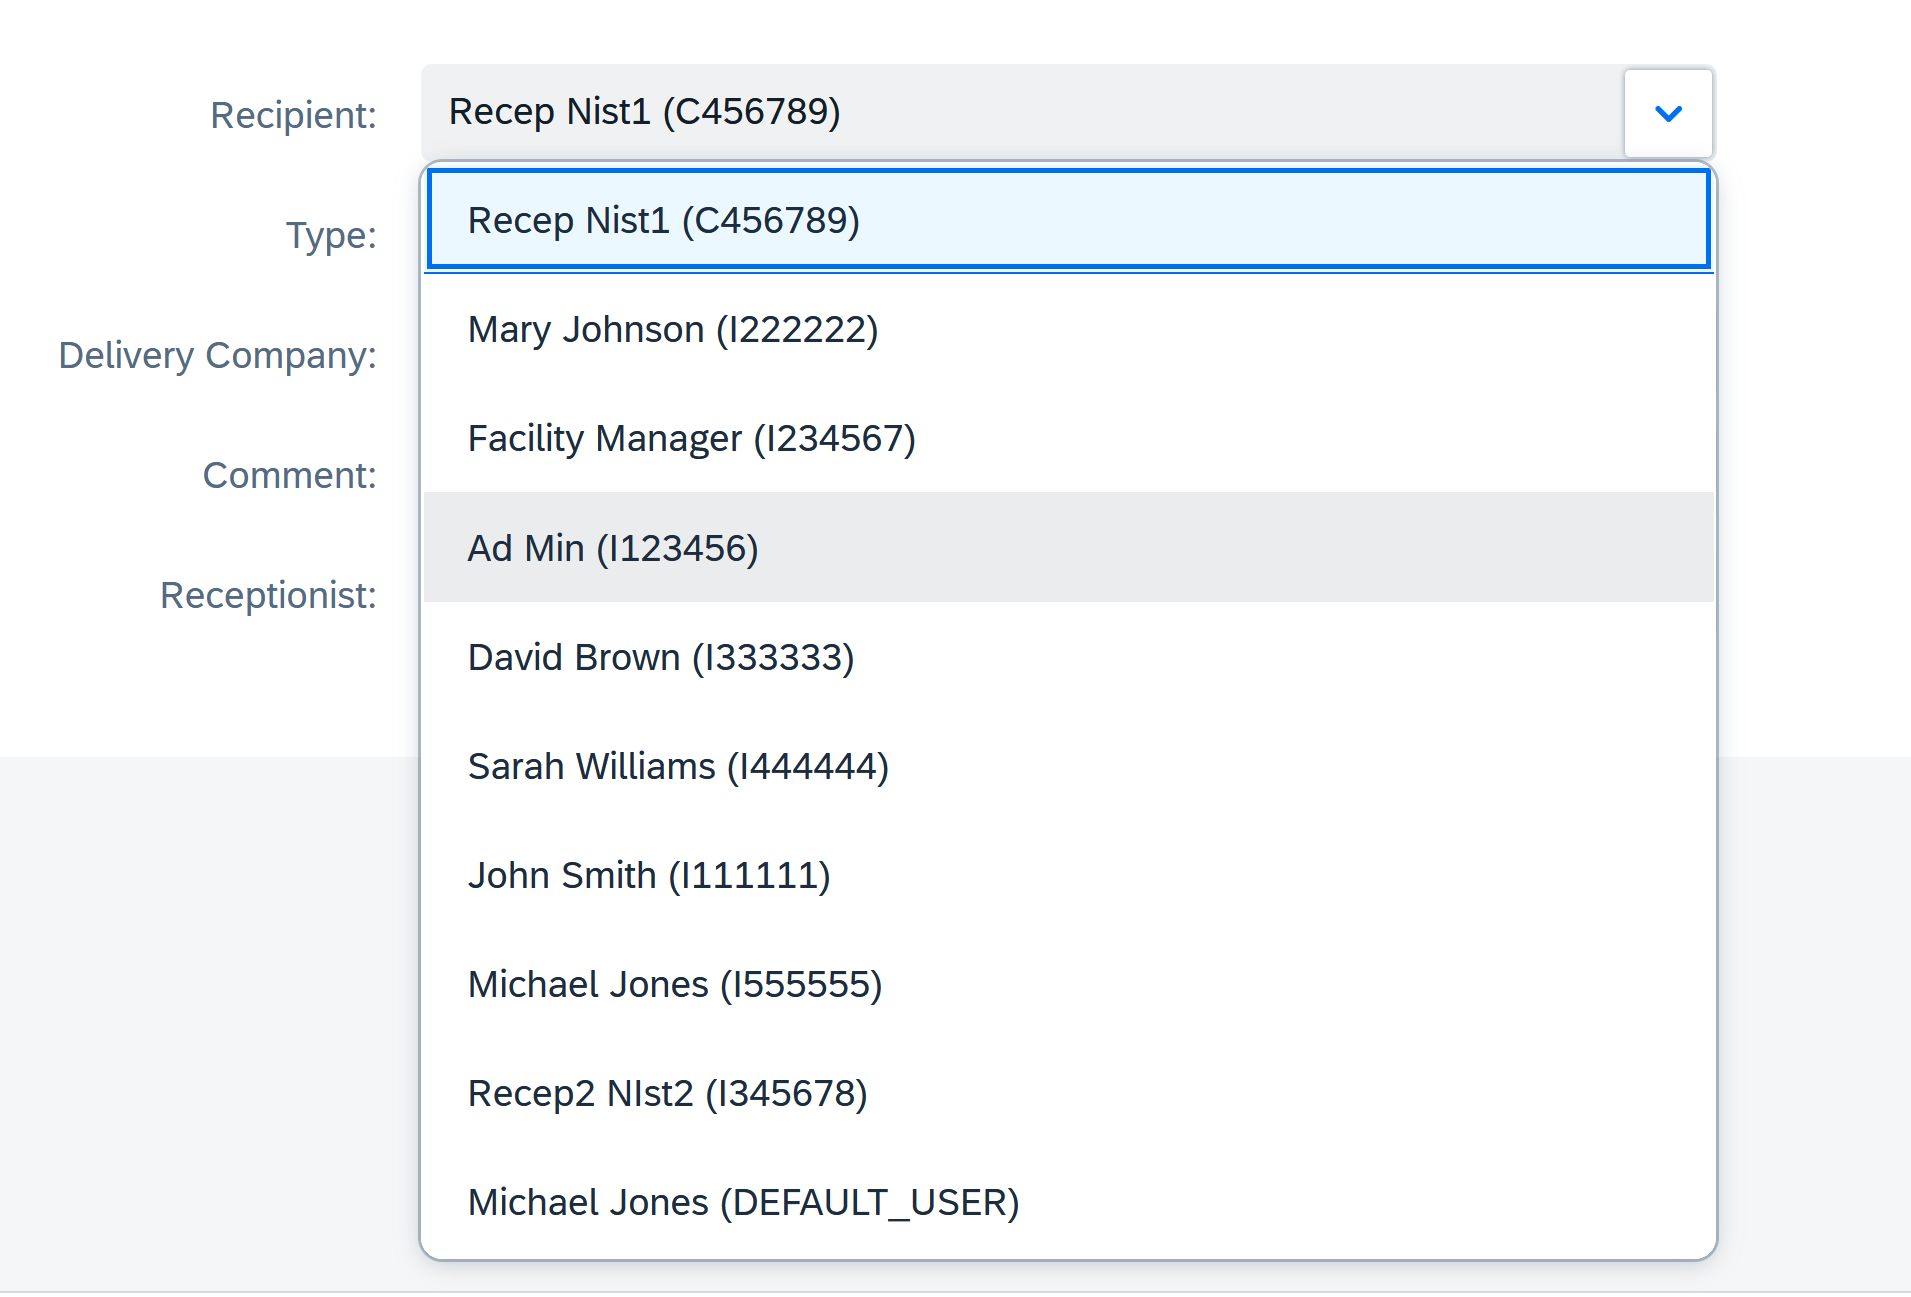
\includegraphics[width=0.45\linewidth]{images/user_doc/registration/entry1.png}}
   \hspace{5pt}
    \subcaptionbox{Step 2: Choose Package Type}{
		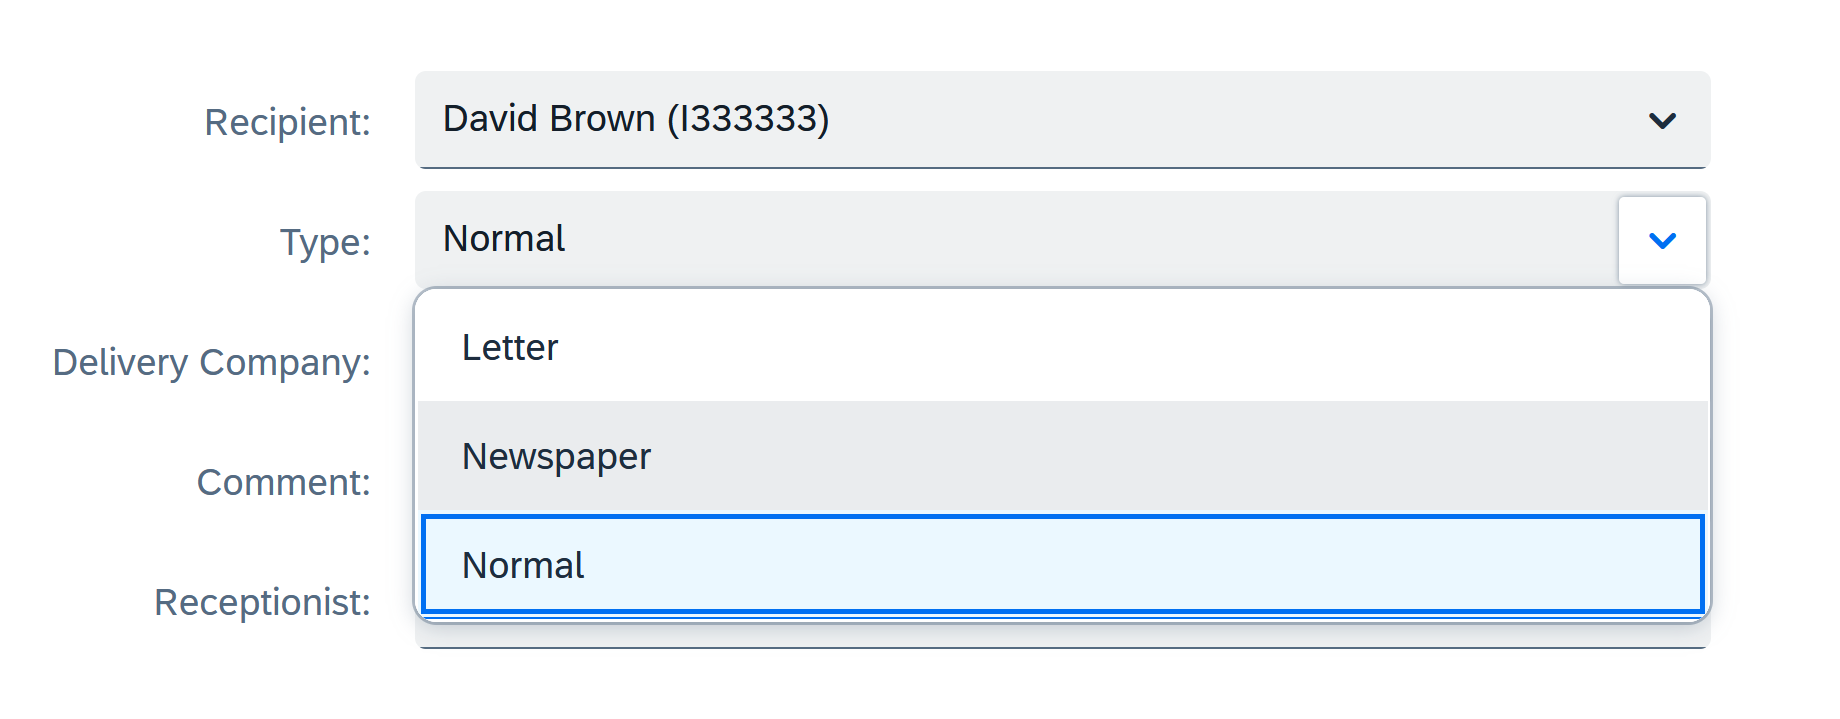
\includegraphics[width=0.45\linewidth]{images/user_doc/registration/entry2.png}}
  
	\subcaptionbox{Step 3: Choose Delivery Company}{
		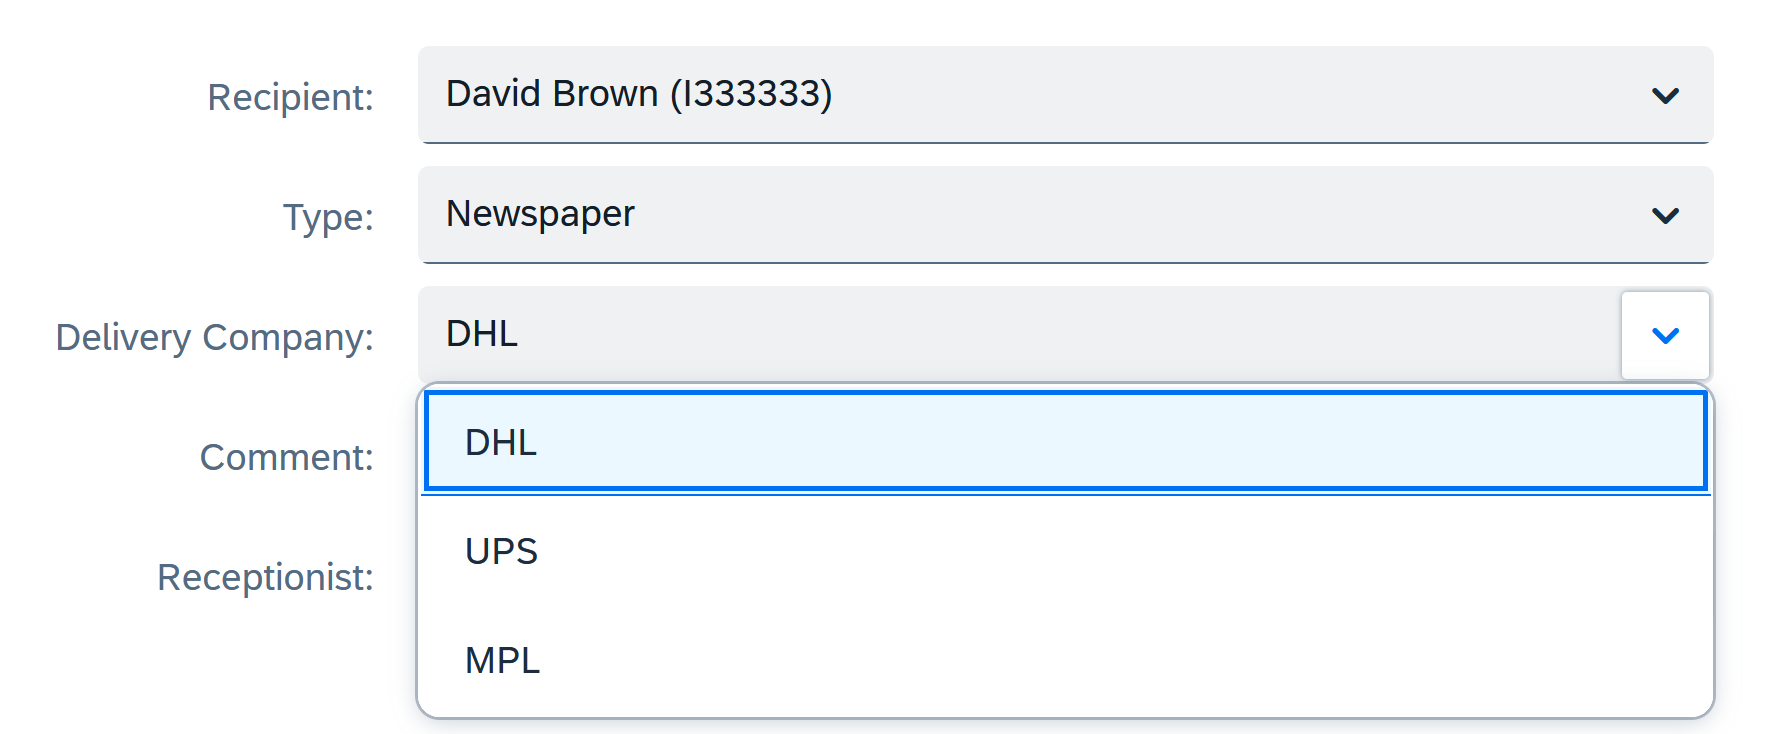
\includegraphics[width=0.45\linewidth]{images/user_doc/registration/entry3.png}}
    \hspace{5pt}
    \subcaptionbox{Step 4: Input any Comment if Needed}{
		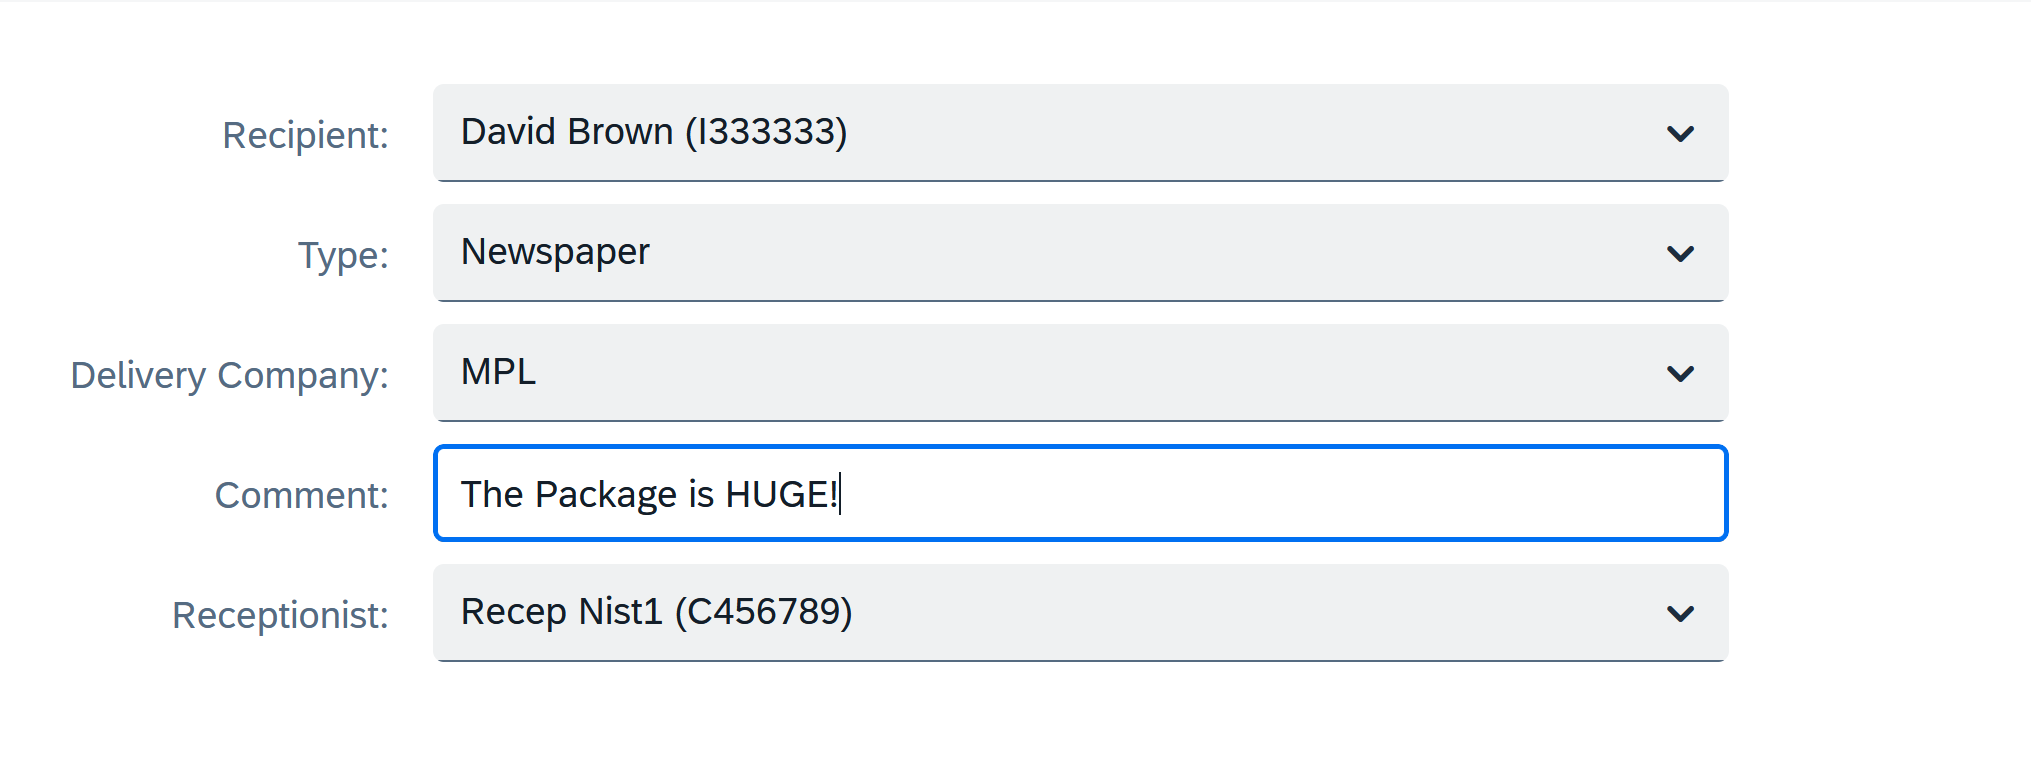
\includegraphics[width=0.45\linewidth]{images/user_doc/registration/entry4.png}}

    	\subcaptionbox{Step 3: Choose Responsible Receptionist}{
		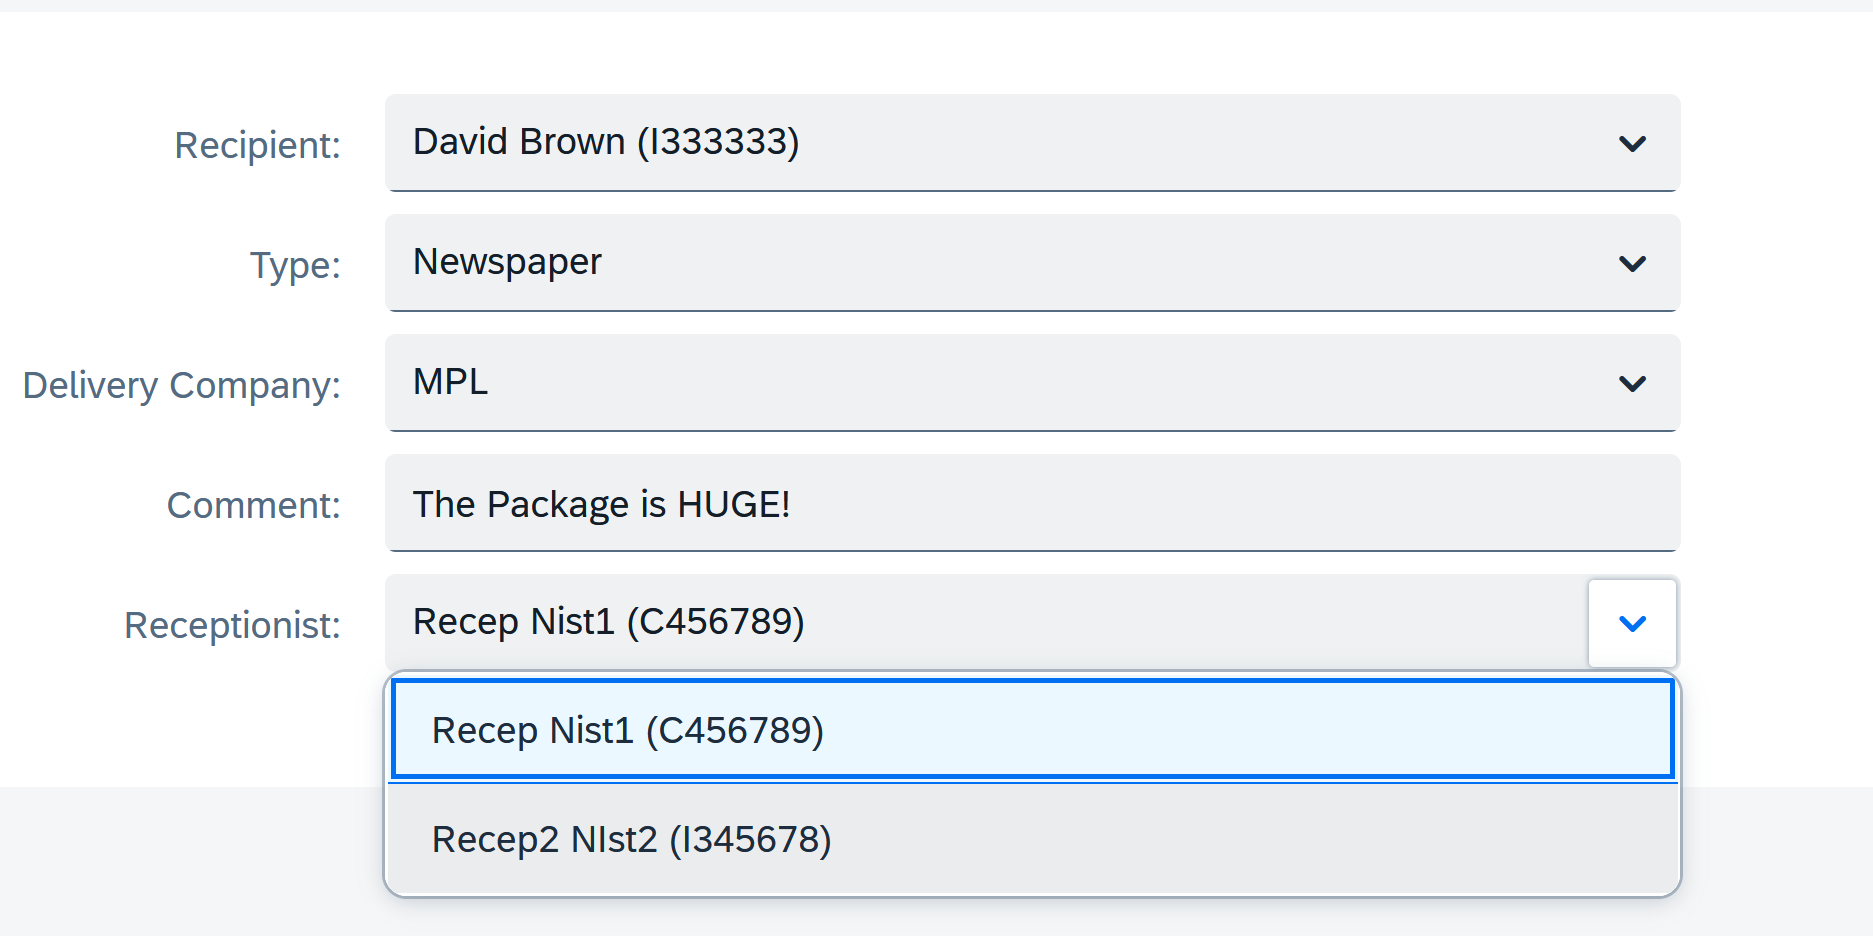
\includegraphics[width=0.45\linewidth]{images/user_doc/registration/entry5.png}}
  
    \caption{Register Packages Form - Form Entry Guide}
	\label{fig:RPformEntry}
\end{figure}

\subsubsection{Data Submitting}

When \textbf{Receptionist} finished entering the form and click the "Save" button, the entered package details are submitted, a package with \textit{new} status is created in the system, a success message toast appears and \textbf{Receptionist} is then navigated automatically to the \textbf{Manage Package} application. (\autoref{fig:RPsaveOp})

When \textbf{Receptionist} finished entering the form and click the "Save and New" button, the entered package details are submitted, a package with \textit{new} status is created in the system, a success message toast appears and the form is reset to default state. \textbf{Receptionist} may then start to register another package. (\autoref{fig:RPsaveNewOp})

When \textbf{Receptionist} finished entering the form and click the "Discard" button, the form is reset to default state and \textbf{Receptionist} is navigated back to the launch pad. (\autoref{fig:RPdiscardOp})

\begin{figure}[H]
	\centering
    \begin{subfigure}{1\linewidth}
        \centering
        \subcaptionbox {Success Toast}{
            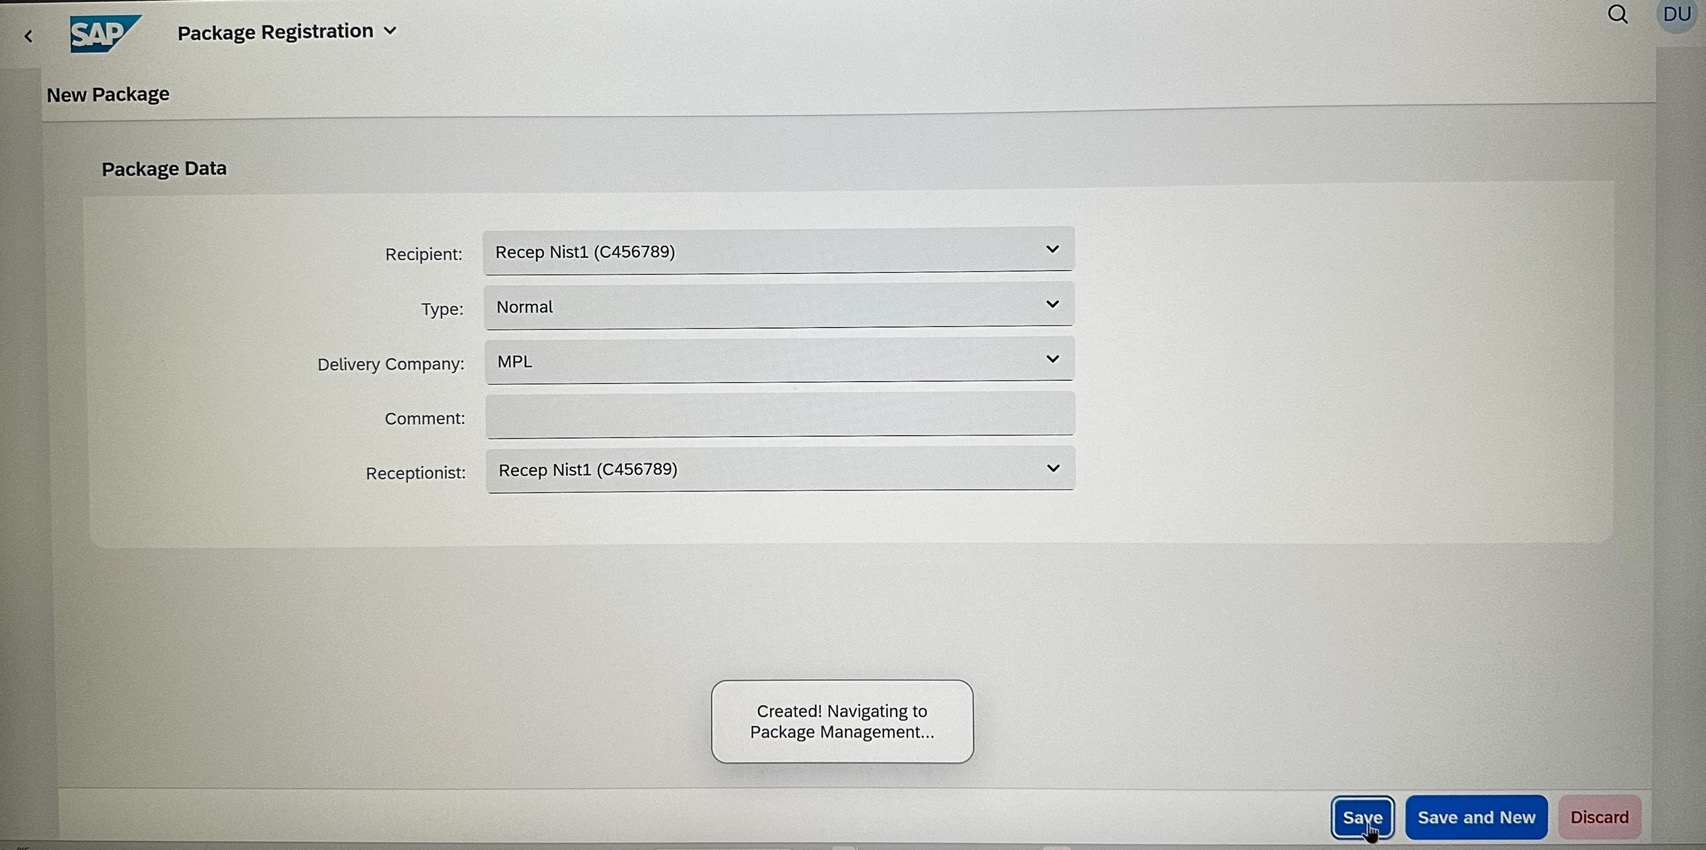
\includegraphics[width=0.45\linewidth]{images/user_doc/registration/SaveToast.jpg}
        }
        \vspace{5pt}
        \subcaptionbox {Target Navigation - Manage Package}{
            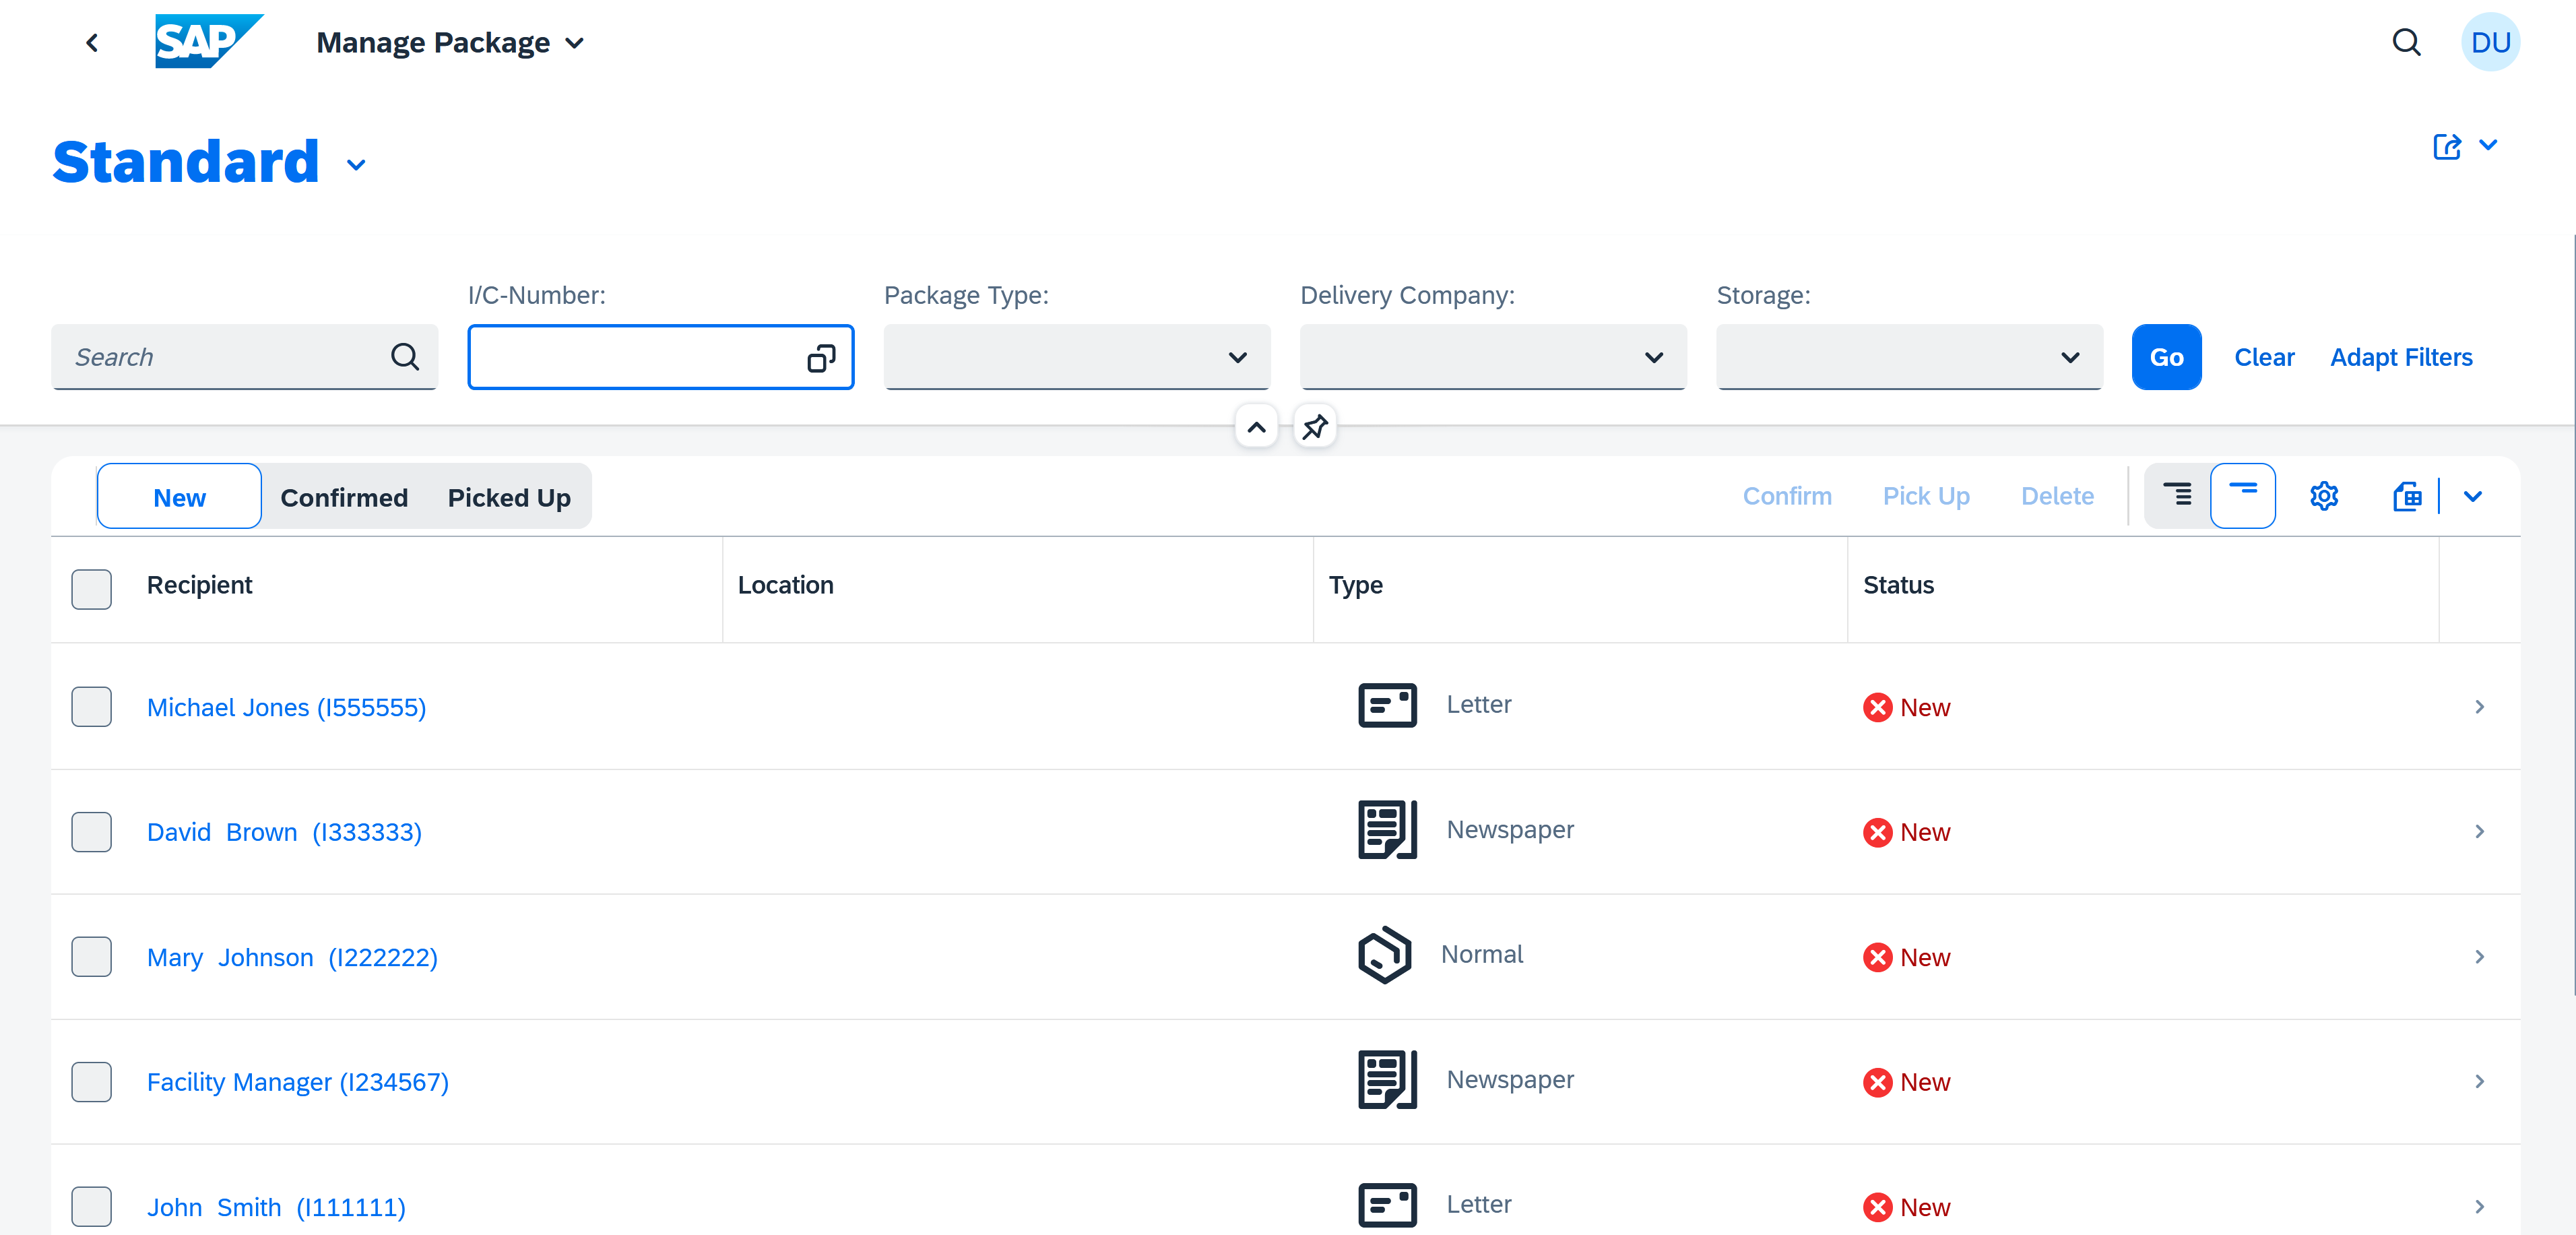
\includegraphics[width=0.45\linewidth]{images/user_doc/registration/target.png}
        }
        \caption{Option 1: Save}
    \end{subfigure}%
    \caption{Register Packages Form - Option 1: Save}
    \label{fig:RPsaveOp}
\end{figure}

\begin{figure}[H]
	\centering
    \begin{subfigure}{1\linewidth}
        \centering
        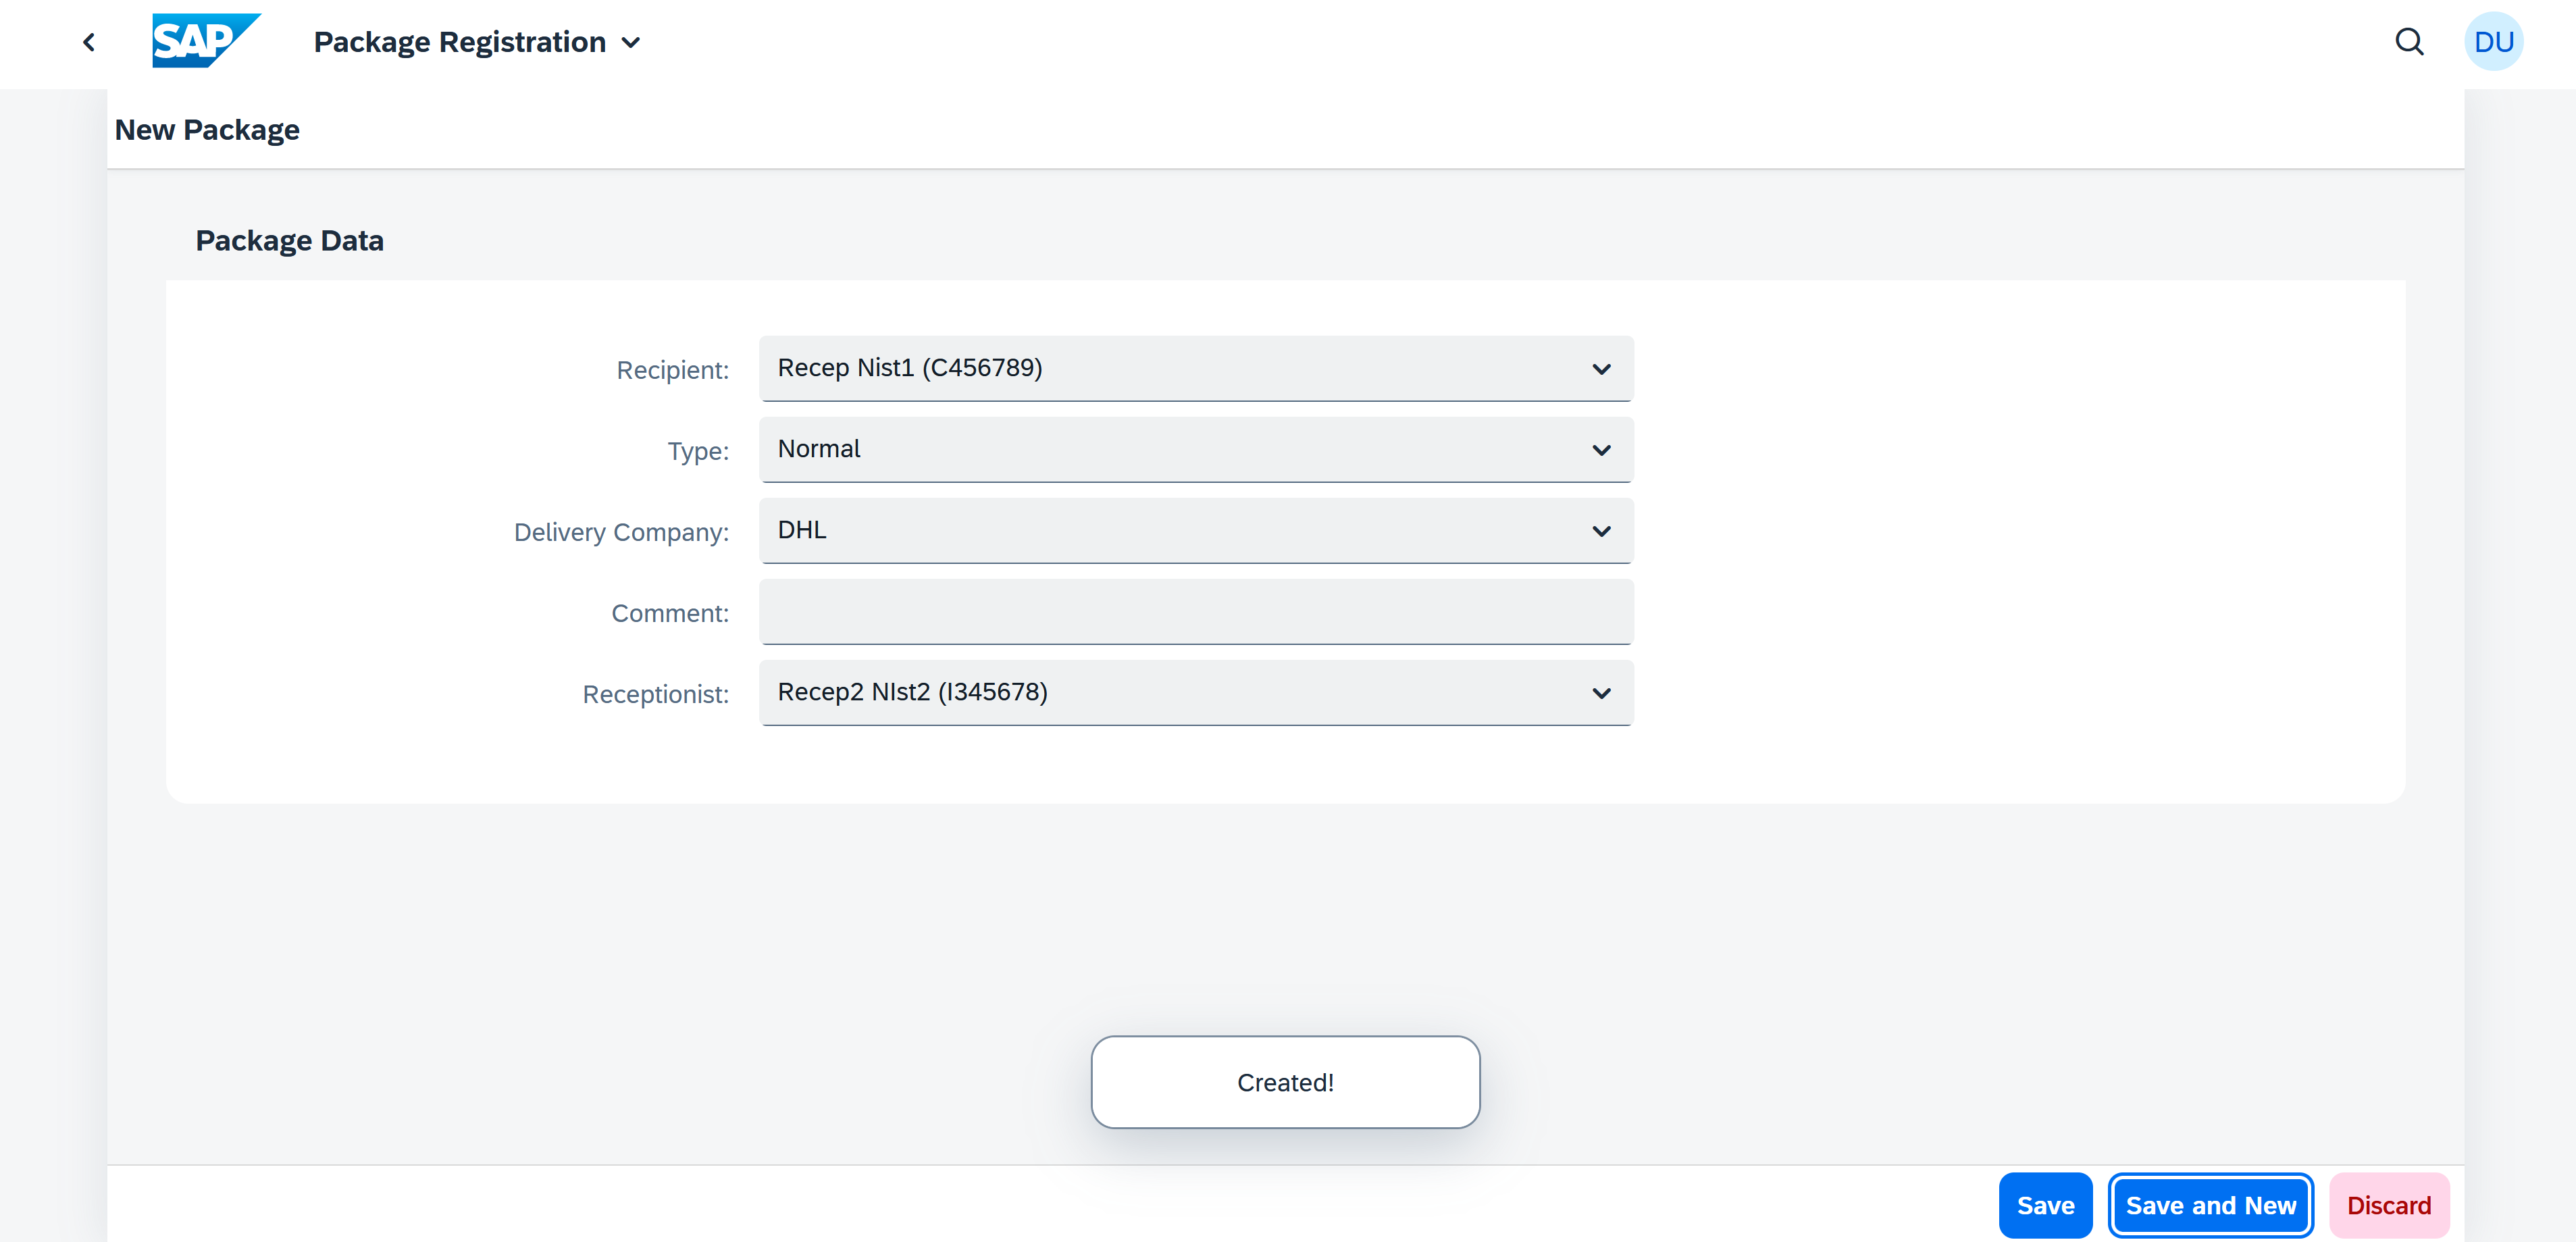
\includegraphics[width=1\linewidth]{images/user_doc/registration/saveAndNewToast.png}
    \end{subfigure}
    \caption{Register Packages Form - Option 2: Save and New}
    \label{fig:RPsaveNewOp}
\end{figure}

\begin{figure}[H]
	\centering
    \begin{subfigure}{1\linewidth}
        \centering
        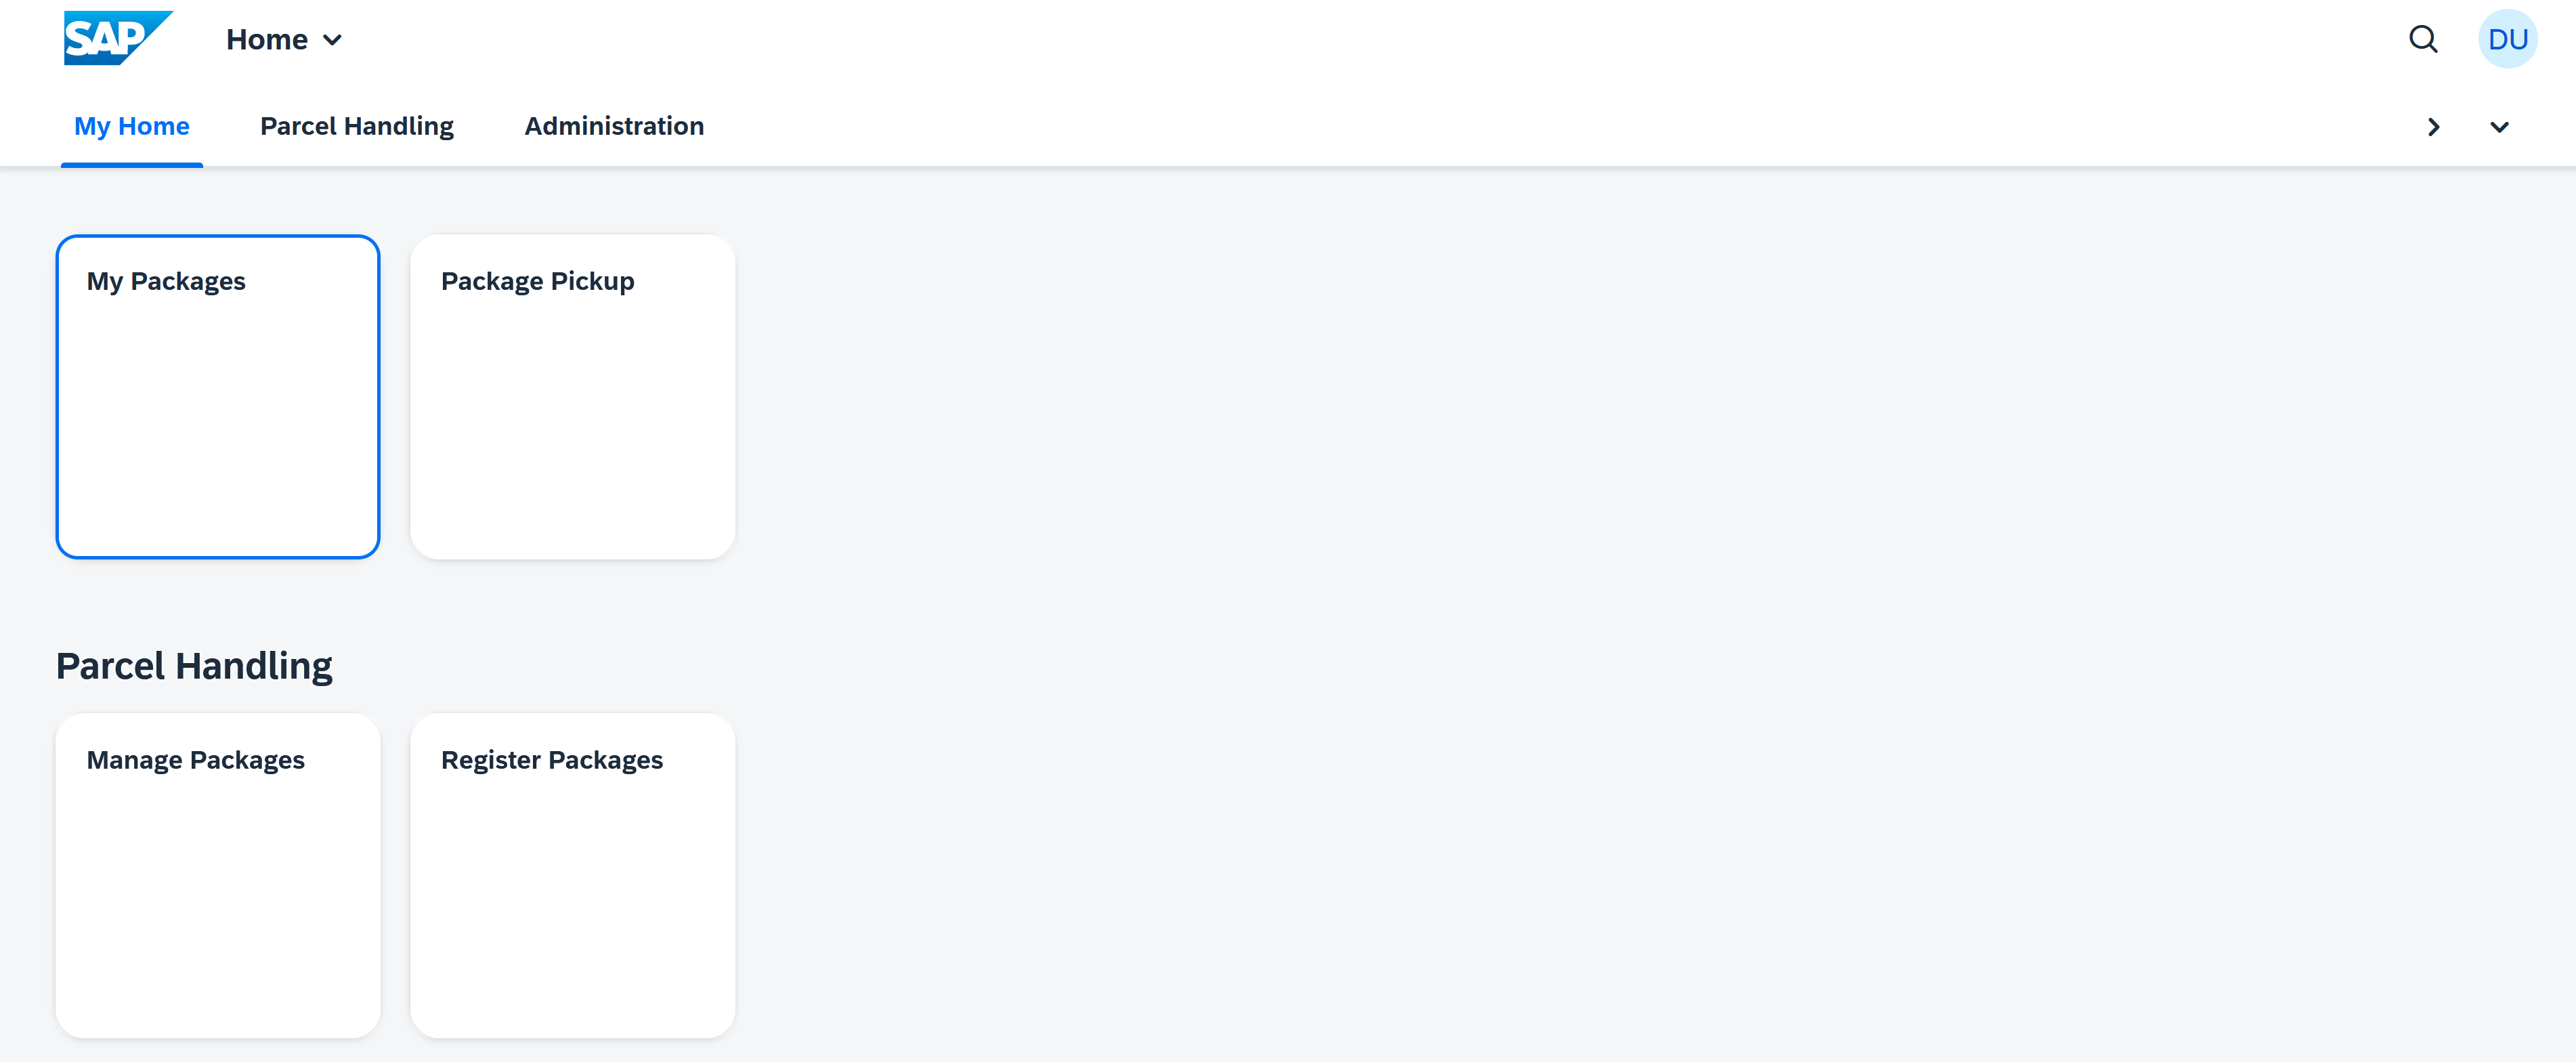
\includegraphics[width=1\linewidth]{images/user_doc/registration/discardTarget.png}
    \end{subfigure}
    \caption{Register Packages Form - Option 3: Discard}
    \label{fig:RPdiscardOp}
\end{figure}

\subsection{Manage Packages}                     
\label{subsec:mp}

The \textbf{Manage Packages} application is designed for \textbf{Receptionist} (See \autoref{sec:UdocReceptionist} for all receptionist related applications) to edit, confirm, pickup, check the existing packages in the system. The summarized main actions a \textbf{Receptionist} can take are listed here:

\begin{compactenum}
	\item Browse the existing packages.
        \begin{compactenum}
            \item Filtering possibility.
            \item Quick variant switch based on package status.
            \item Report List of packages info with selection capability.
            \item Detail page for single packages.
        \end{compactenum}
    \item Confirm package(s) which status is new.
    \item Pickup a package (single at a time) which status is confirmed. (As a backup manuvor in case the employee cannot access to mobile devices.
    \item Delete package(s) which status is new or confirmed.
    \item Edit package(s)' recipient, type, delivery company, and comment.
\end{compactenum}

\bigskip
Further explanation and restrictions of these operations are detailed in the coming sections.

\begin{figure}[H]
	\centering
	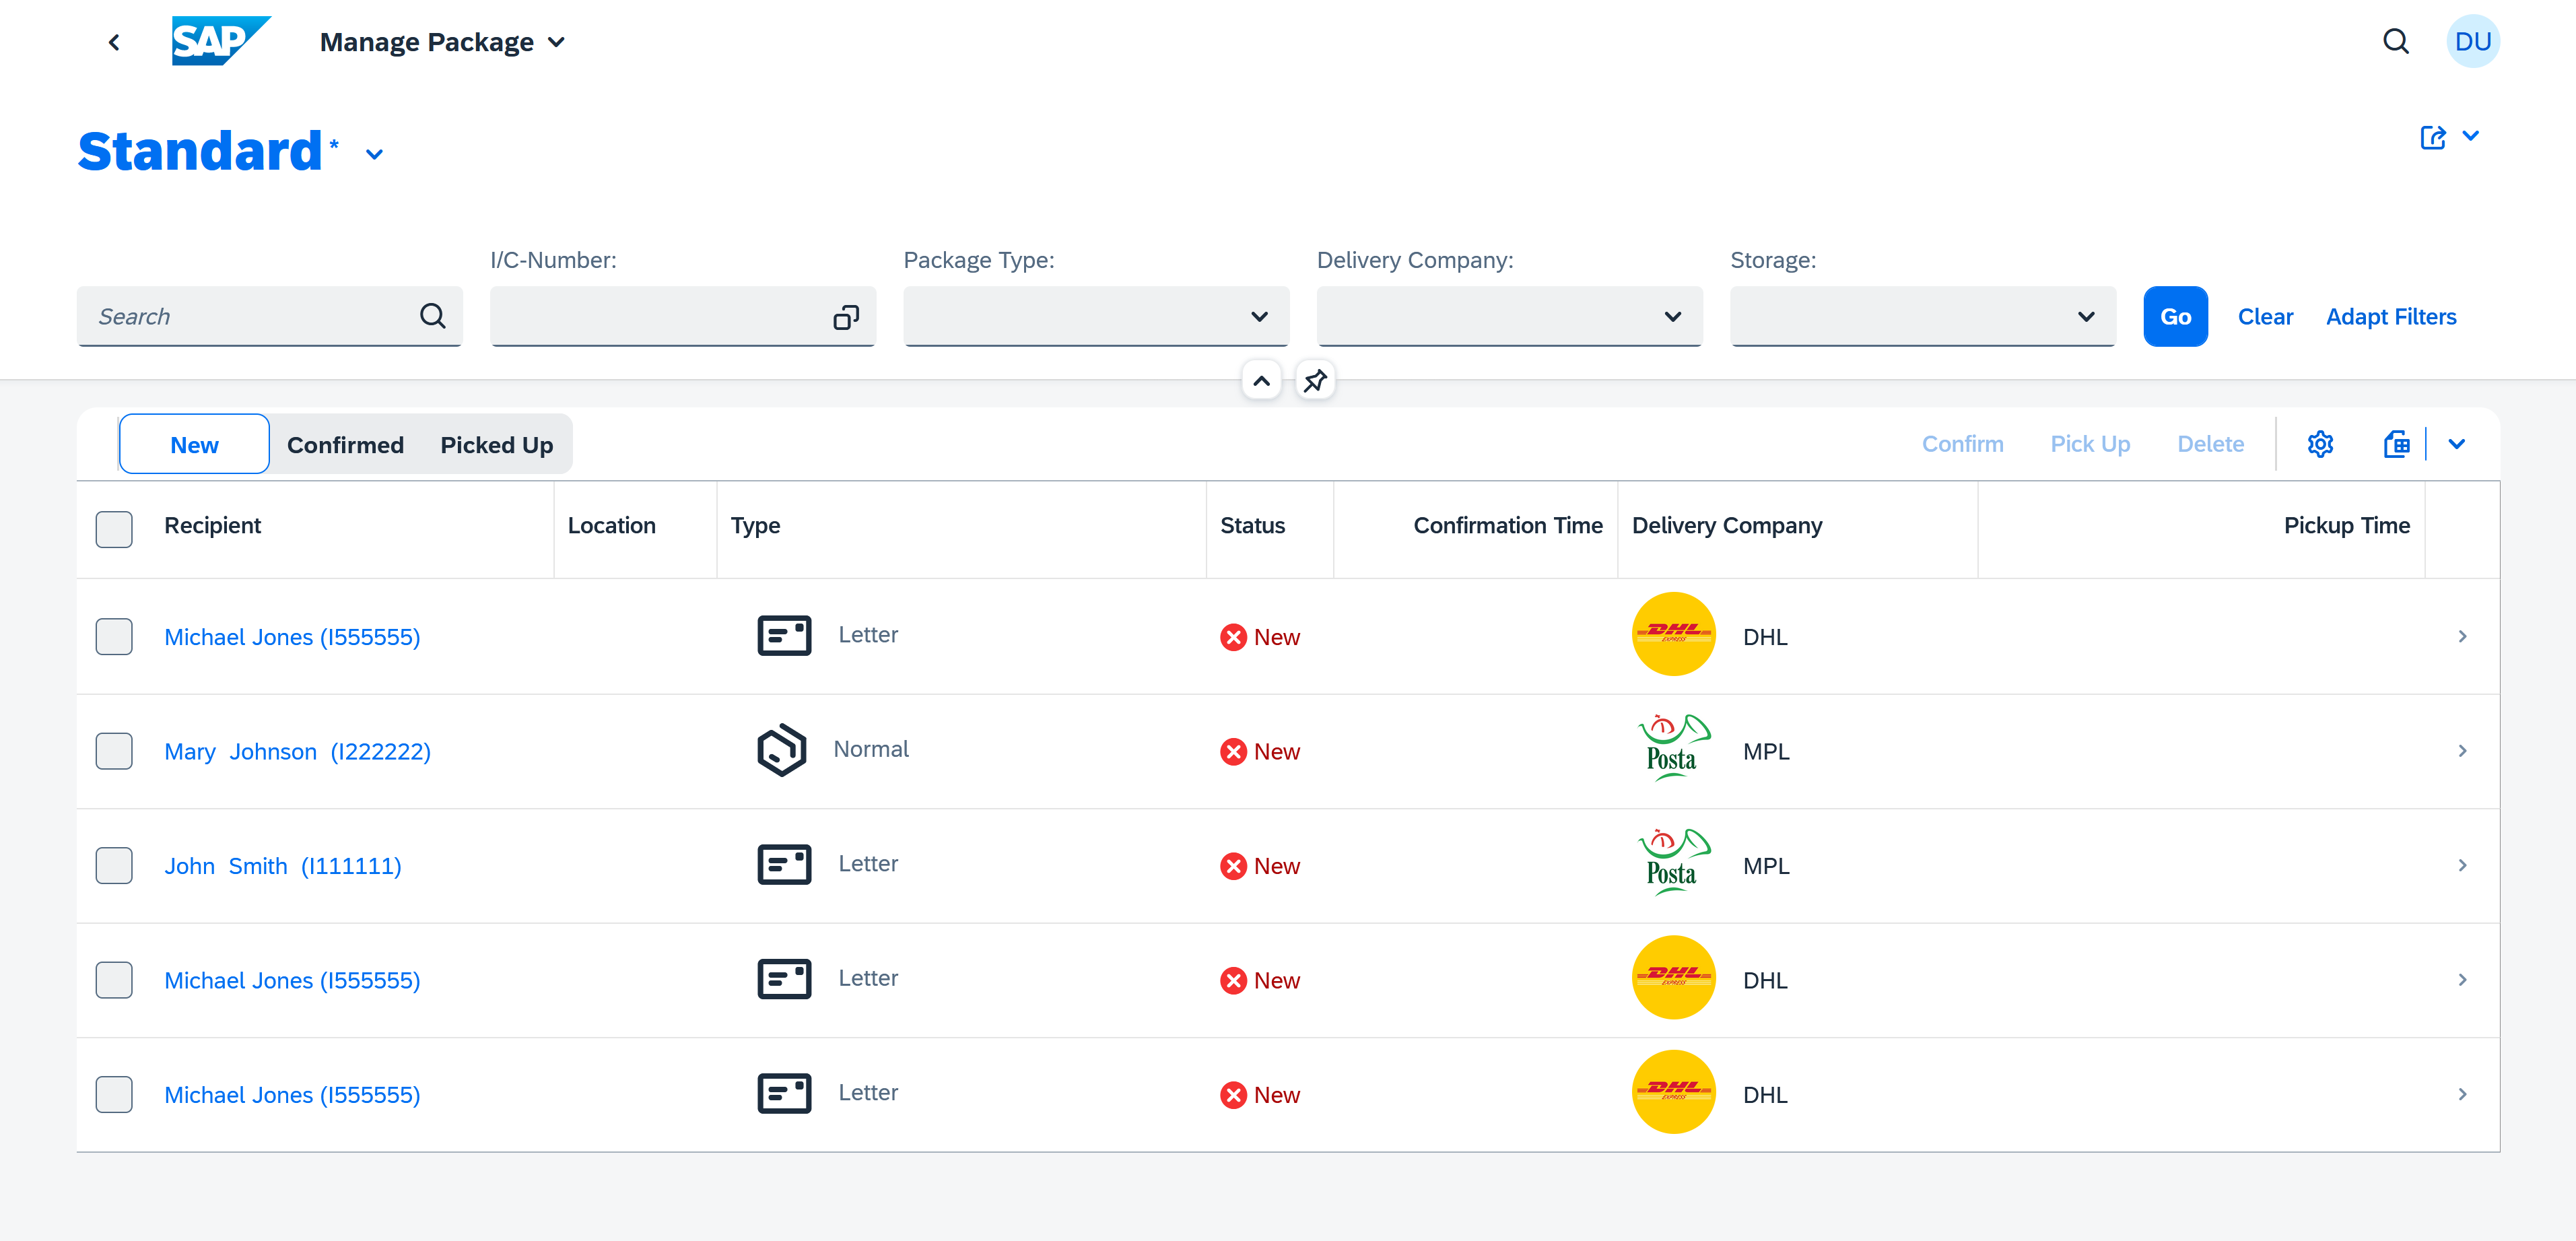
\includegraphics[height=200pt]{images/user_doc/managePack/ReportScreen/browse/Overview.png}
	\caption{Manage Packages Report Screen - Overview}
	\label{fig:MPReportOverview}
\end{figure}


\subsubsection{Browse Packages}
As an \textbf{Receptionist}, after clicking at the application tile, is redirected to the "Report Screen", which is the main screen of this application (\autoref{fig:MPReportOverview}). 
The upper part displays the search bar and the possible filters (\autoref{fig:MPFIlterBar}). 
In case the need of free text search of any possible content of the column, one can use the \textbf{"Search Bar"}. (\autoref{fig:MPSearchBar}) The search supports in-completed keywords and is case insensitive. One can also use the predefined filters, where value helps and entry helps are provided.
The default predefined filters are: \textbf{I/C-Number} (free text SAP ID input, \autoref{fig:MPIDFIlter}), \textbf{Type} (drop down of all available types), \textbf{Delivery Company} (drop down of all available companies) and \textbf{Storage} (drop down of all available storage). 
For drop down filters, one can click at the small drop down arrow and select zero to many options (\autoref{fig:MPDefaultDropDown}). When adjusting the filtering values, the list view is temporarily locked. After adjusting the filtering values, one can run and review the filter result by clicking the "Go" Button. (\autoref{fig:MPAjustFilters})

\begin{figure}[H]
	\centering
	
\includegraphics[width=1\linewidth]{images/user_doc/managePack/ReportScreen/browse/FilterBar.png}
	\caption{Manage Packages Report Screen - Filter Bar}
	\label{fig:MPFIlterBar}
\end{figure}

\begin{figure}[H]
	\centering
	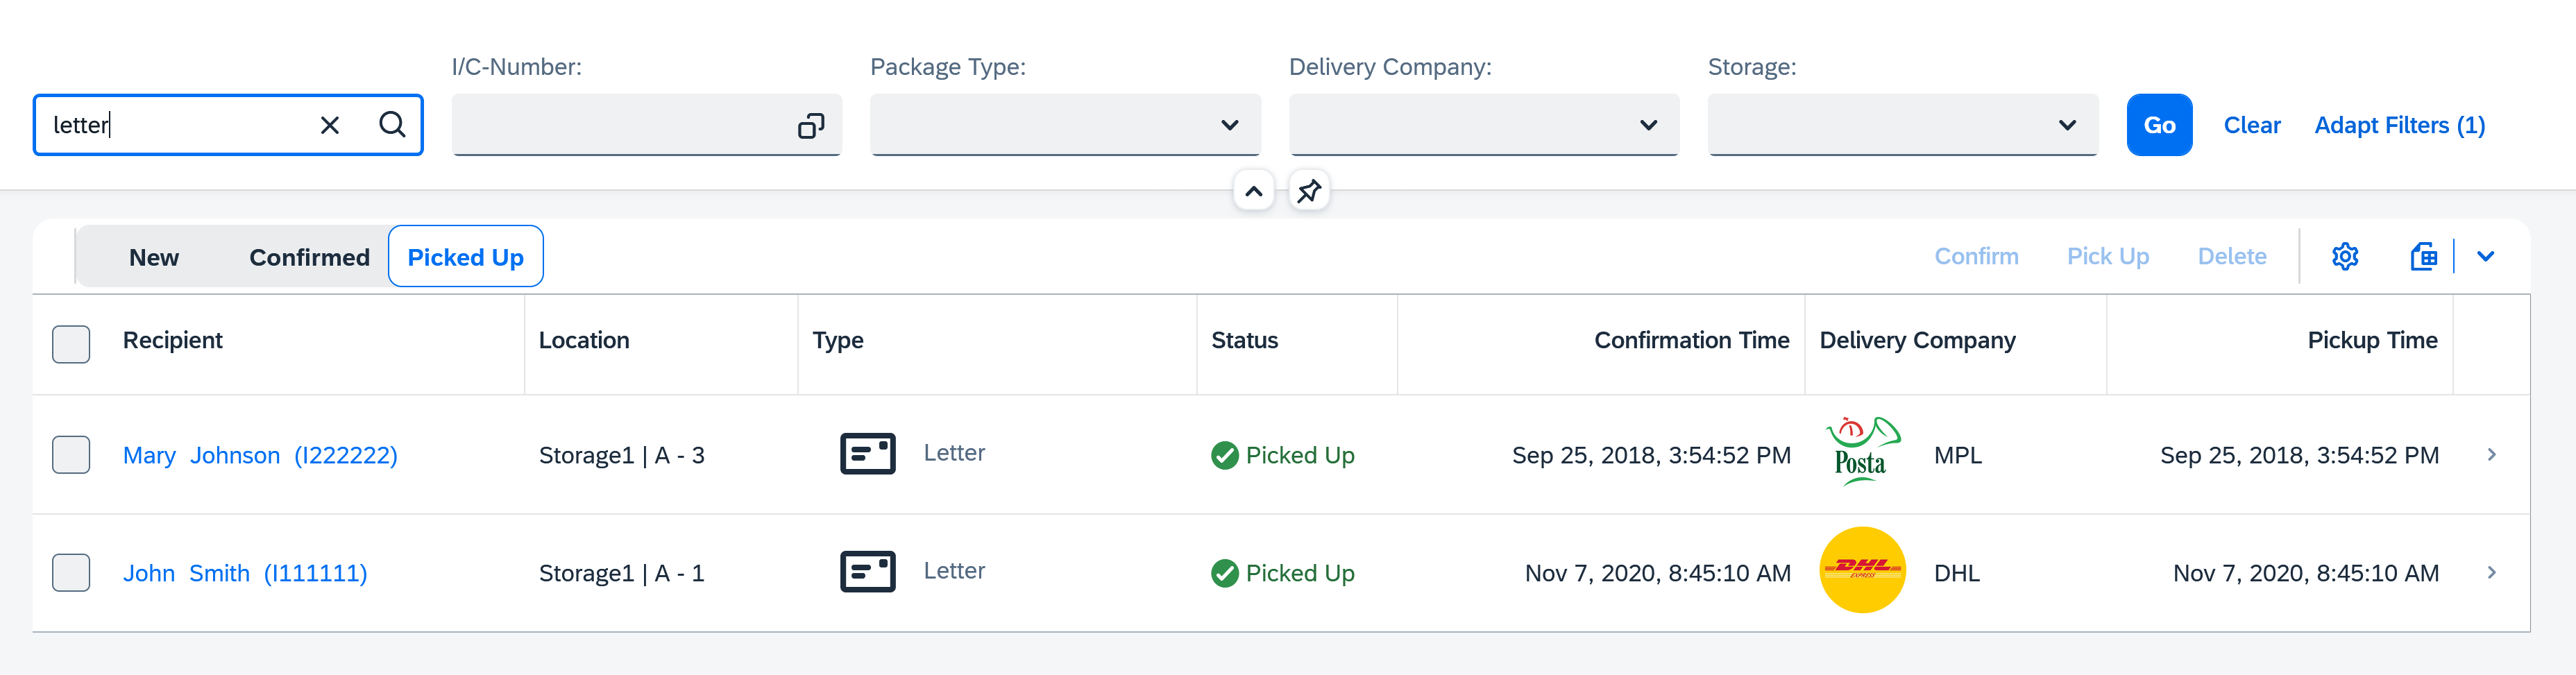
\includegraphics[width=1\linewidth]{images/user_doc/managePack/ReportScreen/browse/defaultSearchBarUsage.png}
	\caption{Manage Packages Report Screen - Filter Bar - Search Bar Usage Guide}
	\label{fig:MPSearchBar}
\end{figure}

\begin{figure}[H]
	\centering
	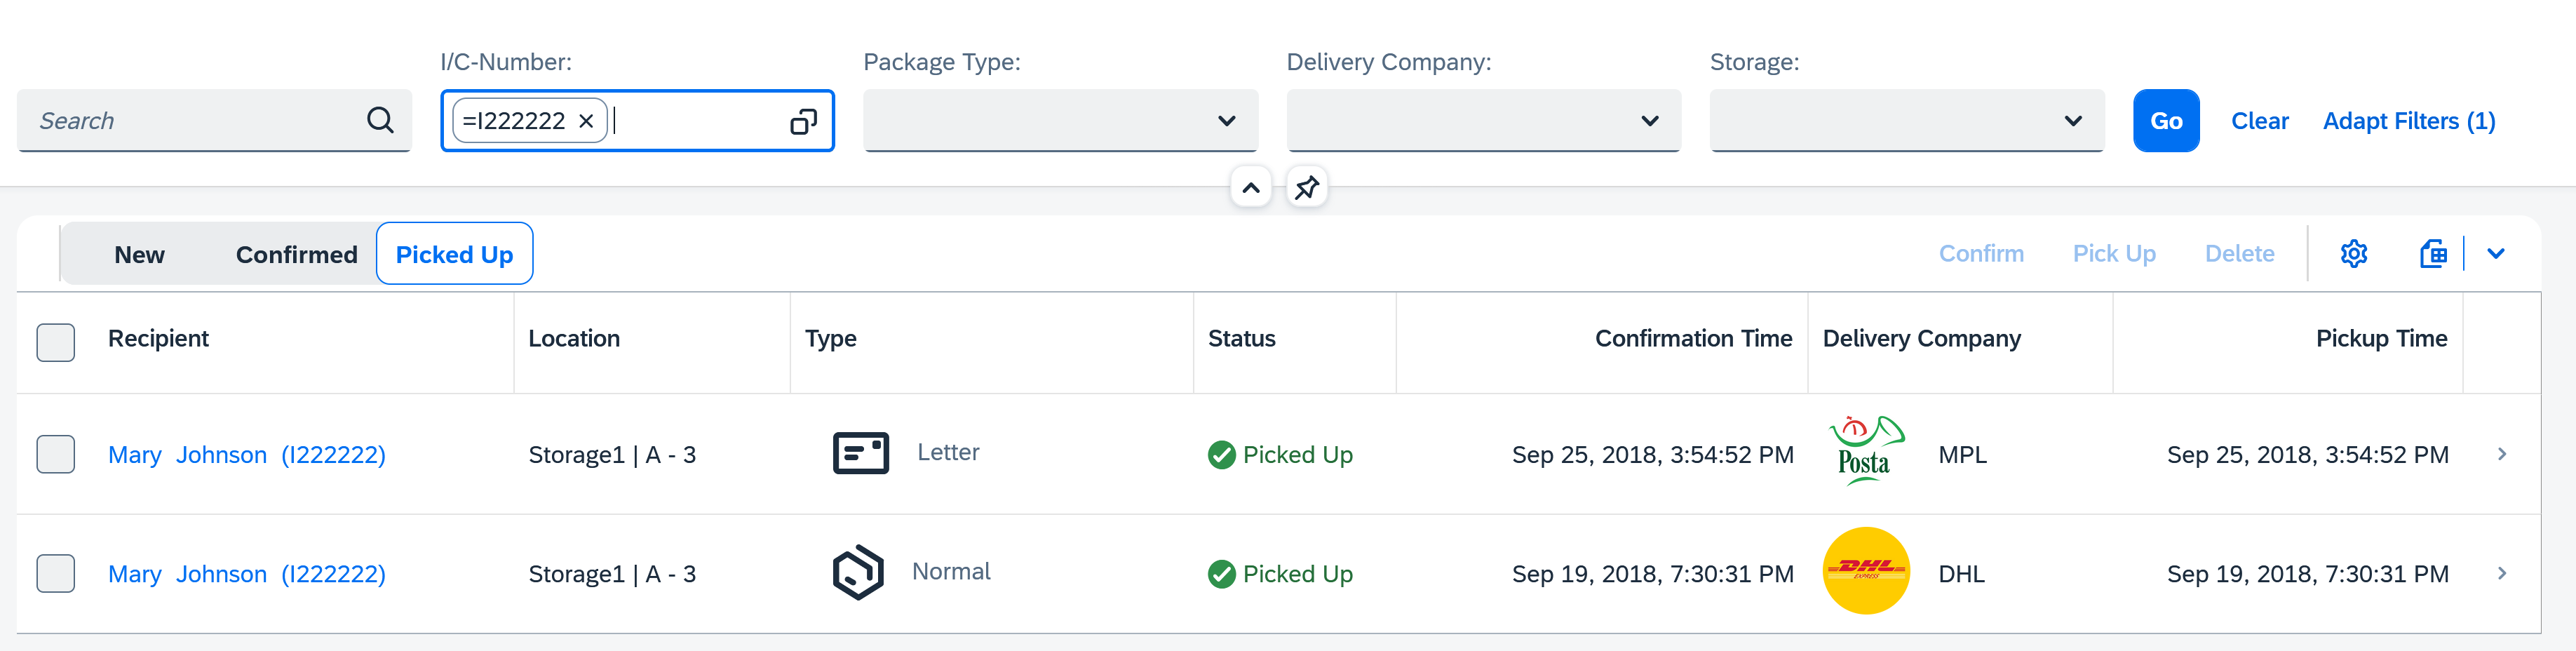
\includegraphics[width=1\linewidth]{images/user_doc/managePack/ReportScreen/browse/defaultFreeTextIdUsage.png}
	\caption{Manage Packages Report Screen - Filter Bar - ID Filter Usage Guide}
	\label{fig:MPIDFIlter}
\end{figure}

\begin{figure}[H]
	\centering
	\subcaptionbox{Type Filter}{
		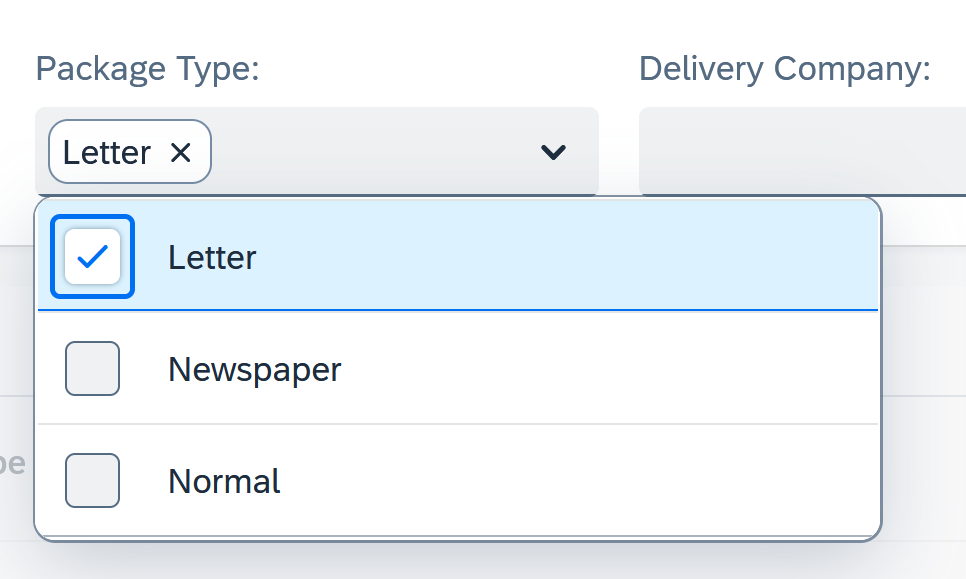
\includegraphics[width=0.45\linewidth]{images/user_doc/managePack/ReportScreen/browse/defaultType.png}}
	\hspace{5pt}
	\subcaptionbox{Company Filter}{
		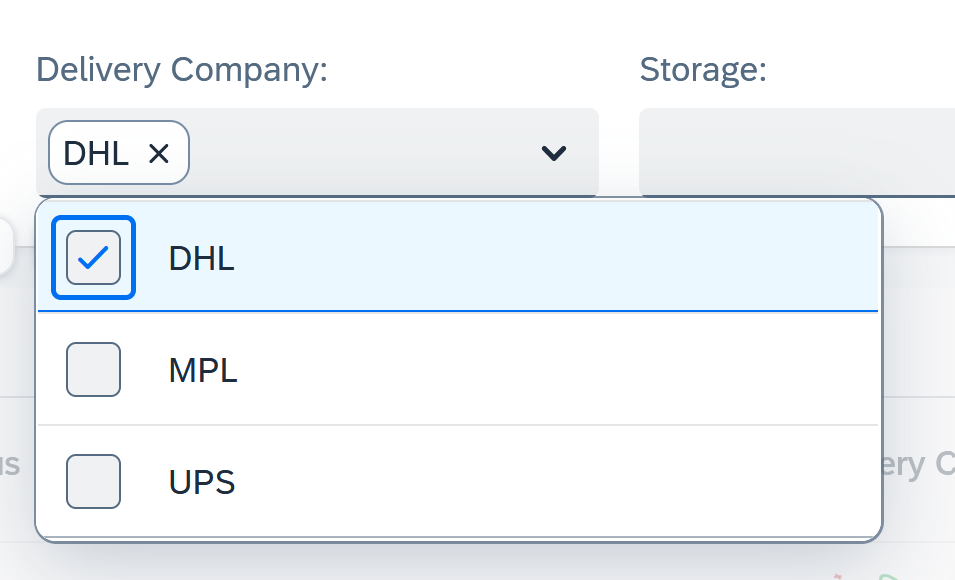
\includegraphics[width=0.45\linewidth]{images/user_doc/managePack/ReportScreen/browse/defaultCompany.png}}

    \subcaptionbox{Storage Filter}{
		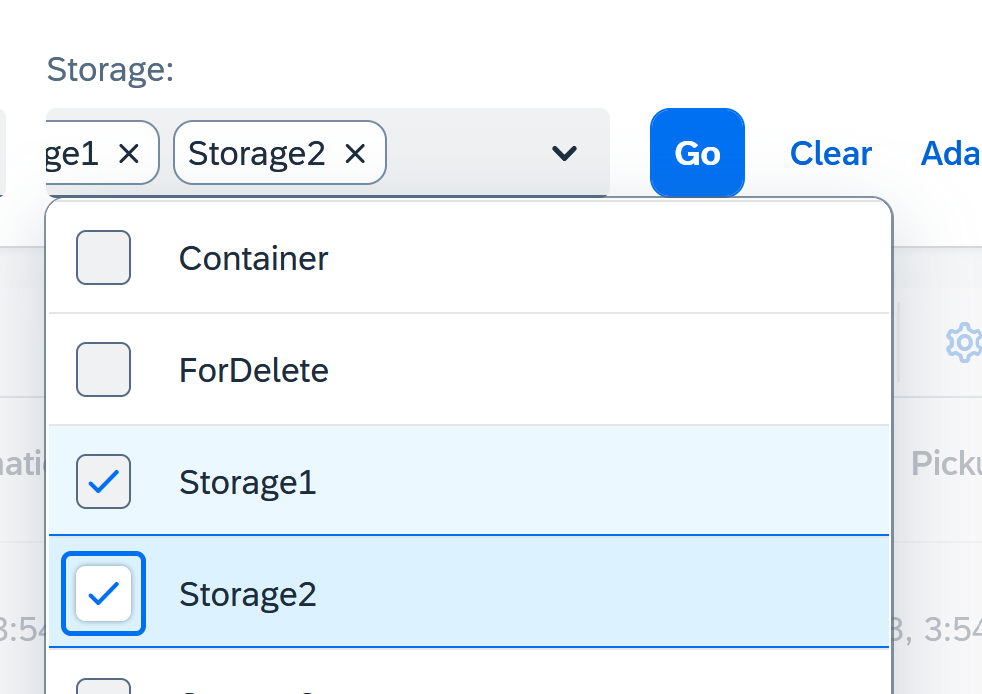
\includegraphics[width=0.45\linewidth]{images/user_doc/managePack/ReportScreen/browse/defaultStorage.png}}
	\caption{Manage Packages Report Screen - Filter Bar - Default Drop Down Filters Show Case}
	\label{fig:MPDefaultDropDown}
\end{figure}

\begin{figure}[H]
		\centering
	\subcaptionbox{While Adjusting the Filter}{
		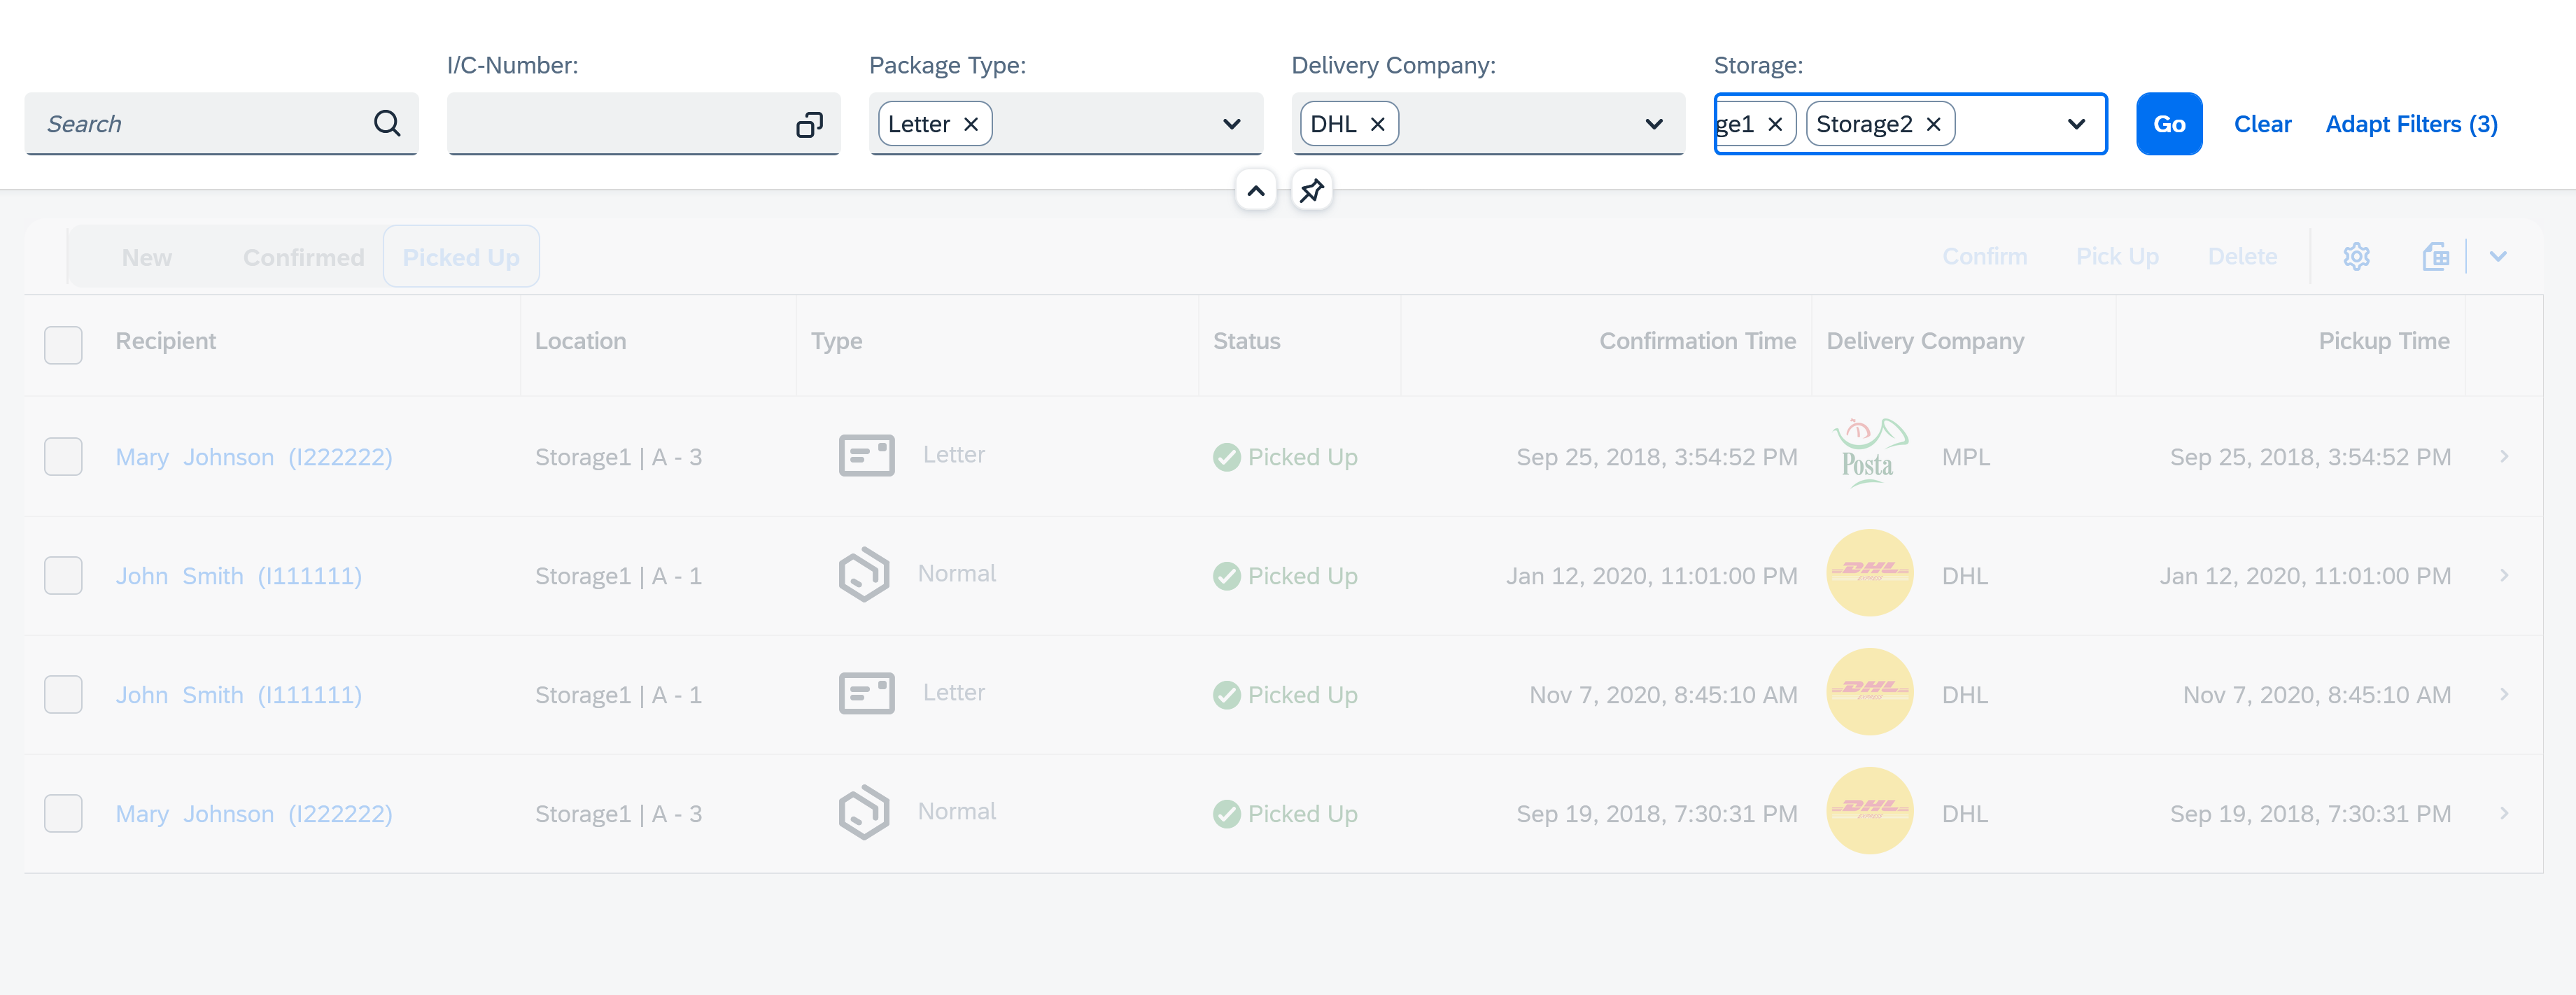
\includegraphics[width=0.45\linewidth]{images/user_doc/managePack/ReportScreen/browse/filterOnAdjusting.png}}
	\hspace{5pt}
	\subcaptionbox{Clicked "Go"}{
		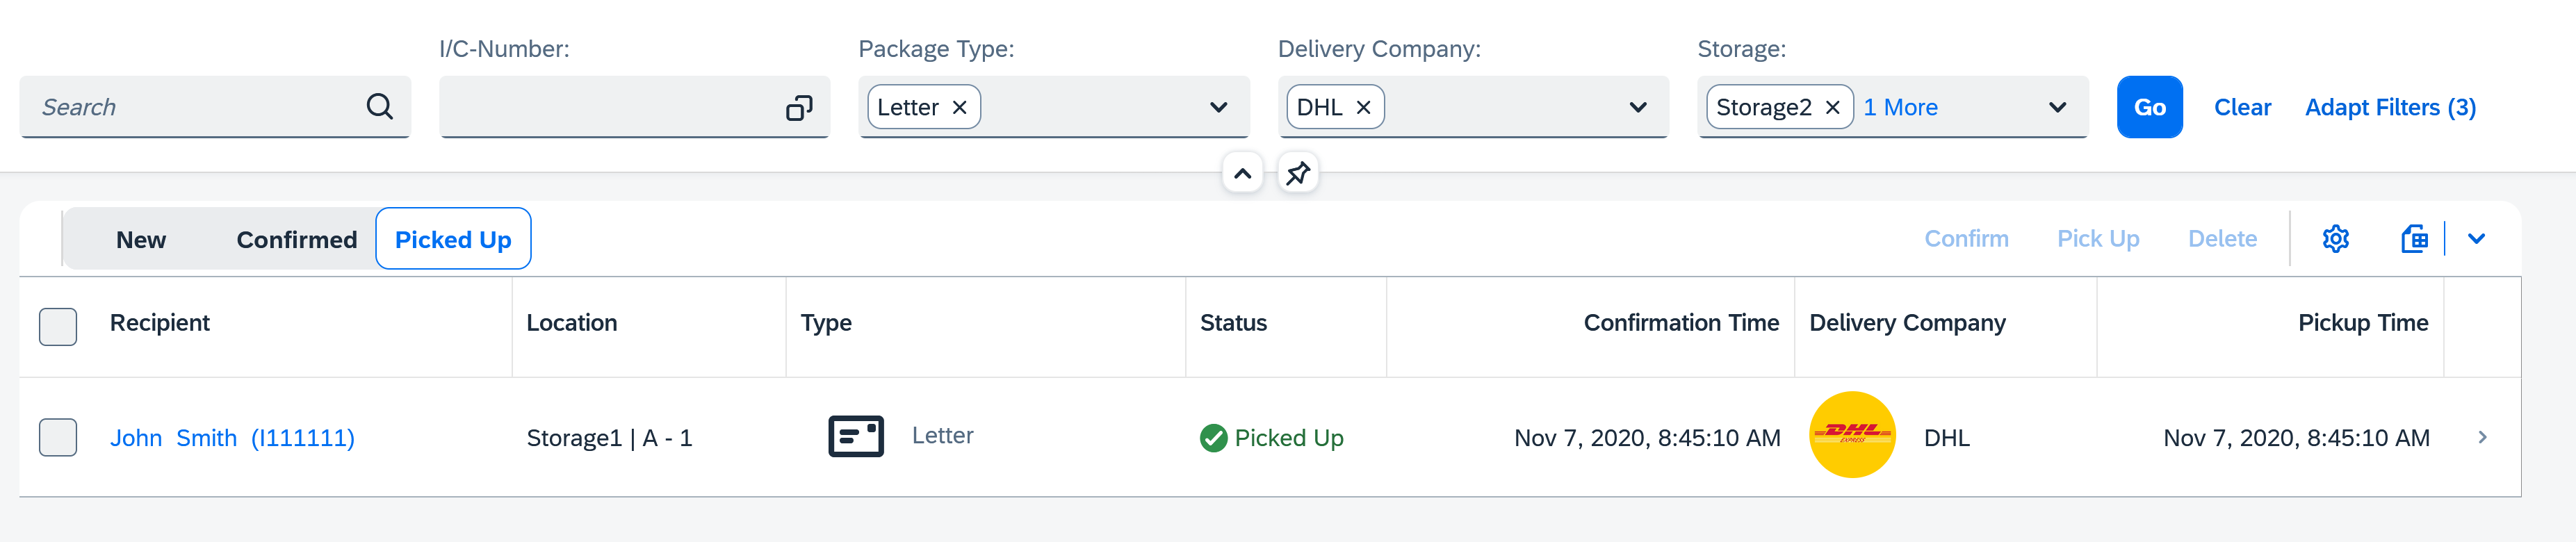
\includegraphics[width=0.45\linewidth]{images/user_doc/managePack/ReportScreen/browse/filterAfterGo.png}}
    \caption{Manage Package Report Screen - Adjust Filters}
    \label{fig:MPAjustFilters}
\end{figure}

In the middle there is a variant bread cum on the left and three action buttons on the right (\autoref{fig:MPMiddle}). The variant breadcrumb shows the three possible status of the packages. When clicking on one of the variants, the list of packages with corresponding status are displayed (\autoref{fig:MPbreadcrumbShowCase}, \autoref{fig:MPBreadCrumb}). The three action buttons are by default inactivated. They will be activated when certain conditions are full filled (i.e. the action can be performed).

\begin{figure}[H]
	\centering
	\subcaptionbox{Variants Bread}{
		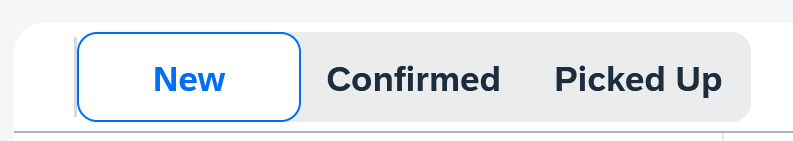
\includegraphics[width=0.45\linewidth]{images/user_doc/managePack/ReportScreen/browse/VariantsBread.png}}
	\hspace{5pt}
	\subcaptionbox{Action Buttons}{
		
\includegraphics[width=0.45\linewidth]{images/user_doc/managePack/ReportScreen/browse/buttonInactive.png}}
  \caption{Manage Packages Report Screen - Middle Control}
	\label{fig:MPMiddle}
\end{figure}

\begin{figure}[H]
	\centering
	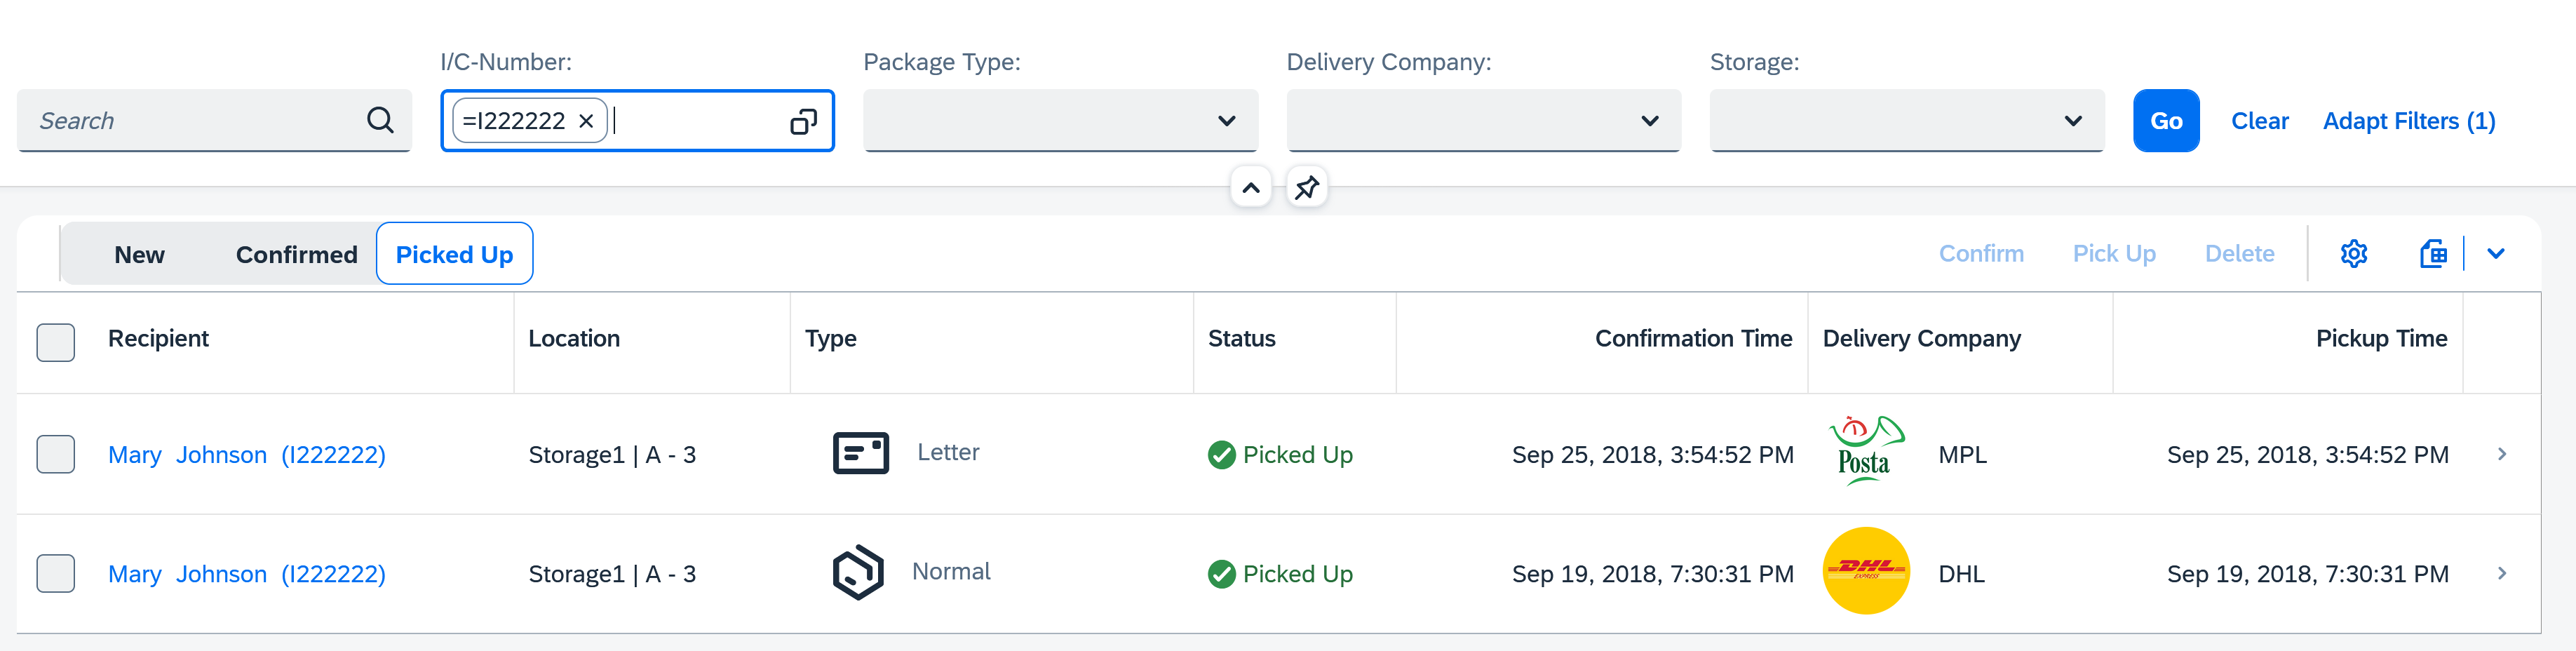
\includegraphics[width=1\linewidth]{images/user_doc/managePack/ReportScreen/browse/defaultFreeTextIdUsage.png}
	\caption{Manage Packages Report Screen - Middle Control - Breadcrumb Show Case}
	\label{fig:MPbreadcrumbShowCase}
\end{figure}


\begin{figure}[H]
	\centering
	\subcaptionbox{New Variant}{
		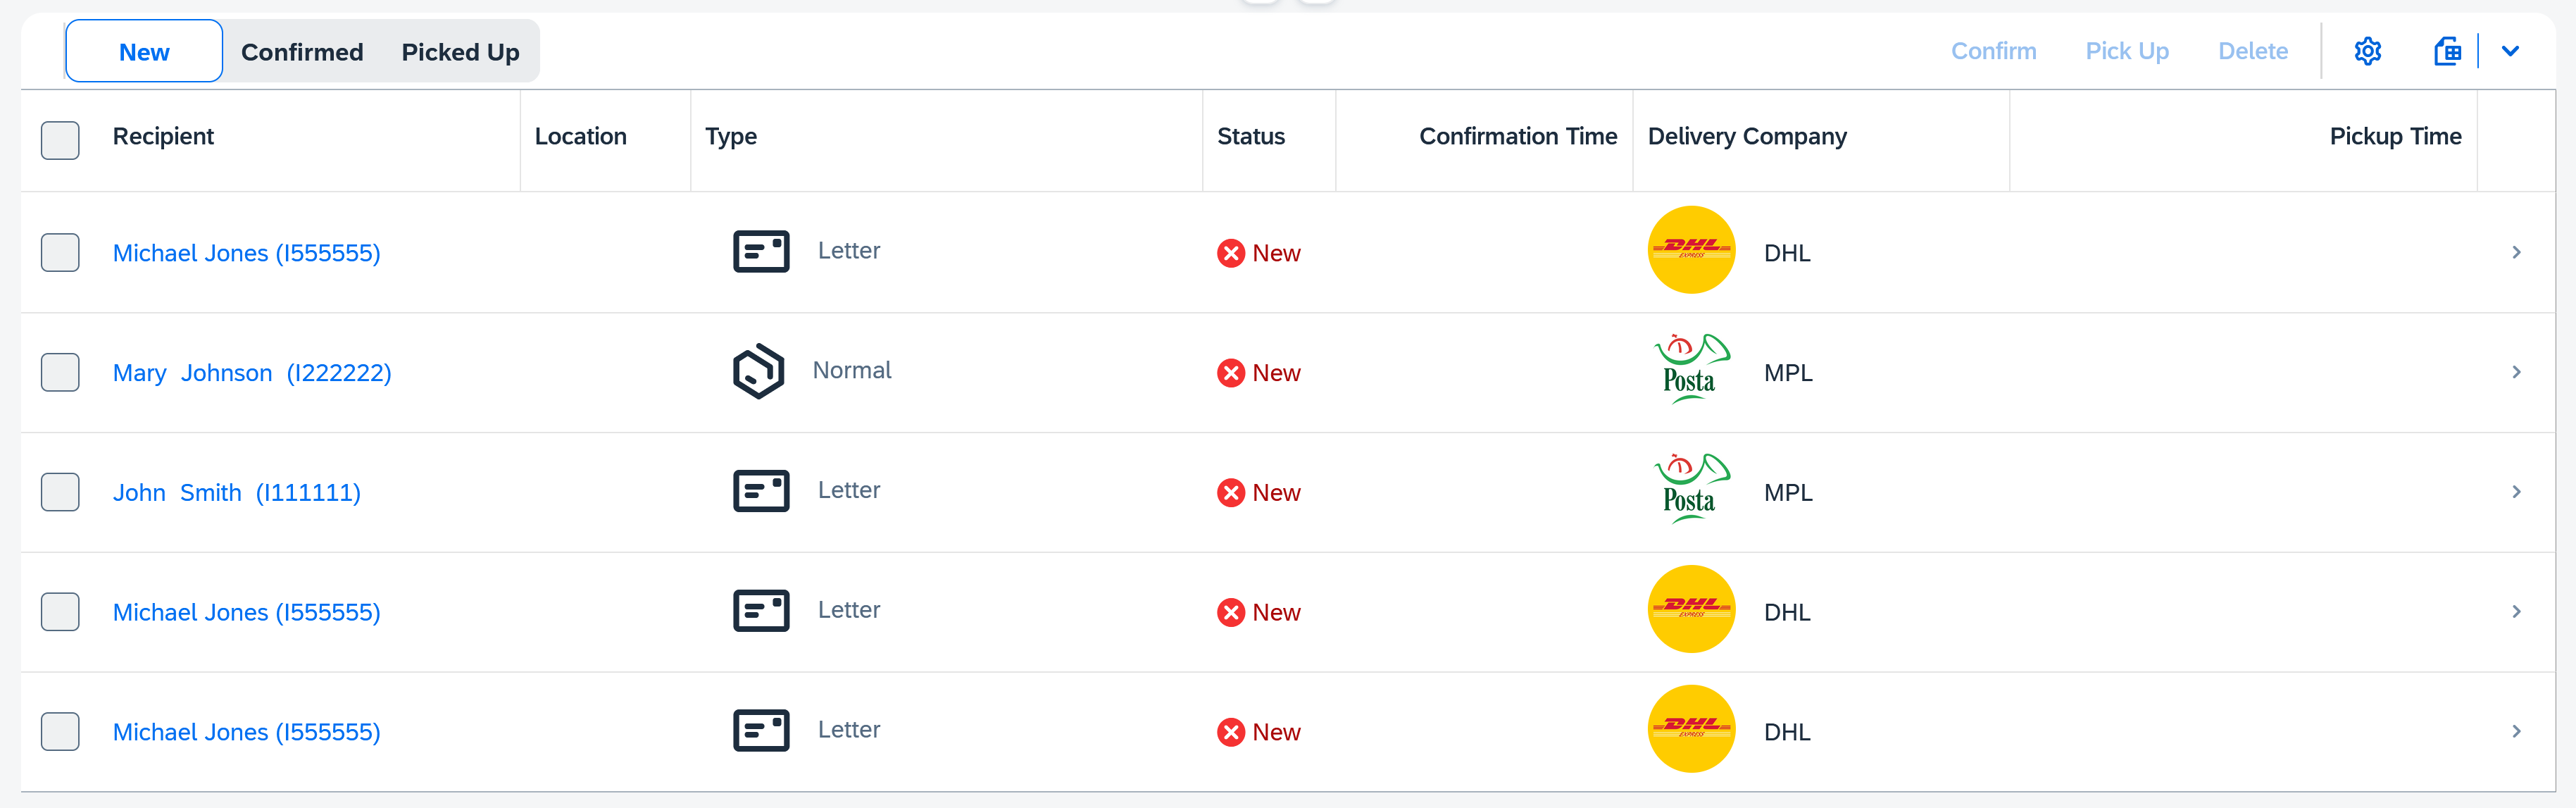
\includegraphics[width=0.45\linewidth]{images/user_doc/managePack/ReportScreen/browse/NewVariant.png}}
	\hspace{5pt}
	\subcaptionbox{Confirmed Variant}{
		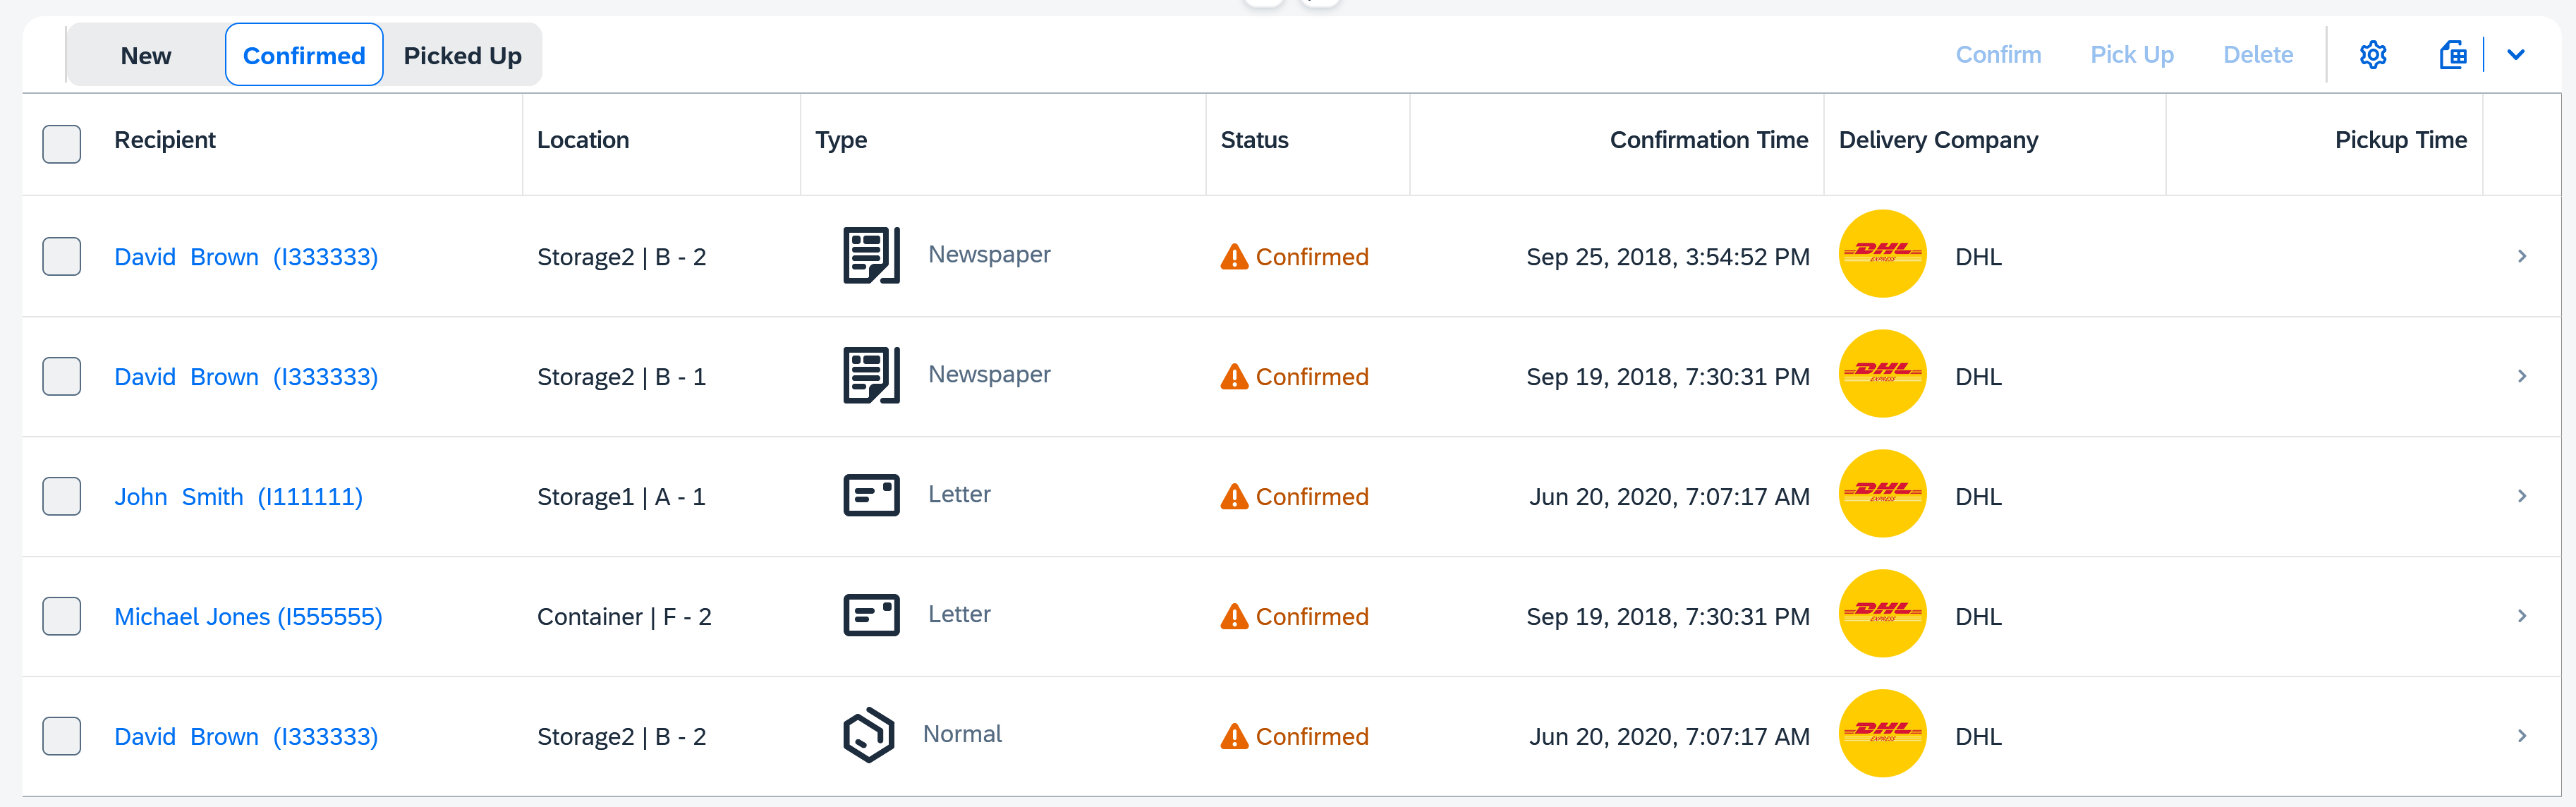
\includegraphics[width=0.45\linewidth]{images/user_doc/managePack/ReportScreen/browse/ConfirmedVariant.png}}

    \subcaptionbox{Picked Up Variant}{
		\includegraphics[width=0.45\linewidth]{images/user_doc/managePack/ReportScreen/browse/pickedupVariant.png}}
	\caption{Manage Packages Report Screen - Middle Control - Breadcrumb Show Case}
	\label{fig:MPBreadCrumb}
\end{figure}

The lower part displays the list of packages. The information provides for each packages are: \textbf{Recipient} (the recipient info, full name and SAP ID), \textbf{Location} (the storage and storage slot info of the package, if applicable), \textbf{Type} (the type of the package, existing types are newspaper, letter and normal), \textbf{Status} (the status of the package, existing status are new, confirmed and picked up), \textbf{Delivery Company} (the delivery company of the package), \textbf{Confirmation Time} (the confirmation time of the package, if applicable), \textbf{Pickup Time} (the picked up time of the package, if applicable).
In case selection of package is needed, one can select a package by ticking the selection box before the listed package item. One can also select and de-select all packages by toggling the selection box at the left corner of the list header (\autoref{fig:MPListSelection}).
In case contact info is needed for certain recipient, one can click at the \textbf{recipient}, a pop up contact card will display the email and phone number of the recipient (\autoref{fig:MPReportCOntactCard}).

\begin{figure}[H]
	\centering
	\subcaptionbox{Select All}{
		\includegraphics[width=0.45\linewidth]{images/user_doc/managePack/ReportScreen/browse/listSelectAll.png}}
	\hspace{5pt}
	\subcaptionbox{Deselect All}{
		\includegraphics[width=0.45\linewidth]{images/user_doc/managePack/ReportScreen/browse/listDeSelectAll.png}}
    \caption{Manage Packages Report Screen - Report List - Selection Show Case}
	\label{fig:MPListSelection}
\end{figure}

\begin{figure}[H]
	\centering
	\includegraphics[height=200pt]{images/user_doc/managePack/ReportScreen/browse/contactcard.png}
	\caption{Manage Packages Report Screen - Report List - Contact Card Show Case}
	\label{fig:MPReportCOntactCard}
\end{figure}

Further details of a package can be obtained by clicking at the package list items. On click, one is navigated to the "Package Detail Screen" displaying \textbf{Basic}, \textbf{General Data} and \textbf{Administrative Data} of the package. (\autoref{fig:MPdetailOverview})

In case the contact info of recipient or receptionist is needed, a contact card can be displayed by clicking on the person. (\autoref{fig:MPObjectContactCard})

\begin{figure}[H]
	\centering
	\includegraphics[height=200pt]{images/user_doc/managePack/DetailScreen/browse/overview.png}
	\caption{Manage Packages Detail Screen - Overview}
	\label{fig:MPdetailOverview}
\end{figure}

\begin{figure}[H]
	\centering
	\subcaptionbox{Receptionist}{
		\includegraphics[width=0.45\linewidth]{images/user_doc/managePack/DetailScreen/browse/contactcard_recep.png}}
	\hspace{5pt}
	\subcaptionbox{Recipient}{
		\includegraphics[width=0.45\linewidth]{images/user_doc/managePack/DetailScreen/browse/contactcard_user.png}}
    \caption{Manage Packages Detail Screen - Contact Card}
	\label{fig:MPObjectContactCard}
\end{figure}

\subsubsection{Confirm Packages}

Confirm a package happens after a \textbf{Receptionist} registered a delivered package when the \textbf{Receptionist} would like to allocate the package a storage slot. Only packages with \textit{new} status can be confirmed. One to many \textit{new} packages can be confirmed at a single time.

The \textbf{Confirm} button at the middle control part is used to trigger the confirm action. It is inactivated until the following conditions are all full filled:

\begin{compactenum}
    \item At the \textbf{New} variant.
    \item At least one \textit{new} package is selected.
\end{compactenum}

\bigskip
Once the \textbf{Receptionist} selected the packages (\autoref{fig:MPReportConfirmBtn}), the \textbf{Confirm} button is activated and clicked, a dialog pops up for the \textbf{Receptionist} to allocate a slot for the package(s) (\autoref{fig:MPReportConfirmDlg}). One should select the storage first from the \textbf{Storage} drop down list and then the slot from the \textbf{Slot} drop down list. The \textbf{Slot} drop down shows always the available slots under the selected storage (\autoref{fig:MPReportConfirmDlgSelection}).

After selected the slot, if one clicks "Close", nothing will happen and dialog will be closed. If one clicks "Save", the packages will be confirmed (i.e. filled with the selected slot info and status changed to confirmed). The dialog will be closed, a message toast indicates the success confirm and the package(s) will be moved from the current \textbf{New} variant to \textbf{Confirmed} Variant. (\autoref{fig:MPReportConfirmDlgButton})

At this point, the package(s) are ready to be picked up, by employee through \textbf{Package Pickup} (\autoref{subsec:pp}) application or by \textbf{Receptionist} using the pickup backup function (\autoref{subsubsec:MPpickup}) of this application.

\bigskip
Note that the confirm action is not irreversible, i.e. a \textit{confirmed} package can no longer be reset to \textit{new} and the confirmed package location can no longer be changed.

\begin{figure}[H]
	\centering
	\includegraphics[width=1\linewidth]{images/user_doc/managePack/ReportScreen/browse/confirmActivated.png}
	\caption{Manage Packages Report Screen - Confirm Step 1 - Select Packages}
	\label{fig:MPReportConfirmBtn}
\end{figure}

\begin{figure}[H]
	\centering
	\includegraphics[height=150pt]{images/user_doc/managePack/ReportScreen/confirm/confirmDialog.png}
	\caption{Manage Packages Report Screen - Confirm Step 2 - Confirm Dialog}
	\label{fig:MPReportConfirmDlg}
\end{figure}

\begin{figure}[H]
	\centering
	\subcaptionbox{Choose Storage}{
		\includegraphics[width=0.45\linewidth]{images/user_doc/managePack/ReportScreen/confirm/confirmStorageDropDown.png}}
	\hspace{5pt}
	\subcaptionbox{Choose Slot}{
		\includegraphics[width=0.45\linewidth]{images/user_doc/managePack/ReportScreen/confirm/confirmSlotDropdown.png}}
    \caption{Manage Packages Report Screen - Confirm Step 3 - Confirm Dialog - Location Selection}
	\label{fig:MPReportConfirmDlgSelection}
\end{figure}

\begin{figure}[H]
	\centering
	\subcaptionbox{Clicked "Save" and Proceeded}{
		\includegraphics[width=0.45\linewidth]{images/user_doc/managePack/ReportScreen/confirm/confirmedToast.png}}
	\hspace{5pt}
	\subcaptionbox{Clicked "Close" and Cancelled}{
		\includegraphics[width=0.45\linewidth]{images/user_doc/managePack/ReportScreen/browse/conifirmClosedClicked.png}}
    \caption{Manage Packages Report Screen - Confirm Step 4 - Confirmed / Cancelled}
	\label{fig:MPReportConfirmDlgButton}
\end{figure}

\subsubsection{Pickup Package}
\label{subsubsec:MPpickup}

Pickup a package happens when the recipients (package owners) came to the reception trying to pickup their confirmed packages and are unable to access the \textbf{Pickup Packages} application on their own. In this case a \textbf{Receptionist} may pickup the package in system on behalf of the recipients. Only packages with \textit{confirmed} status can be confirmed. Only one \textit{confirmed} package at one time can be pickup.

The \textbf{Pickup} button at the middle control part is used to trigger the pickup action. It is inactivated until all the following conditions are full filled:

\begin{compactenum}
    \item At the \textbf{Confirmed} variant.
    \item Exactly one \textit{confirmed} package is selected.
\end{compactenum}

\bigskip
Once the \textbf{Confirm} button is activated (\autoref{fig:MPReportPickupBtn}) and clicked, a warning message box (\autoref{fig:MPReportPickupDlg}) pops up verifying the \textbf{Receptionist}'s intention to mark a package as pickup. If one "OK" is clicked, the packages will be picked up (i.e. status is changed to pickup, all related processes are closed, package logs can no longer be removed from the system). The dialog will be closed, a message toast indicates the success pickup and the package will be moved from the current \textbf{Confirmed} variant to \textbf{Picked Up} Variant. (\autoref{fig:MPReportPickupDlgButton})

\bigskip
Note that the confirm action is not irreversible, i.e. a \textit{picked up} package can no longer be reset to \textit{confirm} or \textit{new}. However, the picked up package's information can still be modified (see \autoref{subsubsec:MPedit}).

\begin{figure}[H]
	\centering
	\includegraphics[width=1\linewidth]{images/user_doc/managePack/ReportScreen/pickup/pickupEnabled.png}
	\caption{Manage Packages Report Screen - Pickup Step 1 - Select Packages}
	\label{fig:MPReportPickupBtn}
\end{figure}

\begin{figure}[H]
	\centering
	\includegraphics[height=100pt]{images/user_doc/managePack/ReportScreen/pickup/pickupDialogOk.png}
	\caption{Manage Packages Pickup Dialog - Pickup Step 2}
	\label{fig:MPReportPickupDlg}
\end{figure}

\begin{figure}[H]
	\centering
	\subcaptionbox{Clicked "OK" and Proceeded}{
		\includegraphics[width=0.45\linewidth]{images/user_doc/managePack/ReportScreen/pickup/pickupToast.png}}
	\hspace{5pt}
	\subcaptionbox{Clicked "Cancel" and Cancelled}{
		\includegraphics[width=0.45\linewidth]{images/user_doc/managePack/ReportScreen/pickup/pickupCanceled.png}}
    \caption{Manage Packages Report Screen - Pickup Step 3 - Pickup / Cancelled}
	\label{fig:MPReportPickupDlgButton}
\end{figure}

\subsubsection{Delete Packages}

Delete a package can be done in two ways: Batch deletions at the "Report Screen" or single deletion at "Detail Screen". Only packages with \textit{confirmed} or \textit{new} status can be deleted. Packages with \textit{picked up} status can no longer be removed. Note that the deletion action is not irreversible.

\bigskip
In case the \textbf{Receptionist} is at "Report Screen" and want to delete one to many package, one can use the "Delete" button at the middle control bar. The "Delete" button is in activated until the following conditions are full filled:

\begin{compactenum}
    \item At the \textbf{Confirmed} or \textbf{New} variant.
    \item At least one package is selected.
\end{compactenum}

\bigskip
Once the \textbf{Delete} button is activated (\autoref{fig:MPReportDeleteBtn}) and clicked, a warning message box (\autoref{fig:MCReportDeleteDlg}) pops up verifying the \textbf{Receptionist}'s intention to delete a package. If one "OK" is clicked, the packages will be deleted (i.e. the package no longer exist in the system). The message box will be closed, a message toast indicates the success deletion and the package will be removed from everywhere. If "Cancel" is clicked, the message box is closed and nothing happens. (\autoref{fig:MPReportDeleteDone})

\begin{figure}[H]
	\centering
	\subcaptionbox{Enabled}{
		\includegraphics[width=0.95\linewidth]{images/user_doc/managePack/ReportScreen/delete/deleteEnabled.png}}

	\subcaptionbox{Disabled for Picked Up Packages}{
		\includegraphics[width=0.95\linewidth]{images/user_doc/managePack/ReportScreen/delete/deleteDisabled.png}}
    \caption{Manage Packages Report Screen - Delete Step 1 - Select Packages}
	\label{fig:MPReportDeleteBtn}
\end{figure}

\begin{figure}[H]
	\centering
	\includegraphics[height=100pt]{images/user_doc/managePack/ReportScreen/delete/deleteDlalog.png}
	\caption{Manage Packages Delete Dialog - Delete Step 2}
	\label{fig:MPReportDeleteDlg}
\end{figure}

\begin{figure}[H]
	\centering
	\includegraphics[height=100pt]{images/user_doc/managePack/ReportScreen/delete/deleteToast.png}
	\caption{Manage Packages Delete Dialog - Delete Step 3 - Deleted}
	\label{fig:MPReportDeleteDone}
\end{figure}


\bigskip
In case the \textbf{Receptionist} is at "Detail Screen" and want to delete the displayed package, the "Delete" button at the top right corner (page header) shall be used. 
The Delete" button is activated if the following conditions are full filled:

\begin{compactenum}
    \item The displayed package is in the status \textbf{new} or \textbf{confirmed}
\end{compactenum}

\bigskip
If the "Delete" button is activated and once clicked, a warning message box pops up verifying the \textbf{Receptionist}'s intention to delete the displayed package. If "Delete" is clicked, the packages will be deleted (i.e. the package no longer exist in the system). The message box will be closed, \textbf{Receptionist} got navigated back to "Report Screen" and a message toast indicates the success deletion. The package will be removed from everywhere. If "Cancel" is clicked, the message box is closed and nothing happens. (\autoref{fig:MPDetailDeleteGuide})

\begin{figure}[H]
	\centering
    \vspace{5pt}
	\subcaptionbox{Step 1: Deletion Enabled for Non-picked Up Packages}{
		\includegraphics[width=0.95\linewidth]{images/user_doc/managePack/DetailScreen/delete/deleteEnabled2.png}}
    \vspace{10pt}
	\subcaptionbox{Step 2: Deletion Verification}{
		\includegraphics[height=150pt]{images/user_doc/managePack/DetailScreen/delete/deleteDialog2.png}}
    \vspace{10pt}
    \subcaptionbox{Step 3: Navigated Back}{
		\includegraphics[width=1\linewidth]{images/user_doc/managePack/ReportScreen/delete/deleteToast.png}}
    \caption{Manage Packages Detail Screen - Delete Package Guide}
	\label{fig:MPDetailDeleteGuide}
\end{figure}

\subsubsection{Edit Package}
\label{subsubsec:MPedit}

Edit a package can be done at "Detail Screen".
In case the \textbf{Receptionist} is at "Detail Screen" and want to edit the displayed package, one can use the "Edit" button at top right corner (page header). 
When the "Edit" button is clicked, a editing dialog pops up, allowing \textbf{Receptionist} to modified the \textbf{Recipient}, \textbf{Type}, \textbf{Delivery Company}, \textbf{Comment} of the package. (\autoref{fig:MPDetailEditBtn})
When click "Save", the modified details are submitted, the dialog closes, a message toast pops up indicating the success and the changes reflects ont the "Detail Screen". When click "Close", any changes will be discard, the dialog simply closes.
(\autoref{fig:MPReportEditDone}

\begin{figure}[H]
	\centering
    \vspace{5pt}
	\subcaptionbox{Step 1: Edit Dialog}{
		\includegraphics[width=0.45\linewidth]{images/user_doc/managePack/DetailScreen/edit/editDialog.png}}
    \hspace{5pt}
    \subcaptionbox{Step 2: Modify Recipient}{
		\includegraphics[width=0.45\linewidth]{images/user_doc/managePack/DetailScreen/edit/editSelection1.png}}
	\subcaptionbox{Step 3: Modify Type}{
		\includegraphics[width=0.45\linewidth]{images/user_doc/managePack/DetailScreen/edit/editSelection2.png}}
    \hspace{5pt}
    \subcaptionbox{Step 4: Modify Delivery Company}{
		\includegraphics[width=0.45\linewidth]{images/user_doc/managePack/DetailScreen/edit/editSelection3.png}}
    \caption{Manage Packages Detail Screen - Edit Dialog Guide}
	\label{fig:MPDetailEditBtn}
\end{figure}


\begin{figure}[H]
	\centering
	\includegraphics[width=1\linewidth]{images/user_doc/managePack/DetailScreen/edit/editToast.png}
	\caption{Manage Packages Detail Screen - Edited}
	\label{fig:MPReportEditDone}
\end{figure}

\pagebreak

\section{Facility Manager}
\label{sec:UdocFacilityManager}

As a logged in \textbf{Facility Manager} (See \autoref{sec:GeneralRequisite} for all possible roles, one is granted to access the two applications under the \textbf{Administration} section, namely \textbf{Manage Companies} (\autoref{subsec:mc}) and \textbf{Manage Storage} (\autoref{subsec:ms}). One can quick jump to the section by left clicking the "Administration" tab. One can enter the application by left click the tiles. (\autoref{fig:ManagerApplications})

\begin{figure}[H]
	\centering
	\includegraphics[width=1\linewidth]{images/user_doc/overviews/AdminTab.png}
	\caption{Facility Management Applications}
	\label{fig:ManagerApplications}
\end{figure}


\subsection{Manage Companies}
\label{subsec:mc}

The \textbf{Manage Companies} application is used by \textbf{Facility Manager} (in short \textbf{FM}) maintaining the information of potential delivery companies delivering the package in the system. For each delivery company, its name, optionally a logo and the administration data (creation time, creation user, last modified time, last modified user) are stored. The administration data are auto maintained and is not editable by the \textbf{FM}. The summarized main actions the \textbf{FM} can take within the application are listed here:

\begin{compactenum}
	\item Browse the delivery companies.
        \begin{compactenum}
            \item Filtering possibility.
            \item Report List of delivery companies info.
            \item Detail page for single delivery company.
        \end{compactenum}
    \item Add new delivery companies. (name and logo)
    \item Edit existing delivery companies (name and logo).
    \item Delete package(s) which status is new or confirmed.
\end{compactenum}

\subsubsection{Browse}
As an \textbf{FM}, after clicking at the application tile, is redirected to the "Report Screen", which is the main screen of the application. (\autoref{fig:CompanyOverview})

\begin{figure}[H]
	\centering
	\includegraphics[width=1\linewidth]{images/user_doc/company/report/overview.png}
	\caption{Manage Companies - Overview}
	\label{fig:CompanyOverview}
\end{figure}

The upper part displays the search bar and the possible filters. 
In case the need of free text search of any possible content of the column, one can use the \textbf{"Search Bar"}. The search supports in-completed keywords and is case insensitive. One can also use the fixed filters for administration data. "Created By" and "Last Updated By" accepts free text of any valid SAP ID. "Created On" and "Last Updated On" requires entries of time stamps. \textbf{FM} can click at the double square at the right of input bar to open a filter help dialog, where specific criteria (e.g. between, equal, contains, etc.) can be chosen and a time entry clock can be used to enter time stamps. (\autoref{fig:CompanyOverview})

When adjusting the filtering values, the list view is temporarily locked. After adjusting the filtering values, one can run and review the filter result by clicking the "Go" button or hit "Enter" on keyboard. In case a company is edited and the table content is not reflected, click the "Go" button or hit "Enter" on keyboard to refresh. (\autoref{fig:CompanyOverview})

The lower part displays the list of delivery companies. In the list header, number of total delivery companies in the list is displayed on the left and two action buttons, "Create" and "Delete" are placed on the right. (\autoref{fig:CompanyOverview})

The information provides for each delivery companies in the list body (table) are: \textbf{Delivery Company} (company name with logo), \textbf{Created On} (the creation time of the company), \textbf{Created By} (the company creator's SAP ID). (\autoref{fig:CompanyOverview})

In case selection of package is needed, one can select a package by ticking the selection box before the listed package item. One can also de-select all packages by clicking at the selection box at the left corner of the table header. (\autoref{fig:CompanyOverview})

\bigskip

When the \textbf{FM} click at one item of the table, the \textbf{FM} is redirected to the "Detail Screen" displays the details of the selected item. (\autoref{fig:MCdetailOVerview})

\begin{figure}[H]
	\centering
	\includegraphics[width=1\linewidth]{images/user_doc/company/detail/DetailOverview.png}
	\caption{Manage Company Detail Screen - Overview}
	\label{fig:MCdetailOVerview}
\end{figure}

The "Detail Screen" displays the company name as the title on the left and two action buttons, "Delete" and "Edit" at the right in the header, and its full administration data in the body. (\autoref{fig:MCdetailOVerview})

\subsubsection{Add}

\textbf{FM} can add new delivery company to the system at "Report Screen" by clicking the "Create" button. 
When the "Create" button is clicked, a creation dialog pops up, where the \textbf{Name} and the \textbf{Logo} info of the company should be entered. The \textbf{Name} waits for input of free text of the company name and should not be left empty. The \textbf{Logo} waits for input of free text of a url to the image of the company's logo and can be left empty. (\autoref{fig:MCreportCreateGuide} - a,b)

After filling the dialog form, if "Create" is clicked, the entered info will be submitted, the dialog will be closed, a success message toast is displayed and the entered company appears in the table on the "Report Screen". If "Cancel" is clicked, the dialog will be closed, entered data is discarded and nothing happens. (\autoref{fig:MCreportCreateGuide} - c)

\begin{figure}[H]
	\centering
	\subcaptionbox{Step 1: Create Dialog}{
		\includegraphics[width=0.45\linewidth]{images/user_doc/company/report/createDlg.png}}
    \hspace{5pt}
    \subcaptionbox{Step 2: Data Entry}{
		\includegraphics[width=0.45\linewidth]{images/user_doc/company/report/createDlgEntries.png}}
    \vspace{10pt}
   \subcaptionbox{Step 3: Post Creation}{
		\includegraphics[width=1\linewidth]{images/user_doc/company/report/createdToast.png}}
    \caption{Manage Company Report Screen - Create Dialog Guide}
	\label{fig:MCreportCreateGuide}
\end{figure}

\subsubsection{Edit Company}

Edit a delivery company can be done at "Detail Screen" by the \textbf{FM}.
\bigskip

In case the \textbf{FM} is at "Detail Screen" and want to edit the displayed company, the \textbf{FM} can use the "Edit" button at top right corner (page header). 
When the "Edit" button is clicked, a editing dialog pops up, allowing \textbf{FM} to modified the \textbf{Name}, \textbf{Logo} of the company. Initially the fields are filled with current data of the company. The \textbf{Name} should contain free text of the company's name and should not be left empty. The \textbf{Logo} should contain free text of a url to the logo image and can be left empty.
When click "Save", the modified details are submitted, the dialog closes, a message toast pops up indicating the success and the changes reflects on the "Detail Screen". When click "Close", any changes will be discard, the dialog simply closes. (\autoref{fig:MCDetailEditGuide}, \autoref{fig:MCDetailEditDlgBad})

\begin{figure}[H]
	\centering
    \vspace{5pt}
	\subcaptionbox{Step 1: Edit Dialog}{
		\includegraphics[width=0.35\linewidth]{images/user_doc/company/detail/EditDlg.png}}
    \hspace{5pt}
    \subcaptionbox{Step 2: Post Success Edit}{
		\includegraphics[width=0.55\linewidth]{images/user_doc/company/detail/EditToast.png}}
    \caption{Manage Company Detail Screen - Edit Dialog Guide}
	\label{fig:MCDetailEditGuide}
\end{figure}

\begin{figure}[H]
	\centering
    \vspace{5pt}
	\subcaptionbox{Empty Company Name}{
		\includegraphics[width=0.35\linewidth]{images/user_doc/company/detail/EditBadInput.png}}
    \hspace{5pt}
    \subcaptionbox{Step 2: Error Message}{
		\includegraphics[width=0.55\linewidth]{images/user_doc/company/detail/editBadInputErrorMsg.png}}
    \caption{Manage Companies Detail Screen - Edit Dialog - Bad Inputs Example}
	\label{fig:MCDetailEditDlgBad}
\end{figure}

\subsubsection{Delete Company}

Delete an existing delivery company can be done in two ways: Batch deletions at the "Report Screen" or single deletion at "Detail Screen". The deletion of a company implies that, the delivery company will be removed completely and any association of existing packages to this company is automatically removed as well. This means those packages will no longer holds any company information. The deletion action is irreversible. 

In case the \textbf{FM} is at "Report Screen" and want to delete one to many companies, one can use the "Delete" button at the list header. The "Delete" button is inactivated until the following conditions are full filled:

\begin{compactenum}
    \item At least one delivery company is selected.
\end{compactenum}

Once the \textbf{Delete} button is activated and clicked, a warning message box pops up verifying the \textbf{FM}'s intention to delete a package. If "OK" is clicked, the company(s) will be deleted. The message box will be closed, a message toast indicates the success deletion and the package will be removed from everywhere. If "Cancel" is clicked, the message box is closed and nothing happens.
(\autoref{fig:MCReportDeleteStep1}, \autoref{fig:MCReportDeleteDlg}, 
\autoref{fig:MCReportDeleteStep3})

\begin{figure}[H]
	\centering
	\includegraphics[width=0.90\linewidth]{images/user_doc/company/report/deleteBtnEnable.png}
	\caption{Manage Companies - Delete - Step 1: Select Company to Delete}
	\label{fig:MCReportDeleteStep1}
\end{figure}

\begin{figure}[H]
	\centering
	\includegraphics[height=100pt]{images/user_doc/company/report/deleteConfirmaton2.png}
	\caption{Manage Companies - Delete - Step 2: Delete Dialog}
	\label{fig:MCReportDeleteDlg}
\end{figure}

\begin{figure}[H]
	\centering
	\includegraphics[width=0.90\linewidth]{images/user_doc/company/report/deleteToast.png}
	\caption{Manage Companies - Delete - Step 3: Post Delete}
	\label{fig:MCReportDeleteStep3}
\end{figure}

\bigskip
In case the \textbf{FM} is at "Detail Screen" and want to delete the displayed company, the "Delete" button at the top right corner (page header) shall be used. 

Once clicked, a warning message box pops up verifying the \textbf{FM}'s intention to delete the displayed company. If "Delete" is clicked, the company will be deleted. The message box will be closed, \textbf{FM} got navigated back to "Report Screen" and a message toast indicates the success deletion. If "Cancel" is clicked, the message box is closed and nothing happens. (\autoref{fig:MCDetailDeleteGuide})

\begin{figure}[H]
	\centering
	\subcaptionbox{Step 1: Deletion Verification When Clicked "Delete"}{
		\includegraphics[height=150pt]{images/user_doc/company/detail/deleteConfirmation.png}}
    \vspace{10pt}
	\subcaptionbox{Step 2: Navigated Back After Deletion}{
		\includegraphics[width=1\linewidth]{images/user_doc/company/detail/AfterDeletionBack.png}}
    \caption{Manage Companies Detail Screen - Delete Company Guide}
	\label{fig:MCDetailDeleteGuide}
\end{figure}



\subsection{Manage Storage}
\label{subsec:ms}

The \textbf{Manage Storage} application is used by \textbf{Facility Manager} (in short \textbf{FM}) maintaining the information of potential storage places and storage slots within certain storage holding the package in the system.  
The summarized main actions the \textbf{FM} can take within the application are listed here:

\begin{compactenum}
	\item Browse the storage and slots in the storage.
        \begin{compactenum}
            \item Filtering possibility.
            \item Report List of storage.
            \item Detail page for storage.
            \item Detail page for slot.
        \end{compactenum}
    \item Add new storage.
        \begin{compactenum}
            \item At Storage Report Page.
        \end{compactenum}
    \item Edit existing storage.
        \begin{compactenum}
            \item At Storage Detail Page.
        \end{compactenum}
    \item Delete existing storage.
        \begin{compactenum}
            \item At Storage Report Page.
            \item At Storage Detail Page.
        \end{compactenum}
    \item Add new storage slot.
        \begin{compactenum}
            \item At Storage Detail Page.
        \end{compactenum}
    \item Batch add new storage slots.
        \begin{compactenum}
            \item At Storage Detail Page.
        \end{compactenum}
    \item Edit existing storage slot.
        \begin{compactenum}
            \item At Slot Detail Page.
        \end{compactenum}
    \item Delete existing storage slot.
        \begin{compactenum}
            \item At Slot Detail Page.
            \item At Storage Detail Page.
        \end{compactenum}
\end{compactenum}

\subsubsection{Browse}

As an \textbf{FM}, after clicking at the application tile, is redirected to the "Storage Report Screen", which is the main screen of the application. (\autoref{fig:MSstorageReportPage})

\begin{figure}[H]
	\centering
	\includegraphics[width=1\linewidth]{images/user_doc/storage/StorageReportPage/reportDefaultOverview.png}
	\caption{Manage Storage - Storage Report Screen}
	\label{fig:MSstorageReportPage}
\end{figure}

The upper part displays the search bar and the possible filters. 
In case the need of free text search of any possible content of the column, one can use the \textbf{"Search Bar"}. The search supports in-completed keywords and is case insensitive. 
\textbf{FM} can also use the default filters, "Building Floor" and "Building", which are two drop down of all available building floors and buildings. \textbf{FM} may use the "Adapt Filter" option (right most of the filter bar), through which \textbf{FM} can add more filters options onto the filter bar.
(\autoref{fig:MSstReportFilterBar}, 
\autoref{fig:MSstorageReportFilterDefault}, 
\autoref{fig:MSstorageReportFilterAdaption})

\begin{figure}[H]
	\centering
	\includegraphics[width=1\linewidth]{images/user_doc/storage/StorageReportPage/reportFilterBar.png}
	\caption{Manage Storage Storage Report Screen - Filter Bar}
	\label{fig:MSstReportFilterBar}
\end{figure}

\begin{figure}[H]
	\centering
	\subcaptionbox{Drop Down of All Possible Building Floor Options}{
		\includegraphics[width=0.45\linewidth]{images/user_doc/storage/StorageReportPage/defaultFIlterBF.png}}
    \hspace{5pt}
    \subcaptionbox{Drop Down of All Possible Building Options}{
		\includegraphics[width=0.45\linewidth]{images/user_doc/storage/StorageReportPage/defaultFIlterBD.png}}
    \caption{Manage Storage Storage Report Screen - Filter Drop down Show Case}
	\label{fig:MSstorageReportFilterDefault}
\end{figure}

\begin{figure}[H]
	\centering
	\subcaptionbox{Option Dialog 1: Simple List}{
		\includegraphics[width=0.45\linewidth]{images/user_doc/storage/StorageReportPage/filterOption.png}}
    \hspace{5pt}
    \subcaptionbox{Option Dialog 2: Grouped}{
		\includegraphics[width=0.45\linewidth]{images/user_doc/storage/StorageReportPage/filterOption2.png}}

    \vspace{10pt}
	\subcaptionbox{After Filter Adaption}{
		\includegraphics[width=1\linewidth]{images/user_doc/storage/StorageReportPage/filterAdaption.png}}
    \caption{Manage Storage Storage Report Screen - Filter Adaption Guide}
	\label{fig:MSstorageReportFilterAdaption}
\end{figure}

When adjusting the filtering values, the list view is temporarily locked. After adjusting the filtering values, one can run and review the filter result by clicking the "Go" button or hit "Enter" on keyboard. In case a storage is edited or deleted and the table content is not reflected, click the "Go" button or hit "Enter" on keyboard to refresh and get the freshest storage info. 
(\autoref{fig:MSstorageReportFilterLock})

\begin{figure}[H]
	\centering
    \vspace{5pt}
	\subcaptionbox{While Adjusting the Filters the Storage List is Locked}{
		\includegraphics[width=0.45\linewidth]{images/user_doc/storage/StorageReportPage/listLock.png}}
    \hspace{5pt}
    \subcaptionbox{Clicked "Go" to Display the Filtering Results}{
		\includegraphics[width=0.45\linewidth]{images/user_doc/storage/StorageReportPage/filterAfterGo.png}}
    \caption{Manage Storage Storage Report Screen - Filter Lock}
	\label{fig:MSstorageReportFilterLock}
\end{figure}

\bigskip

The lower part displays the list report of storage. In the list header, number of total storage in the list is displayed on the left and two action buttons, "Create" and "Delete", and a table column "setting" (icon) are placed on the right. (\autoref{fig:MSrl})

The default columns provides for each storage in the list body (table) are: \textbf{Name} (storage name), \textbf{Location} (the building floor the storage located on), \textbf{Location Instructions} (any helping info regarding the location of the storage), \textbf{Total Number of Packages} (the total number of the packages that had been confirmed in this storage since its creation), \textbf{Current Utilizations} (the number of packages that are currently confirmed in this storage), \textbf{Map} (a link, on click opens a new tab to the map of the location of the storage). 
(\autoref{fig:MSrl})

\textbf{FM} may add more columns to the table by clicking the "setting" icon on the list header. A column adaption dialog will pop up for the \textbf{FM} to select the columns to show.
(\autoref{fig:MSstorageReportColumnAdaption})

\begin{figure}[H] % Storage List
	\centering
	\includegraphics[width=1\linewidth]{images/user_doc/storage/StorageReportPage/reportList.png}
	\caption{Manage Storage Storage Report Screen - Storage List}
	\label{fig:MSrl}
\end{figure}

\begin{figure}[H] % MSstorageReportColumnAdaption
	\centering
	\subcaptionbox{Step 1: column "setting"}{
		\includegraphics[width=0.45\linewidth]{images/user_doc/storage/StorageReportPage/columnSettings.png}}
    \hspace{5pt}
	\subcaptionbox{Step 2: Column Selection Dialog}{
		\includegraphics[width=0.45\linewidth]{images/user_doc/storage/StorageReportPage/columnAdaptionDlg.png}}
    
    \vspace{10pt}
    \subcaptionbox{Step 3: Selected Columns Displayed}{
        \includegraphics[width=0.95\linewidth]{images/user_doc/storage/StorageReportPage/columnMOre.png}}
    \caption{Manage Storage Storage Report Screen - Column Adaption Guide}
	\label{fig:MSstorageReportColumnAdaption}
\end{figure}

In case selection of storage is needed, \textbf{FM} can select a package by ticking the selection box before the listed storage item. One can also deselect all storage by clicking at the selection box at the left corner of the table header.

\bigskip

When the \textbf{FM} click at one item of the table, the \textbf{FM} is redirected to the "Storage Detail Screen".
(\autoref{fig:MSdetailOVerview})

\begin{figure}[H]
	\centering
	\includegraphics[width=1\linewidth]{images/user_doc/storage/StorageReportPage/storageObjWithSlots.png}
	\caption{Manage Storage Storage Detail Screen - Overview}
	\label{fig:MSdetailOVerview}
\end{figure}

The header part of "Storage Detail Screen" displays the storage name as the title and location instruction as description on the left and two action buttons, "Delete" and "Edit" at the right.
Under the title it displays important info of the storage (location, total utilization, current utilization and map). On click the map, the \textbf{FM} will be redirected out of the application to the map of the storage.
(\autoref{fig:MSstorageObjHeader})

\begin{figure}[H] % StorageObjHeader
	\centering
	\includegraphics[width=1\linewidth]{images/user_doc/storage/StorageObjectPage/StorageObjHeader.png}
	\caption{Manage Storage Storage Detail Screen - Header}
	\label{fig:MSstorageObjHeader}
\end{figure}

The bottom body part displays the list of slots contained by the given storage. The list of slots displays the following columns / information: \textbf{Name} (slot name), \textbf{Total Number of Packages} (total number of the packages stored in the slot since its creation date), \textbf{status} (the status of the slot). The availiable status of the slot are: inuse (indicates there is currently at least one package stored inside), empty (indicates there is no package inside) and unavailable (indicates the slot cannot be used due to some reasons).
(\autoref{fig:MSstorageObjSlotList})
In case a slot is edited and the table content is not reflected, refresh the entire page.

\begin{figure}[H] % slotList
	\centering
	\includegraphics[width=1\linewidth]{images/user_doc/storage/StorageObjectPage/slotList.png}
	\caption{Manage Storage Storage Detail Screen - Slot List}
	\label{fig:MSstorageObjSlotList}
\end{figure}

\bigskip

When the \textbf{FM} clicks on one slot item in the slot list, the \textbf{FM} is redirected to slot's "Slot Detail Page". 
(\autoref{fig:MSslotObjOverview})

\begin{figure}[H] % slotObjOverview
	\centering
	\includegraphics[width=1\linewidth]{images/user_doc/storage/SlotObjectPage/slotObjOverview.png}
	\caption{Manage Storage Slot Detail Screen}
	\label{fig:MSslotObjOverview}
\end{figure}


\subsubsection{Add Storage}

\textbf{FM} can add new storage to the system at "Report Screen" by clicking the "Create" button.
When the "Create" button is clicked, a creation dialog pops up. The \textbf{Name} waits for input of free text of the storage and should not be left empty. The \textbf{Map} waits for input of free text of a url to the location of the storage and can be left empty. The \textbf{Location Instruction} waits for input of free text and can be left empty.
(\autoref{fig:MSreportCreateGuide})

After filling the dialog form, if "Create" is clicked, the entered info will be submitted, the dialog will be closed, a success message toast is displayed and the entered storage appears in the table on the "Report Screen". If "Cancel" is clicked, the dialog will be closed, entered data is discarded and nothing happens.
(\autoref{fig:MSreportCreateGuide})

\begin{figure}[H]
	\centering
	\subcaptionbox{Step 1: Open Create Dialog}{
		\includegraphics[width=0.45\linewidth]{images/user_doc/storage/StorageReportPage/createStorageDlg.png}}
    \hspace{5pt}
    \subcaptionbox{Step 2.1: Data Entry - Select Building Floor}{
		\includegraphics[width=0.45\linewidth]{images/user_doc/storage/StorageReportPage/csdlgDropDown.png}}
  
    \vspace{10pt}
    \subcaptionbox{Step 2.2: Data Entry - Bad Input Warning Example}{
		\includegraphics[width=0.45\linewidth]{images/user_doc/storage/StorageReportPage/csdlgBadInput.png}}
    \hspace{5pt}
    \subcaptionbox{Step 2.2: Data Entry - Filled}{
		\includegraphics[width=0.45\linewidth]{images/user_doc/storage/StorageReportPage/csdlgFilled.png}}

    \vspace{10pt}
    \subcaptionbox{Step 3: Post Creation}{
		\includegraphics[width=1\linewidth]{images/user_doc/storage/StorageReportPage/createdToast.png}}
    
    \caption{Manage Storage Storage Report Screen - Create Storage Dialog Guide}
	\label{fig:MSreportCreateGuide}
\end{figure}


\subsubsection{Edit Storage}

\textbf{FM} can edit a storage at "Storage Detail Screen".
In case the \textbf{FM} is at "Storage Detail Screen" and want to edit the displayed company, the \textbf{FM} can use the "Edit" button at top right corner (page header). 
When the "Edit" button is clicked, a editing dialog pops up, allowing \textbf{FM} to modified the \textbf{Name}, \textbf{Building Floor}, \textbf{Map}, \textbf{Location Instructions} of the company. Initially the fields are filled with current data of the storage. The entry rules are the same as creating the storage.
When click "Save", the modified details are submitted, the dialog closes, a message toast pops up indicating the success and the changes reflects on the "Storage Detail Screen". When click "Close", any changes will be discard, the dialog simply closes.
(\autoref{fig:MSDetailEditBtn})

\begin{figure}[H]
	\centering
    \vspace{5pt}
	\subcaptionbox{Step 1: Edit Dialog}{
		\includegraphics[width=0.30\linewidth]{images/user_doc/storage/StorageObjectPage/storageEditDlg.png}}
    \hspace{5pt}
    \subcaptionbox{Step 2: Post Success Edit}{
		\includegraphics[width=0.60\linewidth]{images/user_doc/storage/StorageObjectPage/storageEditedToast.png}}
    \caption{Manage Storage Storage Detail Screen - Edit Dialog Guide}
	\label{fig:MSDetailEditBtn}
\end{figure}

\subsubsection{Delete Storage}

\textbf{FM} can delete a storage in two ways: Batch deletions at the "Storage Report Screen" or single deletion at "Storage Detail Screen". 
The deletion of a storage implies that, the storage will be removed completely from the system. The deletion action is irreversible. 

In case the \textbf{FM} is at "Storage Report Screen" and want to delete one to many storage, the \textbf{FM} can use the "Delete" button at the list header. The "Delete" button is in activated until the following conditions are full filled:

\begin{compactenum}
    \item At least one storage is selected.
\end{compactenum}

Once the \textbf{Delete} button is activated and clicked, a warning message box pops up verifying the \textbf{FM}'s intention to delete a storage. If one "Delete" is clicked, the selected storage will be deleted. The message box will be closed, a message toast indicates the success deletion. If "Cancel" is clicked, the message box is closed and nothing happens.
(\autoref{fig:MSreportDeleteGuide})

\begin{figure}[H]
	\centering
	\subcaptionbox{Step 1: Select Storage}{
		\includegraphics[width=0.95\linewidth]{images/user_doc/storage/StorageReportPage/deleteEnable.png}}
  
    \vspace{10pt}
    
    \subcaptionbox{Step 2: Delete Verification}{
		\includegraphics[width=0.45\linewidth]{images/user_doc/storage/StorageReportPage/deleteVerification.png}}
  
    \vspace{10pt}
    
    \subcaptionbox{Step 3: Deleted}{
		\includegraphics[width=0.95\linewidth]{images/user_doc/storage/StorageReportPage/deleteToast.png}}

    \caption{Manage Storage Storage Report Screen - Delete Storage Guide}
	\label{fig:MSreportDeleteGuide}
\end{figure}


\bigskip
In case the \textbf{FM} is at "Storage Detail Screen" and want to delete the displayed storage, the "Delete" button at the top right corner (page header) shall be used. 

Once clicked, a warning message box pops up verifying the \textbf{FM}'s intention to delete the displayed storage. If "Delete" is clicked, the storage will be deleted. The message box will be closed, \textbf{FM} got navigated back to "Storage Report Screen" and a message toast indicates the success deletion. If "Cancel" is clicked, the message box is closed and nothing happens.
(\autoref{fig:MSobjDeleteGuide})

\begin{figure}[H]
	\centering
	\subcaptionbox{On Click "Delete" - Deletion Verification}{
		\includegraphics[width=0.95\linewidth]{images/user_doc/storage/StorageObjectPage/storageDeleteMsg.png}}

    \caption{Manage Storage Storage Detail Screen - Delete Storage Guide}
	\label{fig:MSobjDeleteGuide}
\end{figure}


\subsubsection{Add Storage Slot}

\textbf{FM} can add new storage slot to the system at "Storage Detail Screen" by clicking the "Create" button on the top right corner of the slot list.
When the "Create" button is clicked, a creation dialog pops up. The \textbf{Name} waits for input of free text of the storage slot and should not be left empty. The \textbf{Available} selection box sets if the slot will be in an unavailable status.
(\autoref{fig:MSobjCreateSlotGuide})

After filling the dialog form, if "Create" is clicked, the entered info will be submitted, the dialog will be closed, a success message toast is displayed and the entered storage slot appears in the table on the "Storage Detail Screen". In case \textbf{Available} is selected, the created slot will by default "empty", otherwise, it displays "unavailable". If "Cancel" is clicked, the dialog will be closed, entered data is discarded and nothing happens.
(\autoref{fig:MSobjCreateSlotGuide})

\begin{figure}[H]
	\centering
	\subcaptionbox{Step 1: Open Create Dialog}{
		\includegraphics[width=0.45\linewidth]{images/user_doc/storage/StorageObjectPage/createSlotDlg.png}}
    \hspace{10pt}
    \subcaptionbox{Step 2: Data Entry - Bad Input Warning Example}{
		\includegraphics[width=0.45\linewidth]{images/user_doc/storage/StorageObjectPage/createSlotBadInput.png}}
  
    \vspace{10pt}
    \subcaptionbox{Step 3: Post Creation}{
		\includegraphics[width=0.95\linewidth]{images/user_doc/storage/StorageObjectPage/createdSlotToast.png}}
    
    \caption{Manage Storage Storage Detail Screen - Create Slot Dialog Guide}
	\label{fig:MSobjCreateSlotGuide}
\end{figure}


\subsubsection{Batch Add Storage Slot}

\textbf{FM} can add multiple new storage slots in a matrix way to the system at "Storage Detail Screen" by clicking the "Mass Create" button on the top right corner of the slot list.
When the "Mass Create" button is clicked, a creation dialog pops up. The \textbf{Number of Rows} and \textbf{Number of Columns} waits for numeric integer inputs of desired number of rows and columns to create. The \textbf{Type of Row Identifiers} and \textbf{Type of Column Identifiers} has two options: Number and Letter, indicates how the created matrix of slot will be named (Row - Column). If "Letter" is selected then "A-Z" will be used, otherwise, "1-9". For example, an entry of (1, Letter, 2, Number) will create (A - 1, A - 2). The selection of row and column type should not be the same.
(\autoref{fig:MSobjmassCreateSlotGuide})

After filling the dialog form, if "Create" is clicked, the entered info will be submitted, the dialog will be closed, a success message toast is displayed and the created storage slots appear in the table on the "Storage Detail Screen". If "Cancel" is clicked, the dialog will be closed, entered data is discarded and nothing happens.
(\autoref{fig:MSobjmassCreateSlotGuide})

\begin{figure}[H] % MSobjmassCreateSlotGuide
	\centering
	\subcaptionbox{Step 1: Open Create Dialog}{
		\includegraphics[width=0.45\linewidth]{images/user_doc/storage/StorageObjectPage/masCreateDlg.png}}

    \vspace{10pt}
    \subcaptionbox{Step 2.1: Data Entry - Row Type Selection}{
		\includegraphics[width=0.45\linewidth]{images/user_doc/storage/StorageObjectPage/massCreateFilling1.png}}
    \hspace{5pt}
    \subcaptionbox{Step 2.2: Data Entry - Column Type Selection}{
		\includegraphics[width=0.45\linewidth]{images/user_doc/storage/StorageObjectPage/massCreateFilling2.png}}

    \vspace{10pt}
    \subcaptionbox{Step 2.1: Data Entry - Row Type Selection}{
		\includegraphics[width=0.90\linewidth]{images/user_doc/storage/StorageObjectPage/massCreateSuccessToast.png}}
    \caption{Manage Storage Storage Detail Screen - Mass Create Slot Dialog Guide}
	\label{fig:MSobjmassCreateSlotGuide}
\end{figure}


\subsubsection{Edit Storage Slot}
\textbf{FM} can edit a slot at "Slot Detail Screen".
In case the \textbf{FM} is at "Slot Detail Screen" and want to edit the displayed slot, the \textbf{FM} can use the "Edit" button at top right corner (page header). 
When the "Edit" button is clicked, a editing dialog pops up, allowing \textbf{FM} to modified the \textbf{Name}, \textbf{Available} of the slot. Initially the fields are filled with current data of the slot. The entry rules are the same as creating a single slot.
When click "Save", the modified details are submitted, the dialog closes, a message toast pops up indicating the success and the changes reflects on the "Storage Detail Screen". When click "Close", any changes will be discard, the dialog simply closes.
(\autoref{fig:MSSlotDetailEditBtn})

\begin{figure}[H]
	\centering
    \vspace{5pt}
	\subcaptionbox{Step 1: Edit Dialog}{
		\includegraphics[width=0.30\linewidth]{images/user_doc/storage/SlotObjectPage/editSlotDlg.png}}
    \hspace{5pt}
    \subcaptionbox{Step 2: Post Success Edit}{
		\includegraphics[width=0.60\linewidth]{images/user_doc/storage/SlotObjectPage/editedslotToast.png}}
    \caption{Manage Storage Slot Detail Screen - Edit Dialog Guide}
	\label{fig:MSSlotDetailEditBtn}
\end{figure}

\subsubsection{Delete Storage Slot}

\textbf{FM} can delete a storage slot at "Slot Detail Screen". 
The deletion of a storage slot implies that, the storage slot will be removed completely from the system. The deletion action is irreversible. 

In case the \textbf{FM} is at "Slot Detail Screen" and want to delete the displayed storage, the "Delete" button at the top right corner (page header) shall be used. 

Once clicked, a warning message box pops up verifying the \textbf{FM}'s intention to delete the displayed slot. If "Delete" is clicked, the storage will be deleted. The message box will be closed, \textbf{FM} got navigated back to "Storage Detail Screen" and a message toast indicates the success deletion. \textbf{FM} should refresh the page to see the slot disappears from the slot list. If "Cancel" is clicked, the message box is closed and nothing happens.
(\autoref{fig:MSslotObjDeleteGuide})

\begin{figure}[H]
	\centering
	\subcaptionbox{On Click "Delete" - Deletion Verification}{
		\includegraphics[width=0.50\linewidth]{images/user_doc/storage/SlotObjectPage/deleteSlotDlg.png}}

    \vspace{10pt}
    
    \subcaptionbox{Post Deletion - Navigated Back}{
		\includegraphics[width=0.95\linewidth]{images/user_doc/storage/SlotObjectPage/deletedSlotToast.png}}
    \caption{Manage Storage Slot Detail Screen - Delete Slot Guide}
	\label{fig:MSslotObjDeleteGuide}
\end{figure}


\pagebreak
\section{Administrator}
\label{sec:UdocAdministrator}

As a logged in \textbf{Administrator} (See \autoref{sec:GeneralRequisite} for all possible roles, one has access to all the 6 applications. By clicking at the section code, one can reference backward to dedicated sections depends on the needs. 

\begin{itemize}
    \item \ref{subsec:ph} My Packages
    \item \ref{subsec:pp} Pickup Packages
    \item \ref{subsec:rp} Register Packages
    \item \ref{subsec:mp} Manage Packages
    \item \ref{subsec:mc} Manage Companies
    \item \ref{subsec:ms} Manage Storage
\end{itemize}

\subsection*{Conclusion}

By the end this chapter, one should have gained a comprehensive understanding of the capability of the developed solution. In the coming \autoref{ch:impl}, the underlying implementations are unveiled, where the freshest information on how the solution is built is provided.
\cleardoublepage

\chapter{Developer documentation}
\label{ch:impl}

This chapter gives the very details of involved technologies, development environment, analysis, implementations and considerations.

\section{Environment Requirements}
The application is supported to be ran and developed both locally and with dedicated cloud application: 
\begin{enumerate}
    \item Possible toolkit for Local environment
        \begin{itemize}
            \item Eclipse with Spring Tools and CAP extensions
            \item Visual Studio Code with SAP CAP extensions
            \item Intellij with SAP CAP extensions (recommanded for java development)
        \end{itemize}
    \item Possible toolkit for Cloud environment
        \begin{itemize}
            \item SAP Business Application Studio with Full-Stack Development dev-space (recommanded, used in this thesis)
        \end{itemize}
\end{enumerate}

For local development, up to date Java JDK, node.js and CAP extensions are hard requirements. The specific set up can be find \hyperlink{https://developers.sap.com/tutorials/btp-app-prepare-dev-environment-cap.html}{here}.

This thesis used SAP Business Application Studio (BAS) as development tool, which is ready for use. 

A snapshot of versions at the time of development:

\lstset{caption={Version check}, label=src:1}
\begin{lstlisting}[language={bash}]
> java --version
# openjdk 17.0.4.1 2022-08-12 LTS
# OpenJDK Runtime Environment SapMachine (build 17.0.4.1+1-LTS)
# OpenJDK 64-Bit Server VM SapMachine (build 17.0.4.1+1-LTS, mixed mode, sharing)
> cds version
# @sap/cds: 7.2.1
# @sap/cds-compiler: 4.0.2
# @sap/cds-dk: 7.2.0
# @sap/cds-dk (global): 7.2.0
# @sap/cds-fiori: 1.1.0
# @sap/cds-foss: 4.0.2
# @sap/cds-mtxs: 1.11.0
# @sap/eslint-plugin-cds: 2.6.3
# Node.js: v18.14.2

\end{lstlisting}


\section{Run}
The following commands can be used to run the application for testing.

\lstset{caption={Run commands}, label=src:22}
\begin{lstlisting}[language={bash}]
cds watch # The quickest way to check the exposed services on a browser.
\end{lstlisting}

If custom Java code is added, use the following command to run the services as a spring-boot application.
\begin{lstlisting}[language={bash}]
mvn clean install # This will compile *.cds files and create gen folder.
mvn spring-boot:run # THis will start the server at port 8084
\end{lstlisting}


\section{Analysis and Design}

This chapter explains the reason of the need of this application and lists the analysed necessary capabilities of the developed application.

\subsection{Business Context}
The application is aimed to provide an end to end streamlined procedure from the moment a parcel arrived at the reception to the second user confirm the pickup (package management). It also provides humane functions to ease the management of any parcel related information (storage and delivery companies management).

These are detailed in the following sub-sections. For each management requirement, user stories and user diagrams are given.

\subsection{Package Management}
Package management is the most the and center function of the application. It is responsible for register a parcel, confirm a parcel, pickup a parcel and review the history of the parcel.



\subsection{Storage Management}

\subsubsection{User Stories}

\begin{table}[h]
\centering
\begin{tabular}{|p{2cm}|p{2.7cm}|p{2.7cm}|p{2.7cm}|p{2.7cm}|}
\hline
\textbf{As a} & \textbf{I Want To} & \textbf{Given} & \textbf{When} & \textbf{Then}\\
\hline
Player & Build a Road & I am in Road Construction mode. & I click on an empty general zone. & The program adds the road to the clicked zone. \\
\hline
Player & Build a Road & I am in Road Construction mode. & I click on a non-empty zone of any type & The program warns the player not able to build the road. \\
\hline
\end{tabular}
\caption{User Stories}
\end{table}

\subsection{Companies Management}



% -----------------------------------------------
% Application Structure
\section{Application Structure}

The application is developed under the guidence of CAP (Cloud Application Programming Model) which is heavily based on CDS (Central Domain Service). Generally speaking, it contains one Java Spring-boot application as back-end and 7 Fiori UI applications dedicated to the 7 provided services. The communication between front-end and back-end is ensured under OData protocol over HTTPs. CDS views are used for data modelling and CDS annotations are used for service related definition and UI implementations.

\subsection{App structure}

The overall view of the application is the following:

\begin{figure}[H]
	\centering
	\includegraphics[height=250px]{images/Application_Structure.png}
	\caption{Application Structure Overview}
	\label{fig:appStruct}
\end{figure}

\subsection{Development Component}

All three essential parts of the application, front-end, back-end and database model are being developed at the same place/project/root directory. The implementations and definitions located in different directories of the project are logically packaged into seperate namespaces (namespace in CDS, package declaration in Java), as shown following:

\begin{figure}[H]
	\centering
	\includegraphics[height=400px]{images/Package_Diagram.png}
	\caption{Namespace Diagram}
	\label{fig:packStruc}
\end{figure}


\subsection{Project Structure}

The general directory structure of the application, which is a default CAP project set-up, can be peeked as the following:

\lstset{caption={Base project folders}, label=src:3}
\begin{lstlisting}[language={bash}]
root/
    |- srv # contains back-end service related implementations
    |- db # contains data model definitions and initial data
    |- app # contains all Fiori front-end applications
\end{lstlisting}

The details of inner parts of each directory will be introduced later in corresponding sections.

\section{Data Model}
Since Digital Lab provides more then one solutions and to ensure the maximum reuse of models, data model is seperated into 2 parts: solution specific data models and common data models, where the common data models are implemented separately of their own services. At the development time of this application, the common data service is not constructed yet, so they are implemented as part of the application as a PoC.

\subsection{ER Digram}
\subsubsection{Solution specific data model}

Here is a ER diagram of the solution specific data model.
picture
\subsubsection{General common data model}

Here is a ER diagram of the common data model.
picture

\subsection{Implementation}
All data models are modeled by CDS' definition language as a CDS view. Single entities are put into their own \textit{EntityName.cds} files. The main goal is to model out the exact relationships as illustrate in the specification section.

Here list the structure of folders:
\lstset{caption={Structure of folders - data model}, label=src:4}
\begin{lstlisting}[language={bash}]
root/
    |- db/
        |- data
        |- model
            |- packagehandling 
                |- *.cds # Definition of solution specific data model
            |- common
                |- *.cds # Definition of common data model
\end{lstlisting}

The correctness of the relationship implementation can be checked by running a command:

\lstset{caption={Generate schema from CDS view}, label=src:bash}
\begin{lstlisting}[language={bash}]
> cds compile ./db/models/common/ --to sql > schema.sql
\end{lstlisting}

In the root directory, one can find \textit{schema.sql} which will contains the DDLs of generated tables in HANA SQL.

The namespaces (as mentioned in application structure section) of the solution-specific and common data models are defined accordingly at the top of each entity definition.

\lstset{caption={cds namespaces for data model}, label=src:6}
\begin{lstlisting}[language={c++}]
// namespace for reused
namespace com.sap.internal.digitallab.packagehandling.common; 
// namespace for solution-specific
namespace com.sap.internal.digitallab.packagehandling.core; 
\end{lstlisting}


To optimize and standardize the outcome, common \textbf{aspects} (\textit{cuid, managed, User, CodeList}) from \textit{@sap/cds/common} are used in the definition. It can be seen as "extend" in the object-orient way, or more speificly "interface" in Java. Aspects are defined in a similiar way as entities, consists of fields/properties. Entities can "implement" zero to more aspects, "inheriting" aspect's properties and "extend" with its own properties. 

\begin{definition}
    \textbf{CDS's aspects} allow to flexibly extend definitions by new elements as well as overriding properties and annotations. They're based on a mixin approach as known from Aspect-oriented Programming methods.
\end{definition}

Here records the common aspects used by this thesis. \textit{managed} comes with 4 elements: created, created, changed, changed, and automatically updates them. \textit{cuid} automatically assigns UUID primary key to entity. \textit{CodeList} provides a out of box way of implementing enumeration like data structures and supports automatic localization.

\lstset{caption={Aspect managed from @sap/cds/common}, label=src:7}
\begin{lstlisting}[language={c++}]
aspect managed {
  createdAt  : Timestamp @cds.on.insert : $now;
  createdBy  : User      @cds.on.insert : $user;
  modifiedAt : Timestamp @cds.on.insert : $now  @cds.on.update : $now;
  modifiedBy : User      @cds.on.insert : $user @cds.on.update : $user;
}
\end{lstlisting}

\lstset{caption={Aspect cuid from @sap/cds/common}, label=src:8}
\begin{lstlisting}[language={c++}]
aspect cuid {
  key ID : UUID; //> automatically filled in
}
\end{lstlisting}

\lstset{caption={Aspect CodeList from @sap/cds/common}, label=src:9}
\begin{lstlisting}[language={c++}]
aspect CodeList @(
    cds.autoexpose,
    cds.persistence.skip : 'if-unused'
) {
    name  : localized String(255)  @title : '{i18n>Name}';
    descr : localized String(1000) @title : '{i18n>Description}';
}
\end{lstlisting}

Unique constraints are modeled with \textit{@assert.unique.<constraintName>} annotations at model level, enforcing uniqueness checks on all possible CREATE and UPDATE operations.

Below captures two examples from the thesis on usage of aspects coupled with the SQL DDL corresponding to the cds definition.
\lstset{caption={managed, cuid delivery company entity with unique constraint and corresponding SQL DDL}, label=src:10}
\begin{lstlisting}[language={sql}]
@assert.unique: {nbunique: [name]}
entity DeliveryCompany : cuid, managed {
    name     : String(255) not null;
    logo     : String(255)  @Core.IsURL  @Core.IsMediaType;
    packages : Association to many Package
                   on packages.deliveryCompany = $self;
}

CREATE TABLE com_sap_internal_digitallab_packagehandling_core_DeliveryCompany (
  ID NVARCHAR(36) NOT NULL,
  createdAt TIMESTAMP(7),
  createdBy NVARCHAR(255),
  modifiedAt TIMESTAMP(7),
  modifiedBy NVARCHAR(255),
  name NVARCHAR(255) NOT NULL,
  logo NVARCHAR(255),
  PRIMARY KEY(ID),
  CONSTRAINT core_DeliveryCompany_nbunique UNIQUE (name)
); 
\end{lstlisting}

\lstset{caption={codelist package type entity and corresponding SQL DDL}, label=src:11}
\begin{lstlisting}[language={sql}]
entity PackageType : sap.common.CodeList {
    key code : String(255) not null;
}

CREATE TABLE com_sap_internal_digitallab_packagehandling_core_PackageType (
  name NVARCHAR(255),
  descr NVARCHAR(1000),
  code NVARCHAR(255) NOT NULL,
  PRIMARY KEY(code)
);
\end{lstlisting}
\section{Security}
The application is developed for internal use of SAP and can be accessed only from SAP devices. 
Authorization of the application is enforced through a role based accessibility to the specific services. Four roles are defined, namely Administrator, Facility Manager, Receptionist and End-User. The assignment of roles will be done centrally on the Business Technology Platform (BTP) upon deployment. As for local development, mock users are defined in \textit{<path-to>/application.yaml} in case of running as spring boot application.

\subsection{Roles Specification}
The role-base access restriction on services are defined in \textit{root/srv/services/*-auth.cds} files using cds annotations. Bellow illustrated the exact locations of the auth files.

\lstset{caption={File locations - Security}, label=src:12}
\begin{lstlisting}[language={bash}]
root/
    |- srv/
        |- src
        |- gen
        |- services
            |- ServiceName 
                |- *.cds # Definition of service
                |- *-auth.cds # Access restriction on roles.
    |- xs-security.json # list of roles
\end{lstlisting}

The access rules of the 4 roles are listed below:

\begin{table}[H]
    \centering
    \begin{tabular}{|c|m{2.1cm}|m{2.1cm}|m{2.1cm}|m{2.5cm}|} \hline 
         & End-User & Receptionist & Facility Manager & Administrator     \\ \hline 
         Manage Storage          & No & No & Yes & Yes \\ \hline 
         Manage Companies         & No & No & Yes & Yes \\ \hline 
         Manage Packages          & No & Yes & No  & Yes \\ \hline 
         Register Package       & No & Yes & No  & Yes \\ \hline 
         Pickup Package           & Yes & Yes & Yes & Yes \\ \hline
         My Package               & Yes & Yes & Yes & Yes \\ \hline
    \end{tabular}
    \caption{Roles Access Rules}
    \label{tab:Access Rule}
\end{table}
\subsection{Mock Users}

The following mock users are set up for the local development and testing:

\begin{table}[H]
    \centering
    \begin{tabular}{|m{2.5cm}|m{2.5cm}|m{3.5cm}|} \hline 
        \textbf{Name/ID} & \textbf{Password} & \textbf{Role(s)} \\ \hline 
        admin & admin & Administrator \\ \hline 
        I111111 & user & User \\ \hline 
        manager & manager & FacilityManager \\ \hline 
        recep & recep & Receptionist \\ \hline 
        I333333 & user & User \\ \hline
    \end{tabular}
    \caption{Mock Users for Local Testing \& Development}
\end{table}

\section{UI}

The front-end of this thesis adapts the combination of SAP traditional UI5 framework (free-style UI application) and the state to art Fiori elements (template UI application) supported by CDS' annotation language. This chapter explains in details the used framework concepts and the structure of each module.

\begin{description}
	\item[SAP UI5] is a JavaScript framework and UI library that helps developers create cross-platform enterprise-ready web applications in an efficient way. It features more than 500 UI controls aligned with the latest SAP Fiori design guidelines and comes with built-in support for data binding, routing, message handling, and more. \cite{fiorielements}
 
	\item[SAP Fiori elements] is a framework that comprises the most commonly used floorplan templates and is designed to:
         \begin{compactenum}
        	\item Speed up development by reducing the amount of frontend code needed to build SAP Fiori apps.
        	\item Drive UX consistency and compliance with the latest SAP Fiori design guidelines.
        \end{compactenum}
\end{description}

\subsection{Front-end Architecture Overview}

\subsubsection{/app}

UI related modules are packed under \textit{root/app} folder of the project. There are 6 stand alone UI applications (modules) in total, corresponding to the 6 back-end service. Each application is named in the format of \textit{<action|entity>} and are initially generated using Fiori Application Generator, which creates basic skeletons of either free-style application or template application. 

A Fiori launchpad sandbox is configured under \textit{appconfig/fioriSandboxConfig.json}, which simulates the behaviour of the launchpad, provides a collection of application tiles and basic forward and backward navigation within the application. An \textit{index.html} file is also created at \textit{app/} level as the entry point of the launchpad.

Furthermore, \textit{index.cds} files are created at every level of folder, as an aggregation collection of the cds annotations over the application.

Model-View-Controller (MVC) concept is used in SAP UI5 development to keep the application data separate from the user interactions. This concept is natively adapted in free-style UIs and was kept, a little bit differently, in template UIs. The general structure of the both type of UI applications will be explained in the coming two sections. 

\subsubsection{Freestyle Module Explanation}
For a freestyle application, the main implementations are under the \textbf{webapp} folder. The solution adapts MVC architecture and hence split further into three parts/folders: \textbf{view}, \textbf{model} and \textbf{controller}. The \textbf{view} collects all the views used by the app. These "view templates" are defined in \textbf{xml} with filename \textbf{*.view.xml}. The \textbf{model} folder collects the functions in case any creation of "local data model" (local json data model not defined in the manifest but shall be used as part of bindings). Those are loaded upon opening the application at component.js. The \textbf{controller} folder contains controllers (one controllers for one view) which will responds to any user interaction event (e.g. a click on the button), collects necessary data and dispatch the event to corresponding back-end services.

It also contains three "descript" files: \textbf{index.html}, \textbf{Component.js} and \textbf{manifest.json}. \textbf{index.html} acts as the entry point of application.  \textbf{Component.js} inherits from sap UI5 UIComponent and would register the entire application as a UI component on the fiori launchpad based on the manifest and its init function. \textbf{manifest.json} specifies the module name, name space, service destination, service model, resources locations (css, images), and optionally some others, which will be constantly used when implementing the UI logics.

In case css or image resources is specified in the manifest, two folders \textbf{css} and \textbf{images} are also added under specified path containing the necessary resources. Once configured under manifest, the css stylesheets and images can be used in all views under the same name space (root path).

Three other not so involved folders are \textbf{i18n} (in case of text translation), \textbf{test} (auto generated for local test), \textbf{localService} (puts in local mock metadata of the used back-end service).

\subsubsection{Template Module Explanation}

For a template application, the main implementations are under \textbf{webapp} (custom js implementations) and \textbf{annotations} (cds support for customizing fiori elements templates) folders.

\bigskip
Under the \textbf{webapp} collects almost the same set of folders / files as in the \textbf{webapp} of freestyle UIs. The main difference here is that there is no longer normal views (\textbf{view} folder) for the application, instead the common fiori element templates (List Report Page \& Object Page in this thesis) are defined in the \textbf{manifest.js}. Those templates are loaded from SAP UI5 standard library as the view of the application. They use their own standard controllers and would consume the entity data directly from the OData v2 / v4 models defined in the \textbf{manifest.json}. Hence, the ordinary \textbf{model}, \textbf{view}, \textbf{controller} folders no longer exists directly \textbf{webapp}.

However, in most of the cases custom actions / columns have to be added to the used templates (mostly as buttons). The location of action buttons / columns (within the template page) is defined in the \textbf{manifest.json}, while their business logics / representations are implemented under the \textbf{webapp/ext} folder. Here splits into three more folders: \textbf{component} (the controllers for corresponding dialog fragments), \textbf{view} (the fragment xml of column or dialog used by the actions), \textbf{controller} (the master collection of action handler functions).

\bigskip
Last but not least, under the \textbf{annotations} collects the cds annotations on the entities, which are combined with the base templates during the rendering.
Those annotations, based on their usages / effects, are put into three cds files (\textbf{labels.cds, ui.cds, value-help.cds}) and are aggregated with an \textbf{index.cds} file.
The following customizations are done using the annotations:

\begin{compactenum}
    \item Label text of properties of displayed entities.
    \item Displayed filters and fields. (default/non-default/hidden)
    \item highlighting/linking/quick previews of fields.
    \item Define section facets/components of templates.
    \item value helps for property filters.
    \item Quick variant based on fields values.
\end{compactenum}

\subsubsection{File Structure}

A generic file structure of the UI part is displayed below to help visualize the folder partitions: 

\lstset{caption={File locations - UI}, label=src:14}
\begin{lstlisting}[language={bash}]
root/
    |- app/
        |- <entity|action> # Generic template UI
            |- webapp
                |- ext
                    |- component 
                    |- controller
                    |- view
                |- i18n
                |- localService
                |- test
                |- Conponent.js
                |- index.html
                |- manifest.json
                |- *css 
            |- annotations
                |- index.cds
                |- labels.cds
                |- ui.cds
                |- value-help.cds
            |- * # other config file for deployment
        |- <entity|action> # Generic freestyle UI
            |- webapp
                |- controller
                |- css
                |- i18n
                |- localService
                |- model
                |- test
                |- Conponent.js
                |- index.html
                |- manifest.json
            |- * # other config file for deployment
        |- appconfig # UIs' config for Fiori Launchpad sandbox.
            |- fioriSandboxConfig.json # Defines how the UI apps are dispalyed and navigated.
        |- index.html # Entry point of launchpad.
        |- service.cds
\end{lstlisting}

\subsection{Manage Storage}

Manage Storage is an utility for facility managers to maintain the information regarding the possible storage and slots storing the packages and is a template UI.
The application consumes the \textbf{StorageService} back-end services.
The implementation of the app
located in the \textbf{managestorage} module and under the name space of
\textbf{com.sap.internal.digitallab.packagehandling.app.manage.storages}.
Entity \textbf{Storage} is used as main OData entity and \textbf{StorageSlot} as the child entity.
List Report and Object Page are defined for storage and List Report is defined for slots: \textit{List Report of storage} navigates to \textit{Object Page of storage} contains \textit{Line Items of 
slots} navigates to \textit{Object Page of slot}.

\subsubsection{Annotations}
Labels are defined for every properties of exposed entities by the back-end service. Filter value helps are defined for \textbf{Building Floor} and \textbf{Building}.
Line items and facets, filters displays are customized for storage and slot.

\subsubsection{Extension}

The following dialog fragments are implemented:
\begin{compactenum}
    \item Slot creation dialog
    \item Storage creation dialog
    \item Slot edit dialog
    \item Storage edit dialog
    \item Slot mass creation dialog
\end{compactenum}

\bigskip
The following column fragmants are added:
\begin{compactenum}
    \item Map column with link to external site.
\end{compactenum}

\bigskip
The following components are implemented:
\begin{compactenum}
    \item Slot creation dialog controller
    \item Storage creation dialog controller
    \item Slot edit dialog controller
    \item Storage edit dialog controller
    \item Slot mass creation dialog controller
\end{compactenum}

\bigskip
The following controller(s) are implemented:
\begin{compactenum}
    \item App master controller
    \item Slot deletion message box controller
\end{compactenum}

\subsection{Manage Company}

Manage Company is an utility for facility managers to maintain the information regarding the possible companies delivering the packages and is a template UI.
The application consumes the \textbf{CompanyService} back-end services.
The implementation of the app
located in the \textbf{managecompany} module and under the name space of
\textbf{com.sap.internal.digitallab.packagehandling.app.manage.companies}.
Entity \textbf{DeliveryCompany} exposed by  \textbf{CompanyService} is used as main OData entity.
List Report and Object Page are defined for companies: \textit{List Report of companies} navigates to \textit{Object Page of company}.

\subsubsection{Annotations}
Labels are defined for every properties of \textbf{DeliveryCompany} exposed by \textbf{CompanyService}. 
Line items, facets, filters displays are customized.

\subsubsection{Extension}

The following dialog fragments are implemented:
\begin{compactenum}
    \item Company creation dialog
    \item Company edit dialog
\end{compactenum}

\bigskip
The following column fragments are added:
\begin{compactenum}
    \item Company column displays company logo and name.
\end{compactenum}

\bigskip
The following components are implemented:
\begin{compactenum}
    \item Company creation dialog controller
    \item Company edit dialog controller
\end{compactenum}

\bigskip
The following controller(s) are implemented:
\begin{compactenum}
    \item App master controller
\end{compactenum}

\bigskip
The following cascading style sheets(s) are added:
\begin{compactenum}
    \item style.css
\end{compactenum}

\subsection{Manage Package}

Manage Package is the app for packages managements within package handling solution and is a template UI.
The application consumes the \textbf{PackageService} back-end services.
The implementation of the app
located in the \textbf{managepackage} module and under the name space of
\textbf{com.sap.internal.digitallab.packagehandling.app.manage.package}.
Entity \textbf{Package} exposed by  \textbf{PackageService} is used as main OData entity.
List Report and Object Page are defined for packages: \textit{List Report of packages} navigates to \textit{Object Page of package}.

\subsubsection{Annotations}
Labels are defined for every properties of entities exposed by \textbf{PackageService} (StorageSlot, Storage, Package, Building, BuildingFloor, PackageType, PackageStatus, DeliveryCompany, User). 
Filter value helps are defined for \textbf{PackageType}, \textbf{Storage}, \textbf{PackageStatus}, \textbf{DeliveryCompany}, \textbf{Building Floor} as drop downs.
Line items, facets, filters displays are customized.
Contact card is defined for \textbf{User}.
Three variants (new, confirmed, picked up) are defined based on the status of the \textbf{Package} entity.

\subsubsection{Extension}
The following dialog fragments are implemented:
\begin{compactenum}
    \item Package confirmation dialog
    \item Package edit dialog
\end{compactenum}

\bigskip
The following column fragments are added:
\begin{compactenum}
    \item Company column displays company logo and name.
    \item Location columns displays combined storage and slot.
    \item Type column displays type with icon.
\end{compactenum}

\bigskip
The following components are implemented:
\begin{compactenum}
    \item Package confirmation dialog controller
    \item Package edit dialog controller
    \item Package pickup massage box controller
\end{compactenum}

\bigskip
The following controller(s) are implemented:
\begin{compactenum}
    \item App master controller
\end{compactenum}

\bigskip
The following cascading style sheets(s) are added:
\begin{compactenum}
    \item style.css
\end{compactenum}


\subsection{Register Package}

Register Package is the app for packages managements within package handling solution and is a freestyle UI.
The application consumes the \textbf{RegistrationService} back-end services.
The implementation of the app
located in the \textbf{registerpackage} module and under the name space of
\textbf{com.sap.internal.digitallab.packagehandling.app.register.packages}.

\subsubsection{Models}
The default model of the application is the OData model based on the \textbf{RegistrationService}. There is also a local json model \textbf{"localData"} which stores the dynamic package data and is bind to the package registration form.

\subsubsection{Controllers}
There are two controllers used by the application. \textbf{App.controller.js} is the framework's standard central controller. \textbf{Registration.controller.js} contains all application logic.

\subsubsection{Views}
There are two views used by the application. \textbf{App.view.xml} acts as the entry point of the application binding to the \textbf{App.controller.js} controller. \textbf{Registration.view.xml} contains the xml annotations of the registration page, binds to \textbf{Registration.controller.js} controller, and acts as the entry page of the application (rendered as the template when entering the application).

\subsection{Pickup Package}

Pickup Package is the app for all end users to pick a confirmed package. It consumes the \textbf{PickupService} from the back-end services and is a two-screen freestyle UI5 application. The implementation of the app located in the \textbf{pickuppackage} module and under the name space of \textbf{com.sap.internal.digitallab.packagehandling.app.pickup.package}.

\subsubsection{Models}
The default model of the application is the OData model based on the \textbf{PickupService}. Local json model \textbf{"usr"} stores the dynamic user data. Local json model \textbf{"packages"} stores the freshest count of the retrieved packages from the \textbf{PickupService}. Both are bound by the overview and done views of the application.

\subsubsection{Controllers}
There are three controllers used by the application. \textbf{App.controller.js} is the framework's standard central controller. \textbf{Overview.controller.js} and \textbf{Done.controller.js} contain the application logic of corresponding pages.

The application also utilized the standard message box component from the framework, whose handler is implemented under \textbf{component} folder.

\subsubsection{Views}
There are three views used by the application. \textbf{App.view.xml} acts as the entry point of the application binding to the \textbf{App.controller.js} controller. \textbf{Overview.view.xml} contains the xml annotations of the Overview page, binds to \textbf{Overview.controller.js} controller, and acts as the entry page of the application (rendered as the template when entering the application). \textbf{Done.view.xml} contains the xml annotations of the post pickup page. The navigation between two view is enabled with action buttons.

\subsection{My Package}

My Package is the app for packages managements within package handling solution and is a one page template UI.
The application consumes the \textbf{HistoryService} back-end services.
The implementation of the app
located in the \textbf{browsepackage} module and under the name space of
\textbf{com.sap.internal.digitallab.packagehandling.app.browse.package}.
Entity \textbf{Package} exposed by  \textbf{HistoryService} is used as main OData entity.
List Report is defined for packages.

\subsubsection{Annotations}
Labels are defined for every properties of entities exposed by \textbf{HistoryService} (StorageSlot, Package, PackageType, PackageStatus, DeliveryCompany). 
Filter value helps are defined for \textbf{PackageType}, \textbf{PackageStatus}, \textbf{DeliveryCompany} as drop downs.
Line items, filters displays are adjusted.

\subsubsection{Extension}

\bigskip
The following column fragments are added:
\begin{compactenum}
    \item Company column displays company logo and name.
    \item Type column displays type with icon.
\end{compactenum}

\bigskip
The following cascading style sheets(s) are added:
\begin{compactenum}
    \item style.css
\end{compactenum}


\section{Services}

As mentioned in the above sections, 6 OData end-points are maintain by the back-end. This section will first give an general overview of the folders, packages, steps of implementing a service, which are shared by every provided service, then will give more detailed and specific information on each of the service.

\subsection{Back-end Architecture Overview}

\subsubsection{Things to Do}

The implementation of back-end services are done using a combination of two languages: CDL (CDS' definition language) and Java.

\bigskip
The first step of implementing any service is to define its CDS view using CDL, which provides instructions on:
\begin{compactenum}
	\item The data model in database to be exposed by the service.
	\item The desired input validations.
	\item The capabilites of action controls.
    \item The role restrictions on the access of the application.
    \item (Optional) actions and functions dedicated to the service.
\end{compactenum}

\bigskip

The second step is implementing the business logic using Java. CAP project provides a out-of-box default implementation of simple CRUD operations, in some cases shall be override/replaced. In most of the cases it involves explicit interactions with the persistence service and in this case a Java supported CQN (Core Query Notation) is used. The Java codes should applies the following:
\begin{compactenum}
	\item Implementations of custom CRUD operations
	\item Implementations of virtual fields calculations
	\item Implementations of actions and functions defined in CDS view.
\end{compactenum}

\subsubsection{Pre-knowledge}
To fully understand how to write these implementation, one should first recognize the \textit{srv/gen} folder, which contains generated Java codes by cds builder. Here lists the very necessary pre-knowledges and factors on the generate code, before continuing with implementations. 
\begin{compactenum}
	\item \textit{srv/gen} folder is generated from all the \textit{*.cds} files using in the \textit{index.cds} (recursively used), for an entity or a service definition.
    \item The generated code are in Java and are under the same package domain as specified in namespace of the \textit{*.cds} files.
    \item For each entity and service a couple of \textit{EntityName.java} and \textit{EntityName\_.java} interface being generated. 
    \item One can use \textit{EntityName\_.CDS\_NAME} in case of the need to clarify the usage of certain entity or service. Also \textit{EntityName\_.class} in CQN as an analogy of table names. 
    \item One shall use \textit{EntityName} in case of the usage of the real entity or service, similiar to object model in JPA. Also in the case of CQN, constants of column names can be retrieved as static fields like this: \textit{EntityName.COLUMN\_NAME}, which should be encouraged over giving string expressions.
\end{compactenum}

\bigskip
It is also important to understand the event processing of CAP. CAP provides out of box handling of CRUD event for every entity and the costume logics are implemented using the idea: what should happen before, on and after the event, with the help of method annotation \textbf{@Before, @On, @After}. Methods annotated with \textbf{@Before} and \textbf{@After}, as the name suggested, implements preprocessing and postprocessing logic. \textbf{@On} can be seen as an override of the origin defalut implementation of the event. For a custom event or action, it is obligaory to provide an \textbf{@On} method.

\subsubsection{Architecture Design}

The back-end architecture follows the recommendations of CAP, Spring MVC and microservices architecture principles. Its implementation is divided into 3 layers: handlers, managers and repositories. Upon a OData service request, queries are forwarded to the so called Consumption API which then triggers the generic event handlers of CAP passing a so called event context. At this point, handler layers came into play and dispatch the tasks associated with the event to manager layers, where business logics (processing/caculations) are coded. In case of a interaction with database models, the processing is delegated to the repository layer, which implements sets of database related operations at Java level using CQL (CDS Query Language) communicating with CQN execution engine. 

\subsubsection{Layers in Details}

\begin{figure}[H]
	\centering
	\includegraphics[height=400px]{images/backend_architecture.png}
	\caption{Back-end architecture}
	\label{fig:backArch}
\end{figure}

The blocks in blue of the above figure indicates the necessary Java implementation parts. In the handler layer, a \textit{<ServiceName>ServiceHandler} class is defined for every service and each handler implements the \textbf{EventHandler} from cds's came along package \textit{com.sap.cds.services.handler}. This ensures that the handler class will be fed with received events from the Consuming API. Also a Java annotation \textbf{@ServiceName(SomeService\_.CDS\_NAME)} is added at class level, to provide information on which service the handler is handling. The handlers classes are also marked with \textbf{@Component} annotation from the spring framework as a Bean, to get the most out of Spring-boot's dependency control. A base skeleton of handler class is embedded below:

\lstset{caption={Handler skeleton - Backend}, label=src:2008}
\begin{lstlisting}[language={java}]
@Component
@ServiceName(EnvolvedService_.CDS_NAME)
public class EnvolvedServiceHandler implements EventHandler { }
\end{lstlisting}

In case of necessary usage of manager layer, private field and auto-wired constructor injection combination is used, as supported by the spring-boot framework. A base skeleton of class association (composition in spring-boot implementation aspect) below:

\lstset{caption={Association class skeleton - Backend}, label=src:2018}
\begin{lstlisting}[language={java}]
private final UsedEntityManager manager;

@Autowired
public CompanyServiceHandler(UsedEntityManager manager) {
    this.manager = manager;
}
\end{lstlisting}

To explicitly watch an event (CRUD, custom events/actions/functions), methods should look like this:
\lstset{caption={Listening method skeleton - Backend}, label=src:2019}
\begin{lstlisting}[language={java}]
@After(event = {CqnService.EVENT_DELETE})
public void afterDeleteEvent(EventContext context) { }
\end{lstlisting}

\bigskip
**Note: The complete reference of supported annotations and arguments types can be find inside the CDS documentation, and would not be detailed in this thesis. Only syntax essential for reading the thesis codes are explained.

\bigskip
In the manager layer, a \textit{<EntityName>Manager} class is defined for every entities. Each class contains entity related methods to support the services. It holds every required calculations, processing, business logics partitioned by entities. It can be more or less analog to the service layer in a normal back-end spring-boot application.

A base skeleton of manager class would be something like the following:

 \lstset{caption={Manager class skeleton - Backend}, label=src:3000}
\begin{lstlisting}[language={java}]
@Component
public class OneEntityManager {
    private final OneEntityRepository repo1;
    private final OneOtherEntityRepository repo2;
    private final OtherEntityManager mgr;
    ...

    @Autowired
    public PackageManager(OneEntityRepository repo1, OneOtherEntityRepository repo2, OtherEntityManager mgr) {
        this.repo1 = repo1;
        this.repo2 = repo2;
        this.mgr = mgr;
    }

    public void someMethodHandlingTheRequestsFromHandlerClass() {}
    private void someHelperMethod() {}
}
\end{lstlisting}


\bigskip
In the repository layer, a \textit{<EntityName>Repository} class is defined for every entities. This layer can be seen as the model layer in MVC architecture. It is responsible for any direct interaction with the database. In CAP, the connection to database is provided through a persistence service implementation (\textbf{com.sap.cds.services.persistence.PersistenceService}) so that different databases (sqlite at development environment, HANA at deployment) can be used and switched seamless. CQN builders are also provided under \textbf{com.sap.cds.ql.cqn} supporting a SQL like syntax for building a SQL statement in Java.

 A base skeleton of repository class is shown below:

 \lstset{caption={Repository class skeleton - Backend}, label=src:3000}
\begin{lstlisting}[language={java}]
@Component
public class DeliveryCompanyRepository {
    private final PersistenceService db;

    @Autowired
    public DeliveryCompanyRepository(PersistenceService db) {
        this.db = db;
    }
}
\end{lstlisting}

To interacted with the database, a CQN example is provided here:

 \lstset{caption={CQN method skeleton - Backend}, label=src:3001}
\begin{lstlisting}[language={java}]
/**
 * SELECT * FROM delivery_company WHERE id = $id;
 *
 * @param id company UUID to check.
 * @return resulting rows
 */
public Result selectById(String id) {
    CqnSelect select = Select
            .from(DeliveryCompany_.class)
            .byId(id);
    return db.run(select);
}
\end{lstlisting}

\subsubsection{Debug}

To support debugging, a \textbf{Logger} is added to every class to provide logging statements.

\lstset{caption={Logger - Backend}, label=src:2009}
\begin{lstlisting}[language={java}]
 private static final Logger LOGGER = LoggerFactory.getLogger("name_logger");
\end{lstlisting}


\subsubsection{File structure}
Below one can also find an illustration of the real folder structures.

\lstset{caption={Directories guide - Back-end}, label=src:15}
\begin{lstlisting}[language={bash}]
root/
    |- srv/
        |- src # Java codes for custom business logics
            |- main/java/com/sap/internal/digitallab/
                |- packagehandling
                    |- handlers
                        |- <ServiceName>Handler.java
                    |- managers
                        |- <EntityName>Manager.java
                    |- repositories
                        |- <EntityName>Repository.java
        |- gen # generated java codes from CDS views
        |- services # Service definitions in CDS annotation
            |- ServiceName 
                |- *.cds # otehr definition of service
                |- *-auth.cds # Access restriction on roles.
\end{lstlisting}

\subsection{Storage Service}
Storage service serves the purpose of holding information on the possible storage places and keep track of the usages of single storage slots with the storage. Entities being exposed by the service are:

\subsubsection{Details}

\begin{compactenum}
	\item Storage (*)
    \item StorageSlot (*)
    \item Building (id, name, map, address, coordinates, phoneNumber)
    \item BuidingFloor (id, name, map, building)
    \item SlotStatus (*)
\end{compactenum}

\bigskip
In the service's CDS view, input invalidation checks are also defined for mandatory fields using \textbf{@mandatory} annotation. This ensures the rejection of creation in case of missing fields. \textbf{@read-only} annotation is used to insure the non-editable fields and association (foreign key validation) is reinforced by \textbf{@assert.target}, which will check the existence of the foreign key at runtime.

\bigskip
Mandatory fields of storage service:
\begin{compactenum}
	\item Storage.name
    \item Storage.buildingFloor
    \item StorageSlot.name
    \item StorageSlot.storage
\end{compactenum}

\bigskip
Read only fields of storage service:
\begin{compactenum}
	\item StorageSlot.status
\end{compactenum}

\bigskip
Reinforced foreign keys of storage service:
\begin{compactenum}
	\item StorageSlot.storage
\end{compactenum}

\bigskip
**Note: Storage.buildingFloor is not checked as a foreign key here, because in the plan its reference should be replaced by a central data service.


A custom action \textit{massCreate} is implemented, which creates multiple slots at one shot. The implementation also watches the read events of \textbf{Storage} and \textbf{StorageSlot}, after which virtual fields (\textit{total packages}, \textit{current packages}) and virtual action control fields (\textit{delete ac}) are calculated dynamically.

\subsubsection{UML}

Classes and methods related to storage service is illustrated in the UML. Private utility methods are ignored for the sake of simplicity.
\begin{figure}[!h]
    \centering
    \includegraphics[width=1\linewidth]{images/service_class_diagrams/storage_service_class_diagram.png}
    \caption{Storage Service UML}
    \label{fig:storage_service_uml}
\end{figure}
\pagebreak

\subsection{Company Service}
Company service provides the possibilities for facaulty managers and administrators to CRUD the delivery companies and is exposed under the end-point \textbf{api/CompanySerive}.

\subsubsection{Details}

Enities being exposed by the service are:
\begin{compactenum}
	\item DeliveryCompany (*)
\end{compactenum}

\bigskip
In the service's CDS view, input invalidation checks are also defined for mandatory fields using \textbf{@mandatory} annotation. This ensures the rejection of creation in case of missing fields. 

\bigskip
Mandatory fields of storage service:
\begin{compactenum}
	\item DeliveryCompany.name
\end{compactenum}

\subsubsection{CRUD}
CRUD are supported for a delivery company entity. Custom Java code ensures the relevant packages' references to the company are deleted seamlessly upon the deletion of the company.

\subsubsection{UML}

Classes and methods related to storage service is illustrated in the UML. Private utility methods are ignored for the sake of simplicity.
\begin{figure}[!h]
    \centering
    \includegraphics[width=1\linewidth]{images/service_class_diagrams/company_service_class_diagram.png}
    \caption{Company Service UML}
    \label{fig:company_service_uml}
\end{figure}
\pagebreak

% -------------------------------------
%  Package service
%  -----------------------------------
\subsection{Package Service}
Package service provides receptionists, faculty managers and administrators the abilities to update and delete a package and reads its related information. It is exposed at OData end-point \textit{api/PackageService} 

\subsubsection{Details}

Enities being exposed by the service are:
\begin{compactenum}
	\item Package (*)
    \item PackageType (*)
    \item PackageStatus (*)
    \item Storage (id, name, buildingFloor)
    \item StorageSlot (id, name, buildingFloor)
    \item DeliveryCompany (id, name, buildingFloor)
    \item Building (id, name, buildingFloor)
    \item BuildingFloor (id, name, buildingFloor)
\end{compactenum}

\bigskip
In the service's CDS view, input invalidation checks are defined for mandatory fields using \textbf{@mandatory} annotation. This ensures the rejection of creation in case of missing fields. \textbf{@read-only} annotation is used to insure the non-editable fields and association (foreign key validation) is reinforced by \textbf{@assert.target}, which will check the existence of the foreign key at runtime.

\bigskip
Mandatory fields of package service:
\begin{compactenum}
	\item Package.recipient
    \item Package.type
    \item Package.receptionist
\end{compactenum}

\bigskip
Read-only fields of package service:
\begin{compactenum}
	\item Package.recipient
\end{compactenum}

\bigskip
Reinforced foreign keys of package service:
\begin{compactenum}
	\item Package.type
\end{compactenum}

\bigskip
Two custom unbounded actions \textit{confirm} and \textit{pickup} are also defined in the CDS view, to facilitate the confirmation of a package (new -> confirmed) and the picked-up possibility of a package by a facility manager and administrator (confirmed -> pickup). Two action controls, \textit{confirm\_ac} and \textit{pickup\_ac} then are introduced coupling with the previous two actions, to make sure that the action button will only be available at desired time at the UI level. The bound is implemented with the \textit{@Capabilities} annotation. Furthermore, a delete action control is added on the package entity, which shall be activated only when a package is of status new / confirmed. This controls the activation of "delete" button at UI level specified by the \textit{@Capabilities} annotation. 

\bigskip
An useful detail here is that, the pickup action in the package service shall be used by receptionist and facility manager only, when the end-user cannot access to the pickup service (will be introduced later in the chapter). While both service have the same pickup action, the \textit{pickup\_ac} in package is shared by the two service.

\subsubsection{CRUD}
Read, update and delete possibilities of an package entity are guaranteed by the package service. For the other exposed entities, only read possibility is allowed. The reinforcement of CRUD capabilities can be checked in the \textbf{PackageService.cds}. 

\bigskip
An useful note here is that, the create operation of the package is missing in this service, as there is a seperated registration service which is only responsible for the creation of new package, which will be detailed later.

\subsubsection{UML}

The realization of the calculations of action control and the custom behaviour of actions are done in the Java part. The related slasses and methods can be checked in the UML. 

\begin{figure}[!h]
    \centering
    \includegraphics[width=1\linewidth]{images/service_class_diagrams/package_service_class_diagram.png}
    \caption{Package Service UML}
    \label{fig:package_service_uml}
\end{figure}
\pagebreak



% -------------------------------------
%  Registration service
%  -----------------------------------
\subsection{Registration Service}

Registration service provides receptionists, faculty managers and administrators the abilities to create (register) a package and reads its related information. It is exposed at OData end-point \textit{api/RegistrationService}. 

\bigskip
One thing to remember is that at this stage a package is only created but not stored, the status is all new and the storage details shall be determined in the previous package service. More details of the business logic can be check in the user documentation.

\subsubsection{Details}

Enities being exposed by the service are:
\begin{compactenum}
	\item Package (*)
    \item PackageType (*)
    \item PackageStatus (*)
    \item DeliveryCompany (id, name)
\end{compactenum}

\bigskip
In the service's CDS view, input invalidation checks are defined for mandatory fields using \textbf{@mandatory} annotation. This ensures the rejection of creation in case of missing fields. \textbf{@read-only} annotation is used to insure the non-editable fields and association (foreign key validation) is reinforced by \textbf{@assert.target}, which will check the existence of the foreign key at runtime.

\bigskip
Mandatory fields of package service:
\begin{compactenum}
	\item Package.recipient
    \item Package.type
    \item Package.receptionist
\end{compactenum}

\bigskip
Read-only fields of package service:
\begin{compactenum}
	\item Package.recipient
\end{compactenum}

\bigskip
Reinforced foreign keys of package service:
\begin{compactenum}
	\item Package.type
\end{compactenum}


\subsubsection{CRUD}
Create possibility of an package entity is guaranteed by the registration service. For the other exposed entities, only read possibility is allowed. The reinforcement of CRUD capabilities can be checked in the \textbf{RegistrationService.cds}. The reason behind these restrictions had already been discussed in the previous sector.

\subsubsection{UML}

This is a simpler service compare to the previous ones. No actions or action controls are defined for this service. Only a pre-processing (pre-fill the package status to new) is implemented at Java level and a simple handler class is pretty much all one would need. Nevertheless, the related classes and methods can be checked in the UML. 

\begin{figure}[!h]
    \centering
    \includegraphics[width=1\linewidth]{images/service_class_diagrams/registration_service_class_diagram.png}
    \caption{Registration Service UML}
    \label{fig:registration_service_uml}
\end{figure}
\pagebreak




% -------------------------------------
%  Pickup service
%  -----------------------------------
\subsection{Pickup Service}

While the previous 4 services are doing uninteresting administration stuff and can be accessed only by nominated roles, here comes finally 2 service, opening to all end-users with a proper company device. One of them is the pickup service. As the name suggest, it provides any authenticated user the abilities to check and pickup his or her own confirmed package at the reception. It is exposed at OData end-point \textit{api/PickupService}. It is designed to be optimized for mobile use but this will be left to be discussed in the UI chapter.

\subsubsection{Details}

Entities being exposed in this service is almost the same as in the package service, with a little bit reduction, providing user with just enough necessary information. Entities exposed by the service are:
\begin{compactenum}
	\item Package (*)
    \item PackageType (*)
    \item PackageStatus (*)
    \item Storage (id, name, locationInstructions)
    \item StorageSlot (id, name)
    \item DeliveryCompany (id, name)
\end{compactenum}

\bigskip
In the service's CDS view, no input invalidation checks are defined, as the user will not be able to change anything, other than click a confirm pickup button. As for the future pickup button, an action \textit{pickup} is defined. Its entanglement with the \textit{pickup\_ac} used by package service are discussed in the previous sector.

\subsubsection{CRUD}
The same idea goes in the CRUD possibilities - only read operation is supported for any entity.

\subsubsection{UML}

A default filter read operation and the custom action are implemented in the Java part. The pickup action itself basically reuse the same methods as the package service does. The related classes and methods can be checked in the UML. 

\begin{figure}[!h]
    \centering
    \includegraphics[width=1\linewidth]{images/service_class_diagrams/pickup_service_class_diagram.png}
    \caption{Pickup Service UML}
    \label{fig:pickup_service_uml}
\end{figure}
\pagebreak

% -------------------------------------
%  History service
%  -----------------------------------
\subsection{History Service}
History service serves for any authenticated user to check their package history.

\subsubsection{Details}

Entities being exposed in this service is almost the same as in the registration service, with every details, providing user with as much information as could. Entities exposed by the service are:
\begin{compactenum}
	\item Package (*)
    \item PackageType (*)
    \item PackageStatus (*)
    \item DeliveryCompany (*)
\end{compactenum}

\bigskip
In the service's CDS view, no input invalidation checks are defined, as the user will not be able to change anything. Nevertheless, a restriction makes user to only read about hos or her own package is defined with a \textit{where} statement in the projection view. Codes can be checked in \textit{HistoryService.cds} file.

\subsubsection{CRUD}
The same idea goes in the CRUD possibilities - only read operation is supported for any entity and this is enforced by a \textit{@readonly} annotation on every entity projection.

\subsubsection{UML}

There are no need of Java code to support the behaviour of the history service and hence no UML is included here.


\section{Testing}
The test strategy of this thesis is "test as it goes". Right after the implementation of services, unit tests on methods and integration tests on services are added. The same goes for UI implementation.

\subsection{Unit Testing}

\subsubsection{Implementation}
Unit testing focus on the methods and line coverage of the manager and the repository layer. JUnit 4 and spring test stater pack is used to write the tests. A test dedicated spring application environment is also defined in the \textit{application.yaml}. The main reason behind is that the initial data's loading path is different in the two environment.

\bigskip
A test class is created for each used class in the manager and repository layer. Those who are merely a placeholder for structure usages are ignored. Each test class is written under the following logic.

\begin{compactenum}
	\item An autowired instance of the class it is testing.
    \item 1..many test cases for each public method.
    \item Each test case calls a method and assert a desired output depends on the initial data in the csv files.
    \item Intellij coverage test is executed at the end of implementation to ensure every branch / edge cases are covered.
\end{compactenum}

\subsubsection{Extending Advice}
As stated in the above bullet points, the unit test depends largely on the existing test data. In case of any needs in the future that more test shall be added, it is advised to append completely new dedicated test data sets into csv. Delete or removing the existing data set can result in sever collapse of the current tests.

\subsection{Integration Testing}
Integration testing focus on the testing of back-end services, that is, on the handler layer. Rest Assure apit testing framework are used in couple with the spring's native api test SpringMockMvc.

Now I do not know how to use. TO BE CONTINUED>>>

\section{Deployment}

\section{Technologies and Terms}

\cleardoublepage

\chapter*{Conclusion}
\label{ch:sum}

In conclusion, the development of the parcel collection application signifies the successful resolution of the challenge posed by the need for efficient package handling amid the growth of e-commerce and evolving delivery dynamics. This chapter encapsulates the essential outcomes and future considerations.

**4.1 Achievement of Objectives:**
The primary objective, addressing the inconvenience associated with waiting for deliveries during conventional working hours, has been effectively addressed through the implementation of a comprehensive parcel collection application. 

**4.2 Technological Transition:**
The migration from the deprecated SAP BTP Neo platform to the development of a new, adaptable application underscores the ability to navigate and adapt to evolving technological paradigms. This transition ensures the continued relevance and functionality of the application in the face of technological advancements.

**4.3 Holistic Solution Framework:**
The resultant solution, comprising six interdependent applications interconnected through a shared database, stands as a holistic framework. Tailored to cater to the distinct requirements of administrators, managers, receptionists, and end-users, the application offers a user-centric and streamlined experience.

**4.4 Dual Perspective Insight:**
This thesis adopts a dual perspective, providing insights into both user and developer viewpoints. Users gain a comprehensive understanding of application utility, while developers access in-depth technical details pertaining to the architecture. This balanced approach positions the application as a tool for immediate use and a foundation for future advancements.

**4.5 Future Prospects:**
Looking ahead, the identified areas for potential enhancement pave the way for sustained development and optimization. This forward-looking approach ensures the application's ability to adapt to emerging requirements and technological shifts.

**4.6 Concluding Remarks:**
In conclusion, the journey through the development and exploration of the parcel handling application marks a significant milestone. While this chapter concludes our immediate discussion, it also signals the commencement of a continual process of refinement, innovation, and responsiveness to the ever-changing landscape of technology. The application, as detailed in this thesis, stands as a testament to the commitment to excellence within the realm of digital solutions at SAP.
\cleardoublepage

% Acknowledgements (optional) - in case your thesis received funding or would like to express special thanks to someone
\chapter*{\acklabel}
\addcontentsline{toc}{chapter}{\acklabel}
In case your thesis received financial support from a project or the university, it is usually required to indicate the proper attribution in the thesis itself. Special thanks can also be expressed towards teachers, fellow students and colleagues who helped you in the process of creating your thesis.

% Appendices (optional) - useful for detailed information in long tables, many and/or large figures, etc.
\appendix
\chapter{Simulation results}
\label{appx:simulation}

Lorem ipsum dolor sit amet, consectetur adipiscing elit. Pellentesque facilisis in nibh auctor molestie. Donec porta tortor mauris. Cras in lacus in purus ultricies blandit. Proin dolor erat, pulvinar posuere orci ac, eleifend ultrices libero. Donec elementum et elit a ullamcorper. Nunc tincidunt, lorem et consectetur tincidunt, ante sapien scelerisque neque, eu bibendum felis augue non est. Maecenas nibh arcu, ultrices et libero id, egestas tempus mauris. Etiam iaculis dui nec augue venenatis, fermentum posuere justo congue. Nullam sit amet porttitor sem, at porttitor augue. Proin bibendum justo at ornare efficitur. Donec tempor turpis ligula, vitae viverra felis finibus eu. Curabitur sed libero ac urna condimentum gravida. Donec tincidunt neque sit amet neque luctus auctor vel eget tortor. Integer dignissim, urna ut lobortis volutpat, justo nunc convallis diam, sit amet vulputate erat eros eu velit. Mauris porttitor dictum ante, commodo facilisis ex suscipit sed.

Sed egestas dapibus nisl, vitae fringilla justo. Donec eget condimentum lectus, molestie mattis nunc. Nulla ac faucibus dui. Nullam a congue erat. Ut accumsan sed sapien quis porttitor. Ut pellentesque, est ac posuere pulvinar, tortor mauris fermentum nulla, sit amet fringilla sapien sapien quis velit. Integer accumsan placerat lorem, eu aliquam urna consectetur eget. In ligula orci, dignissim sed consequat ac, porta at metus. Phasellus ipsum tellus, molestie ut lacus tempus, rutrum convallis elit. Suspendisse arcu orci, luctus vitae ultricies quis, bibendum sed elit. Vivamus at sem maximus leo placerat gravida semper vel mi. Etiam hendrerit sed massa ut lacinia. Morbi varius libero odio, sit amet auctor nunc interdum sit amet.

Aenean non mauris accumsan, rutrum nisi non, porttitor enim. Maecenas vel tortor ex. Proin vulputate tellus luctus egestas fermentum. In nec lobortis risus, sit amet tincidunt purus. Nam id turpis venenatis, vehicula nisl sed, ultricies nibh. Suspendisse in libero nec nisi tempor vestibulum. Integer eu dui congue enim venenatis lobortis. Donec sed elementum nunc. Nulla facilisi. Maecenas cursus id lorem et finibus. Sed fermentum molestie erat, nec tempor lorem facilisis cursus. In vel nulla id orci fringilla facilisis. Cras non bibendum odio, ac vestibulum ex. Donec turpis urna, tincidunt ut mi eu, finibus facilisis lorem. Praesent posuere nisl nec dui accumsan, sed interdum odio malesuada.
\cleardoublepage

% Bibliography (mandatory)
\phantomsection
\addcontentsline{toc}{chapter}{\biblabel}
\printbibliography[title=\biblabel]
\cleardoublepage

% List of figures (optional) - useful over 3-5 figures
\phantomsection
\addcontentsline{toc}{chapter}{\lstfigurelabel}
\listoffigures
\cleardoublepage

% List of tables (optional) - useful over 3-5 tables
\phantomsection
\addcontentsline{toc}{chapter}{\lsttablelabel}
\listoftables
\cleardoublepage

% List of algorithms (optional) - useful over 3-5 algorithms
\phantomsection
\addcontentsline{toc}{chapter}{\lstalgorithmlabel}
\listofalgorithms
\cleardoublepage

% List of codes (optional) - useful over 3-5 code samples
\phantomsection
\addcontentsline{toc}{chapter}{\lstcodelabel}
\lstlistoflistings
\cleardoublepage

% List of symbols (optional)
%\printnomenclature

\end{document}
